% !TeX encoding=utf8
% !TeX program = pdflatex
% !TeX spellcheck = de_CH_frami
% !BIB = biber

%% Bug fixes and other packages to be loaded before the class
\RequirePackage[l2tabu, orthodox]{nag} % check for mistakes in the code
\RequirePackage{fix-cm} % permit Computer Modern fonts at arbitrary sizes.
%
%% Document Class (Koma Script) -----------------------------------------
%% Doc: scrguien.pdf
\documentclass[%
   %draft=true,     % draft mode (no images, layout errors shown)
   draft=false,     % final mode
%%% --- Paper Settings ---
   paper=a4,% [Todo: add alternatives]
   paper=portrait, % landscape
   pagesize=auto, % driver
%%% --- Base Font Size ---
   fontsize=11pt,%
%%% --- Koma Script Version ---
   version=last, %t
%%% --- Global Package Options ---
   ngerman, % language (passed to babel and other packages)
            % (ngerman, english, french, ...)
]{scrbook} % Classes: scrartcl, scrreprt, scrbook

% ~~~~~~~~~~~~~~~~~~~~~~~~~~~~~~~~~~~~~~~~~~~~~~~~~~~~~~~~~~~~~~~~~~~~~~~~
% Must be loaded first!
% ~~~~~~~~~~~~~~~~~~~~~~~~~~~~~~~~~~~~~~~~~~~~~~~~~~~~~~~~~~~~~~~~~~~~~~~~
% packages to allow more \write outputs
% Description: Package scrwfile provides a general change of the LaTeX kernel, 
%              that solve problems with the 
%              error "no room for a new \write"
% Incompatible: titletoc (bot redefine the LaTeX kernel and are incompatible by design)
% Doc: scrguien.pdf
%
%% If titletoc is not required, the usage of this package is recommended!
\usepackage{scrwfile}

% Description: This package is meant to be a solution for the 
%              error "no room for a new \write"
% Note: it is less efficent than scrwfile, but the best alternative
% Doc: morewrites.pdf
\usepackage{morewrites}


% Description: see http://www.tex.ac.uk/cgi-bin/texfaq2html?label=noroom
%   short summery: The e-TeX extensions do not help with the 
%                  "no room for a new \write" problem, but in other cases
%                  of "no room for a new <thing> "
\usepackage{etex} 
\reserveinserts{28}


% packages required for the template
\usepackage{codesection}
\usepackage{templatetools}

% ~~~~~~~~~~~~~~~~~~~~~~~~~~~~~~~~~~~~~~~~~~~~~~~~~~~~~~~~~~~~~~~~~~~~~~~~
% encoding
% ~~~~~~~~~~~~~~~~~~~~~~~~~~~~~~~~~~~~~~~~~~~~~~~~~~~~~~~~~~~~~~~~~~~~~~~~

% automatic selection of encoding
% insert chars for umlaut a and sz
\usepackage{selinput}
\SelectInputMappings{adieresis={ä},germandbls={ß},Euro={€}}

% Encoding of _files and directories_
% (ensures that any file can be loaded without problems)
\usepackage[%
   extendedchars, encoding, multidot, space,
   filenameencoding=latin1, % Windows XP, Vista, 7
   % filenameencoding=utf8,   % Linux, OS X
]{grffile}

% ~~~~~~~~~~~~~~~~~~~~~~~~~~~~~~~~~~~~~~~~~~~~~~~~~~~~~~~~~~~~~~~~~~~~~~~~
% preamble
% ~~~~~~~~~~~~~~~~~~~~~~~~~~~~~~~~~~~~~~~~~~~~~~~~~~~~~~~~~~~~~~~~~~~~~~~~

%% select/load fonts
% ~~~~~~~~~~~~~~~~~~~~~~~~~~~~~~~~~~~~~~~~~~~~~~~~~~~~~~~~~~~~~~~~~~~~~~~~
% Fonts Fonts Fonts
% ~~~~~~~~~~~~~~~~~~~~~~~~~~~~~~~~~~~~~~~~~~~~~~~~~~~~~~~~~~~~~~~~~~~~~~~~

% Make PDF files searchable and copyable
% load before: fontenc
\usepackage{cmap} 

% T1 Schrift Encoding
\usepackage[T1]{fontenc} 

% Description: Additional Symbols (Text Companion font extension)
% Doc: encguide.pdf
\usepackage{textcomp}   

% DO NOT LOAD ae Package as a font !

%% ==== Font Families / Font Combinations  (Sans + Serif) ================

%% - Latin Modern (LaTeX Standard)
\usepackage{lmodern}
%% sans math, use with '\mathversion{sans}'
\IfPackageLoaded{lmodern}{\DeclareMathVersion{sans}
% Math letters from Latin Modern Sans
\SetSymbolFont{letters}{sans}{OML}{cmbr}{m}{it}
% Math operators
\SetSymbolFont{operators}{sans}{OT1}{lmss}{m}{n}
% Math symbols
\SetSymbolFont{symbols}{sans}{OMS}{lmsy}{m}{n}
% Large symbols
\SetMathAlphabet{\mathrm}{sans}{OT1}{lmr}{m}{n}
\SetMathAlphabet{\mathsf}{sans}{OT1}{lmss}{m}{n}
\SetMathAlphabet{\mathit}{sans}{OT1}{lmr}{m}{it}
}

%% -------------------
%
%% - Times, Helvetica, Courier (Word Standard...)
%\usepackage{mathptmx}                 %% --- Times (incl math)
%\usepackage[scaled=.90]{helvet}       %% --- Helvetica (Arial)
%\usepackage{courier}                  %% --- Courier
%% -------------------
%%
%% - Palantino, Helvetica, Courier
%\usepackage{mathpazo}                 %% --- Palantino (incl math)
%\usepackage[scaled=.95]{helvet}       %% --- Helvetica (Arial)
%\usepackage{courier}                  %% --- Courier
%% -------------------
%
%% - Charter, Bera Sans
%\usepackage{charter}\linespread{1.05} %% --- Charter
%\renewcommand{\sfdefault}{fvs}        %% --- Bera Sans
%\usepackage[charter]{mathdesign}      %% --- Charter (Math)
%\usepackage[scaled=0.85]{luximono}    %% --- Luxi Mono (Typewriter)
%% Note: There is a better Charter font by Linotype 
%%       called 'ITC Charter'
%% -------------------

%% - URW Garamond
%\renewcommand{\rmdefault}{ugm}         %% --- URW Garamond
%\renewcommand{\sfdefault}{fvs}         %% --- Bera Sans
%%%\usepackage[small]{eulervm}            %% --- EulerVM (MATH)
%\usepackage[garamond]{mathdesign}    %% --- Garamond (Math)
%\usepackage[scaled=0.85]{luximono}    %% --- Luxi Mono (Typewriter)
%% Note:  If you can efford it, combine with commercial 
%%        sans fonts like: Syntax, Frutiger or Thesis 
%%        (but then also use the commercial Garamond ...)
%% -------------------


%%%% =========== Typewriter =============

%\usepackage{courier}                   %% --- Courier
%\renewcommand{\ttdefault}{cmtl}        %% --- CmBright Typewriter Font
%\usepackage[scaled=0.9]{luximono}      %% --- Luxi Mono (Typewriter)
%\usepackage{ulgothic}                  %% --- Letter Gothic 

%%%% =========== Math fonts ================

%% Recommanded to use with fonts: Aldus, Garamond, Melior, Sabon
%\usepackage[                           %% --- EulerVM (MATH)
%   small,       %for smaller Fonts
%  euler-digits % digits in euler fonts style
%]{eulervm}

%% combine with utopia, garamond or charter font
%\usepackage[
%%   utopia,
%%   garamond,
%%   charter
%]{mathdesign}



%%% ==== Font Families / Font Combinations  (Sans + Serif) ==========

%% - MininPro/MyriadPro
%% load after textcomp, amsmath and MnSymbol
\IfFileExists{MinionPro.sty}{
%
\ExecuteAfterPackage{amsmath}{
% Minion Pro
\usepackage[%
%%% Font selection
  %smallfamily, % (std) use only regular and bold face
  medfamily,    % use semibold face in addition to smallfamily
  %fullfamily,  % use medium face in addition to medfamily
  noopticals,   % (std) use only the optical size Text
  %opticals     % use the optical sizes Caption, Text, Subhead, and Display
  %slides,      % use only the optical size Caption (useful for slides)
  normalsize,   % (std) adapt optical sizes to the normal font size 
  %nonormalsize,% use static settings for the optical sizes
  % onlytext,   % only change the text fonts
  % onlymath,   % only change the math fonts
%%% Figure selection
  % textosf,    % use text figures in text mode
  % mathosf,    % use text figures in math mode
  % osf,        % (std) use text figures in text and math mode
  % textlf,     % use lining figures in text mode
  % mathlf,     % use lining figures in math mode
  lf,,          % use lining figures in text and math mode
  mathtabular,  % use tabular figures in math mode
%%% Miscellaneous options
  % scaled=1.0, % scale the font size by <factor>
%  minionint,    % take the integral symbols from MyriadPro, not from MnSymbol
]{MinionPro}
} % end of ExecuteAfter
%
% file not found:
}{\PackageWarning{template}{File 'MinionPro.sty' not found!\MessageBreak}{}}  %% --- MinionPro
%\IfFileExists{MyriadPro.sty}{
% load after textcomp, amsmath and MnSymbol
\ExecuteAfterPackage{amsmath}{
%% Myriad Math Fonts 
%\usepackage[onlysansmath]{MdSymbol}
%
\usepackage[%
%%% Font selection
  % smallfamily, % (std) use only regular and bold face
  medfamily,   % use semibold face in addition to smallfamily
  onlytext,    % only change the text fonts
  % onlymath   % only change the math fonts
  sansmath,     % provide math version sans and sansbold 
%%% Figure selection
  % textosf, % use text figures in text mode
  % mathosf, % use text figures in math mode
  % osf,       % (std) use text figures in text and math mode
  textlf,  % use lining figures in text mode
  mathlf,    % use lining figures in math mode
  % lf,      % use lining figures in text and math mode
  mathtabular, % use tabular figures in math mode
%%% Miscellaneous options
  % scaled=1.0, % scale the font size by <factor>
]{MyriadPro}[2012/01/07 v0.1c]

} % end of ExecuteAfter
%
% file not found:
}{\PackageWarning{template}{File 'MyriadPro.sty' not found!\MessageBreak}{}}

% set bold to medium bold by default
\renewcommand{\bfdefault}{sb}

%% If you want to use MyriadPro as your mainfont:
% \renewcommand{\familydefault}{\sfdefault}  %% --- MyriadPro
%\usepackage[scaled=0.85]{luximono} %% --- Luxi Mono (Typewriter)
%% -------------------

%% - Minion / Myriad
%\renewcommand{\rmdefault}{pmnx}   % Minion
%%\renewcommand{\rmdefault}{pmnj}  % Minion ()oldstyle digits)
%\renewcommand{\sfdefault}{pmy}    % Myriad
%% Minion Math Fonts 
%\ExecuteAfterPackage{amsmath}{\usepackage{MnSymbol}}
%% -------------------

%% ===== serif ( commercial fonts ) ================================

%% --- Adobe Aldus
%\renewcommand{\rmdefault}{pasx}
%\renewcommand{\rmdefault}{pasj} %%oldstyle digits
% math recommended: \usepackage[small]{eulervm}

%% --- Adobe Garamond
%\usepackage[garamond]{mathdesign}
%\usepackage[%
%   osf,        % oldstyle digits
%   scaled=1.05 %appropriate in many cases
%]{xagaramon}


% math recommended: \usepackage{eulervm}

%% --- Adobe Stempel Garamond
%\renewcommand{\rmdefault}{pegx}
%\renewcommand{\rmdefault}{pegj} %%oldstyle digits
%\usepackage[garamond]{mathdesign}

%% --- Adobe Melior
%\renewcommand{\rmdefault}{pml}
% math recommended: %\usepackage{eulervm}

%% --- Adobe Minion
%\renewcommand{\rmdefault}{pmnx}
%\renewcommand{\rmdefault}{pmnj} %oldstyle digits
% math recommended: \usepackage[small]{eulervm} or \usepackage{mathpmnt} % commercial
%\usepackage{MnSymbol}
%\renewcommand{\bfdefault}{sb}

%% --- Adobe Sabon
%\renewcommand{\rmdefault}{psbx}
%\renewcommand{\rmdefault}{psbj} %oldstyle digits
% math recommended: \usepackage{eulervm}

%% --- Adobe Times
% math recommended: \usepackage{mathptmx} % load first !
%\renewcommand{\rmdefault}{ptmx}
%\renewcommand{\rmdefault}{ptmj} %oldstyle digits

%% --- Linotype ITC Charter
%\renewcommand{\rmdefault}{lch}
%\usepackage[charter]{mathdesign}


%% --- Linotype Meridien
%\renewcommand{\rmdefault}{lmd}

%%% ===== sans serif (commercial fonts ) ============================

%% --- Adobe Frutiger
%\usepackage[
%   scaled=0.90
%]{frutiger}

%% --- Adobe Futura (=Linotype FuturaLT) : Sans Serif
%\usepackage[
%   scaled=0.94  % appropriate in many cases
%]{futura}

%% --- Adobe Gill Sans : Sans Serif
%\usepackage{gillsans}

%% -- Adobe Myriad  : Sans Serif
%\renewcommand{\sfdefault}{pmy}
%\renewcommand{\sfdefault}{pmyc} %% condensed Font

%% --- Syntax : sans serif font
%\usepackage[
%   scaled
%]{asyntax}

%% --- Adobe Optima : Semi Sans Serif
%\usepackage[
%   medium %darker medium weight fonts
%]{optima}

%% --- Linotype ITC Officina Sans
%\renewcommand{\sfdefault}{lo9}


%% load packages
% !TeX encoding=utf8
% !TeX program = pdflatex
% !TeX spellcheck = en-US

%% -- package section selections -->
\DefineCodeSection[true]{PackagesBase}
\DefineCodeSection[true]{PackagesBugfixes}
\DefineCodeSection[true]{PackagesFonts}
\DefineCodeSection[true]{PackagesDiagrams}
\DefineCodeSection[true]{PackagesMath}
\DefineCodeSection[true]{PackagesScience}
\DefineCodeSection[true]{PackagesSymbols}
\DefineCodeSection[true]{PackagesTables}
\DefineCodeSection[true]{PackagesText}
\DefineCodeSection[true]{PackagesQuotes}
\DefineCodeSection[true]{PackagesCitation}
\DefineCodeSection[true]{PackagesFigures}
\DefineCodeSection[true]{PackagesCaptions}
\DefineCodeSection[true]{PackagesIndexes}
\DefineCodeSection[true]{PackagesMisc}
\DefineCodeSection[true]{PackagesVerbatim}
\DefineCodeSection[true]{PackagesFancy}
\DefineCodeSection[true]{PackagesLayout}
\DefineCodeSection[true]{PackagesHeadFoot}
\DefineCodeSection[true]{PackagesHeadings}
\DefineCodeSection[true]{PackagesTOC}
\DefineCodeSection[true]{PackagesPDF}
\DefineCodeSection[true]{PackagesAdditional}
%% <--------------------------------

% ~~~~~~~~~~~~~~~~~~~~~~~~~~~~~~~~~~~~~~~~~~~~~~~~~~~~~~~~~~~~~~~~~~~~~~~~
% These packages must be loaded before all others
% (primarily because they are required by other packages)
% ~~~~~~~~~~~~~~~~~~~~~~~~~~~~~~~~~~~~~~~~~~~~~~~~~~~~~~~~~~~~~~~~~~~~~~~~
\BeginCodeSection{PackagesBase}

% Description: Calculation with LaTeX 
% Doc: calc.pdf
\usepackage{calc}

% Description: Multi Language support for LaTeX
% Doc: babel.pdf
\usepackage{babel}
% Description: support automatic translations
% Doc: beameruserguide.pdf
\usepackage{translator}


% Description: Color support with color mixing modells
% Doc: xcolor.pdf
\usepackage[
  dvipsnames, % Load a set of predefined colors 
  table,      % Load the colortbl package
  % fixpdftex,  % Load the pdfcolmk package (may be problematic)
  hyperref,   % Support  the  hyperref  package
  fixinclude, % Prevent dvips color reset before .eps file inclusion
]{xcolor}

% Description: Support for graphics in LaTeX
% Doc: grfguide.pdf
\usepackage[%
  %final,
  %draft % do not include images (faster)
]{graphicx}
\graphicspath{ {./images } }

% Description: If an eps image is detected, epstopdf is automatically 
%              called to convert it to pdf format.
% Requires: graphicx loaded
% Doc: epstopdf.pdf
\IfPackageLoaded{graphicx}{%
  \usepackage{epstopdf}
}


% Description:  environments for setting ragged text 
%               which allow hyphenation.
% Provides: \Centering, \RaggedLeft, and \RaggedRight, ... 
% Doc: ragged2e.pdf
\usepackage{ragged2e}

\EndCodeSection{PackagesBase}
% ~~~~~~~~~~~~~~~~~~~~~~~~~~~~~~~~~~~~~~~~~~~~~~~~~~~~~~~~~~~~~~~~~~~~~~~~
% LaTeX bug fixing packages
% ~~~~~~~~~~~~~~~~~~~~~~~~~~~~~~~~~~~~~~~~~~~~~~~~~~~~~~~~~~~~~~~~~~~~~~~~
\BeginCodeSection{PackagesBugfixes}

% Description: Fix known LaTeX2e bugs
% Doc: fixltx2e.pdf
\usepackage{fixltx2e}

% Description: This package implements a workaround for the LaTeX bug that
%              marginpars sometimes appear on the wrong margin.
% \usepackage{mparhack}
% BUG: in some case this causes an error in the index together with package
%      pdfpages the reason is unkown. Therefore I recommend to use the
%      margins of marginnote
% incompatible: marginfix

% Description: marginnote allows a margin note, where \marginpar fails 
% Doc: marginnote.pdf
\usepackage{marginnote}

% Description: Redefines implementations of 
%              packages float, hyperref and listings
% Doc: scrhack.pdf
\usepackage{scrhack}

%% Description: changes the \marginpar commands, such
%%              that long margin notes work.
%% Doc: marginfix.pdf (TODO: why not used)
\usepackage{marginfix}

% Description: Used to define commands that don't eat spaces.
% Doc: xspace.pdf
\RequirePackage{xspace}

\EndCodeSection{PackagesBugfixes}
% ~~~~~~~~~~~~~~~~~~~~~~~~~~~~~~~~~~~~~~~~~~~~~~~~~~~~~~~~~~~~~~~~~~~~~~~~
% Fonts
% ~~~~~~~~~~~~~~~~~~~~~~~~~~~~~~~~~~~~~~~~~~~~~~~~~~~~~~~~~~~~~~~~~~~~~~~~

\BeginCodeSection{PackagesFonts}

%% Description: Set the font size relative to the current font size
%% Doc: relsize-doc.pdf
\usepackage{relsize}

\EndCodeSection{PackagesFonts}

% ~~~~~~~~~~~~~~~~~~~~~~~~~~~~~~~~~~~~~~~~~~~~~~~~~~~~~~~~~~~~~~~~~~~~~~~~
% Math Packages
% ~~~~~~~~~~~~~~~~~~~~~~~~~~~~~~~~~~~~~~~~~~~~~~~~~~~~~~~~~~~~~~~~~~~~~~~~
\BeginCodeSection{PackagesMath}


% Description: basic math package
% Doc: amsldoc.pdf
\usepackage[
   centertags, % (default) center tags vertically
   %tbtags,    % 'Top-or-bottom tags': For a split equation, place equation
               % numbers level with the last (resp. first) line, if numbers
               % are on the right (resp. left).
   sumlimits,  %(default) Place the subscripts and superscripts of summation
               % symbols above and below
   %nosumlimits, % Always place the subscripts and superscripts of
                 % summation-type symbols to the side, even in displayed
                 % equations.
   intlimits,  % Like sumlimits, but for integral symbols.
   %nointlimits, % (default) Opposite of intlimits.
   namelimits, % (default) Like sumlimits, but for certain 'operator names'
               % such as det, inf, lim, max, min, that traditionally have
               % subscripts placed underneath when they occur in a displayed
               % equation.
   %nonamelimits, % Opposite of namelimits.
   %leqno,     % Place equation numbers on the left.
   %reqno,     % Place equation numbers on the right.
   fleqn,      % Position equations at a fixed indent from the left margin
               % rather than centered in the text column.
]{amsmath} %

\IfPackageLoaded{amsmath}{

% Description: The mathtools package is an extension package to amsmath. 
%              Furthermore it corrects various bugs
% Doc: mathtools.pdf
\usepackage[fixamsmath,disallowspaces]{mathtools}

% Description: Inhibits the usage of plain TeX and 
%              of standard LaTeX math environments
% Doc: onlyamsmath.pdf
\usepackage[
  all,
  % warning
  error
]{onlyamsmath}
% Note that many other packages have problems with the change of the 
% catcode of the $-char. Therefore workarounds/fixes for tikz and tabu
% are provided (loaded in style.tex)

} % end: IfPackageLoaded{amsmath}

% Description: Macros for Dirac bra-ket notation and sets.
% Doc: braket.pdf
\usepackage{braket}

% Description: strike out arguments in math mode
% Doc: cancel.sty
\usepackage{cancel}

%% Description: Emphasize equations
%% Doc: empheq.pdf
\usepackage{empheq}  

% Description: scales math mode output in all environments correct
% Doc: Mathmode.pdf
\IfPackagesNotLoaded{MnSymbol,fourier}{
   \usepackage{exscale} 
}

% Description: fixes for the default Computer Modern math fonts
% Doc: fixmath.pdf
\IfPackageLoaded{lmodern}{%
  \usepackage{fixmath}
}

% Description: Enables the correct use of the comma as 
%              a decimal separator in math mode
% Doc: icomma.pdf
\usepackage{icomma}

% Description: LaTeX 3 Package for nice inline fractions
% Provides: \sfrac{1}{2}
% Replaces: nicefrac
% Doc: xfrac.pdf 
\usepackage{xfrac} 

\EndCodeSection{PackagesMath}
% ~~~~~~~~~~~~~~~~~~~~~~~~~~~~~~~~~~~~~~~~~~~~~~~~~~~~~~~~~~~~~~~~~~~~~~~~
% diagrams
% ~~~~~~~~~~~~~~~~~~~~~~~~~~~~~~~~~~~~~~~~~~~~~~~~~~~~~~~~~~~~~~~~~~~~~~~~
\BeginCodeSection{PackagesDiagrams}

% tikz and pgf
% consumes at least one \write (more if external is used)
\usepackage{pgf}
\usepackage{tikz}
\IfPackageLoaded{pgf}{%
% \usepgflibrary{arrows}
}

\IfPackageLoaded{tikz}{%
%%% Chapter numbers according to 
%%% package version 2.10
%
%%% 12. Package, Environments, Scopes, and Styles
\usetikzlibrary{scopes}         % Shorthand for Scope Environments
\usetikzlibrary{intersections}  % Intersections of Arbitrary Paths
%%% 13. Specifying Coordinate
\usetikzlibrary{calc}           % Coordinate Calculations
%%% 14. Syntax for Path Specifications
%%% 15. Actions on Path
%%% 16. Nodes and Edge
\usetikzlibrary{positioning}    % Advanced Placement Options
%%% 17. Matrices and Alignment
%%% 18. Making Trees Grow
%%% 19. Plots of Function
%%% 20. Transparency
%%% 21. Decorated Path
% \usetikzlibrary{decorations}
%%% 22. Transformation
%%% 23. Arrow Tip Library
\usetikzlibrary{arrows}
%%% 24. Automata Drawing Library
% \usetikzlibrary{automata}
%%% 25. Background Library
\usetikzlibrary{backgrounds}
%%% 26. Calc Library -> see 13.
%%% 27. Calendar Library
%\usetikzlibrary{calendar}
%%% 28. Chains
% \usetikzlibrary{chains}
%%% 29. Circuit Libraries
% \usetikzlibrary{circuits}
% \usetikzlibrary{circuits.logic.IEC}
% \usetikzlibrary{circuits.ee.IEC}
%\usetikzlibrary{circuits.logic.US}
%%% 30. Decoration Library -> see 21.
%%% 31. Entity-Relationship Diagram Drawing Library
% \usetikzlibrary{er}
%%% 32. Externalization Library
% \usetikzlibrary{external} % uses \write, may fail
% \tikzexternalize % activate externalize! 
%%% 33. Fading Library
% \usetikzlibrary{fadings}
%%% 34. Fitting Library
\usetikzlibrary{fit}
%%% 35. Fixed Point Arithmetic Library
\usetikzlibrary{fixedpointarithmetic}
%%% 36. Floating Point Unit Library
\usetikzlibrary{fpu}
%%% 37. Lindenmayer System Drawing Library
%\usetikzlibrary{lindenmayersystems}
%%% 38. Matrix Library
% \usetikzlibrary{matrix}
%%% 39. Mindmap Drawing Library
%\usetikzlibrary{mindmap}
%%% 40. Paper Folding Diagrams Library
%\usetikzlibrary{folding}
%%% 41. Pattern Library
\usetikzlibrary{patterns}
%%% 42. Petri-Net Drawing Library
%\usetikzlibrary{petri}
%%% 43. Plot Handler Library (loaded autom.)
\usetikzlibrary{plothandlers}
%%% 44. Plot Mark Library
\usetikzlibrary{plotmarks}
%%% 45. Profiler Library
%%% 46. Shadings Library
\usetikzlibrary{shadings}
%%% 47. Shadow Library
% \usetikzlibrary{shadows}
%%% 48. Shape Library
% \usetikzlibrary{shapes.geometric}
% \usetikzlibrary{shapes.symbols}
% \usetikzlibrary{shapes.multipart}
% \usetikzlibrary{shapes.callouts}
% \usetikzlibrary{shapes.misc}
%%% 49. Spy Library: Magnifying Parts of Pictures
% \usetikzlibrary{spy}
%%% 50. SVG-Path Library
% \usetikzlibrary{svg.path}
%%% 51. To Path Library (loaded autom.)
\usetikzlibrary{topaths}
%%% 52. Through Library
% \usetikzlibrary{through}
%%% 53 Tree Library
% \usetikzlibrary{trees}
%%% 54 Turtle Graphics Library
% \usetikzlibrary{turtle}
}


% pgfplots
\usepackage{pgfplots}
\usepackage{pgfplotstable}
\usetikzlibrary{pgfplots.patchplots}
\usetikzlibrary{pgfplots.dateplot}
\usetikzlibrary{pgfplots.colormaps}
\usetikzlibrary{pgfplots.groupplots}
\usetikzlibrary{pgfplots.polar}
\usetikzlibrary{pgfplots.units}

% Package imakeidx tests for \directlua and finds it defined, because it uses 
% eTeX's \ifdefined, however pgfplots redefines it to \relax. That causes
% an error in imakeidx.
% This is a workaround to make it work again. 
% However, this must be fixed in pgfplots, since it is a bug in that package.
\ifx\directlua\relax
  \let\directlua\undefinedBecauseOfBugInPgfplots
\fi

% Thanks to Heiko Oberdiek and Christian Feuersänger for providing this
% fix. See http://tex.stackexchange.com/questions/75049/error-at-ifnum-luatexversion68
% for more information % fix bug in pgfplots with \directlua

\EndCodeSection{PackagesDiagrams}
% ~~~~~~~~~~~~~~~~~~~~~~~~~~~~~~~~~~~~~~~~~~~~~~~~~~~~~~~~~~~~~~~~~~~~~~~~
% science packages
% ~~~~~~~~~~~~~~~~~~~~~~~~~~~~~~~~~~~~~~~~~~~~~~~~~~~~~~~~~~~~~~~~~~~~~~~~
\BeginCodeSection{PackagesScience}
 
% Description: upright symbols from euler package
%              [Euler] or Adobe Symbols [Symbol]
% Provides:    \upmu
% Doc: upgreek.pdf
%\usepackage[Symbolsmallscale]{upgreek} 
% --> Use only if the original font does not provide
%     the necessary upright symbols

% Description: Commands/symbols for both math and text mode
% Provides:    \degree, \celsius, \perthousand, \ohm, \micro
% Incompatible: siunitx
% Requires: Command \upmu
% \IfDefined{upmu}{\usepackage[upmu]{gensymb}}

% Description:  package for setting units in a 
%               typographically correct way.
% Incompatible: siunitx
%\usepackage{units}

% Description: siunitx aims to provide a unified method to
%              typeset numbers and units correctly and easily.
% Incompatible: gensymb, units
\IfPackagesNotLoaded{gensymb, units}{
  \usepackage{siunitx}
}

\EndCodeSection{PackagesScience}

% ~~~~~~~~~~~~~~~~~~~~~~~~~~~~~~~~~~~~~~~~~~~~~~~~~~~~~~~~~~~~~~~~~~~~~~~~
% Symbols
% ~~~~~~~~~~~~~~~~~~~~~~~~~~~~~~~~~~~~~~~~~~~~~~~~~~~~~~~~~~~~~~~~~~~~~~~~
\BeginCodeSection{PackagesSymbols}
%%% General Doc: symbols-a4.pdf
%
%% Math symbols
\IfPackagesNotLoaded{mathdesign,MnSymbol,MdSymbol}{
  \usepackage{dsfont}   %% Double Stroke Fonts
  \usepackage{amssymb}
}{}
% Futher Math symbols and script fonts
\IfPackagesNotLoaded{MnSymbol,MdSymbol}{
  \usepackage{esint} % generate missing integrals for lmodern
  %
  % provides further symbols of the Text Companion (TC) fonts
  % such as \tcmu, \tcperthousand, \tcdegree
  \usepackage{mathcomp} 
  \usepackage[mathcal]{euscript} %% adds euler mathcal font
  \IfPackagesNotLoaded{mdbch}{
    \usepackage{mathrsfs} % script font (\mathscr)
  }{}
}{}

%\usepackage[integrals]{wasysym}

%% The European Currency Symbol
\usepackage[gen]{eurosym}


%% Common Symbols
\usepackage{pifont}   %% ZapfDingbats

\EndCodeSection{PackagesSymbols}

% ~~~~~~~~~~~~~~~~~~~~~~~~~~~~~~~~~~~~~~~~~~~~~~~~~~~~~~~~~~~~~~~~~~~~~~~~
% Tables (Tabular)
% ~~~~~~~~~~~~~~~~~~~~~~~~~~~~~~~~~~~~~~~~~~~~~~~~~~~~~~~~~~~~~~~~~~~~~~~~
\BeginCodeSection{PackagesTables}

% Description:  some additional commands to enhance
%               the quality of tables
% Provides:     \toprule, \midrule, \bottomrule, \cmidrule
% Doc: booktabs.pdf
\usepackage{booktabs}

% Description: extends the standard tabular environment with cells
%              spanning over multiple rows.
% Doc: multirow.pdf
\usepackage{multirow, bigstrut}

% Description: Table spanning over many pages (from longtable package) 
%              and with strechable columns (from tabularx package)
% Doc: ltxtable.pdf 
% -> load afer hyperref 
\ExecuteAfterPackage{hyperref}{\usepackage{ltxtable}}

% Description: defines a single environment tabu to make all kinds of tabulars
%              It is more flexible than tabular, tabular*, tabularx and array
%              and extends the possibilities.
% Doc: tabu.pdf
\usepackage{tabu}

% tablestyles
\IfFileExists{tablestyles.sty}{
  \IfDefined{rowcolors}{\usepackage{tablestyles}}%
}{}


\EndCodeSection{PackagesTables}

% ~~~~~~~~~~~~~~~~~~~~~~~~~~~~~~~~~~~~~~~~~~~~~~~~~~~~~~~~~~~~~~~~~~~~~~~~
% text related packages
% ~~~~~~~~~~~~~~~~~~~~~~~~~~~~~~~~~~~~~~~~~~~~~~~~~~~~~~~~~~~~~~~~~~~~~~~~

\BeginCodeSection{PackagesText}

%%% bug fixing ===========================================
% description: fixes bug in ellipsis (...) 
% Doc: ellipsis.pdf
% -> load after babel
\usepackage[xspace]{ellipsis} 

%%% Text-decoration ======================================
%
% Description: commands for underlining for emphasis
% Provides: \ulin, \uuline, \sout, \xout, ...
% Doc: ulem.pdf
\usepackage[normalem]{ulem} 

% Description: commands for for emphasis
% Provides: \so, \ul, \st, ...
% Doc: soulutf8.pdf (loads soul.sty)
\usepackage{soulutf8}

% Description: enable linebreaks for URLs
% Provides: \url{}
% Doc: url.pdf
\usepackage{url}

%%% footnotes============================================

% Description: The footmisc package provides several different 
%              customisations of the way foonotes are represented.
%              Fixes a LaTeX bug with option 'bottom'
%
% Doc: footmisc.pdf
% Load after: setspace 
% Load before: hyperref
\ExecuteAfterPackage{setspace}{% 
%
\usepackage[%
   bottom,      % Footnotes appear always on bottom. This is necessary
                % especially when floats are used
   stable,      % Make footnotes stable in section titles
   perpage,     % Reset on each page
   %para,       % Place footnotes side by side of in one paragraph.
   %side,       % Place footnotes in the margin
   ragged,      % Use RaggedRight
   %norule,     % suppress rule above footnotes
   multiple,    % rearrange multiple footnotes intelligent in the text.
   %symbol,     % use symbols instead of numbers
]{footmisc}}

%% Description: footnotes are normally reset at each page.
%%              With this package they can be reset only at 
%%              defined headings, such as chapters.
%% Doc: chngcntr.pdf
% \usepackage{chngcntr}
% \counterwithout{footnote}{chapter}

%% Description: provides the command \tablefootnote to be used in
%%              a table or sidewaystable environment, 
%%              where \footnote will not work.
%% Doc: tablefootnote.pdf
%% Bug: does not work as expected, bug not found so far 
%% tablefootnote must be loaded after rotating
%\ExecuteAfterPackage{rotating}{%
% % and after hyperref
% \IfPackageNotLoaded{hyperref}{%
%  \ExecuteAfterPackage{hyperref}{%
%   \usepackage{tablefootnote}%
%  }%
% }{}%
%}%

%%% References ============================================
%
% Description:  provides \vref, which is similar to \ref but 
%               adds an additional page reference, like 
%               'on the facing page' or 'on page 27'
% Doc: varioref.pdf
\usepackage{varioref} 

% Description:  enhances  the cross-referencing  features,
%               allowing the format of cross-references to be determined
%               automatically according to the "type" of cross-reference
% Doc: cleveref.pdf
% loading: must be loaded after hyperref and after varioref
\ExecuteAfterPackage{hyperref}{
% caption and cleveref incompatible in Versions before 2011/12/24
  \usepackage{cleveref}[2011/12/24]
}

% Description: Extension of the xr package for
%              cross references, with hyperref support
% Doc: xr.pdf
% load: before hyperref
\usepackage{xr-hyper} 

%%% Lists ================================================
%
% Description: Allows the custom lists of type item, enum 
%              and description. It thereby replaces the packages
%              paralist, enumerate, mdwlist. 
% Incompatible: enumerate.
% Doc: enumitem.pdf
\IfPackageNotLoaded{enumerate}{
  \usepackage{enumitem}
}
%
%%% Other Environments ================================================
%
% Description: The abstract package provides control over the typesetting of
%              the abstract environment.
% Doc: abstract.pdf
\IfDefined{endabstract}{%
  \usepackage{abstract}
}

\EndCodeSection{PackagesText}

% ~~~~~~~~~~~~~~~~~~~~~~~~~~~~~~~~~~~~~~~~~~~~~~~~~~~~~~~~~~~~~~~~~~~~~~~~
% Quotes
% ~~~~~~~~~~~~~~~~~~~~~~~~~~~~~~~~~~~~~~~~~~~~~~~~~~~~~~~~~~~~~~~~~~~~~~~~
\BeginCodeSection{PackagesQuotes}
%
% Description: Advanced features for clever quotations
% Doc: csquotes.pdf
\usepackage[%
   babel,            % the style of all quotation marks will be adapted
                     % to the document language as chosen by 'babel'
   german=quotes,    % Styles of quotes in each language
   english=british,
   french=guillemets
]{csquotes}

\EndCodeSection{PackagesQuotes}
% ~~~~~~~~~~~~~~~~~~~~~~~~~~~~~~~~~~~~~~~~~~~~~~~~~~~~~~~~~~~~~~~~~~~~~~~~
% Citations
% ~~~~~~~~~~~~~~~~~~~~~~~~~~~~~~~~~~~~~~~~~~~~~~~~~~~~~~~~~~~~~~~~~~~~~~~~
\BeginCodeSection{PackagesCitation}

% Description: Modern Bibliographie package with full customizability
% Doc:  biblatex.pdf
% Incompatible: ucs and every previous bibtex package
\usepackage[
	citestyle=verbose,
	bibstyle=numeric,
	sorting=none,
%	style=numeric, % 
%  	bibstyle=numeric, % load a bibliography style
%   	citestyle=numeric, % load a citatio style
  natbib=true, % define natbib compatible cite commands
%%--- Backend --- --- ---
  backend=bibtex	,   % (bibtex, biber)
  bibwarn=true,     %
  texencoding=auto, % auto-detect the input encoding
  bibencoding=auto, % (auto (equal to tex), <encoding>)
]{biblatex}  
%\usepackage[
%  style=alphabetic, % Loads the bibliography and the citation style 
%  % bibstyle=alphabetic, % load a bibliography style
%  % citestyle=alphabetic, % load a citatio style
%  natbib=true, % define natbib compatible cite commands
%%%--- Backend --- --- ---
%  backend=biber,   % (bibtex, biber)
%  bibwarn=true,     %
%  texencoding=auto, % auto-detect the input encoding
%  bibencoding=auto, % (auto (equal to tex), <encoding>)
%]{biblatex}  
% Other options:
%  style=numeric, % 
%  style=numeric-comp,    % [1-3, 7, 8]
%  style=numeric-verb,    % [2]; [5]; [6]
%  style=alphabetic,      % [Doe92; Doe95; Jon98]
%  style=alphabetic-verb, % [Doe92]; [Doe95]; [Jon98]
%  style=authoryear,      % Doe 1995a; Doe 1995b; Jones 1998
%  style=authoryear-comp, % Doe 1992, 1995a,b; Jones 1998
%  style=authoryear-ibid,
%  style=authoryear-icomp,
%  style=authortitle,
%  style=authortitle-comp,
%  style=authortitle-ibid,
%  style=authortitle-icomp,
%  style=authortitle-terse,
%  style=authortitle-tcomp,
%  style=authortitle-ticomp,

%% APA Style
%  style=apa
%

\EndCodeSection{PackagesCitation}
% ~~~~~~~~~~~~~~~~~~~~~~~~~~~~~~~~~~~~~~~~~~~~~~~~~~~~~~~~~~~~~~~~~~~~~~~~
% figures, placement, floats and captions
% ~~~~~~~~~~~~~~~~~~~~~~~~~~~~~~~~~~~~~~~~~~~~~~~~~~~~~~~~~~~~~~~~~~~~~~~~
\BeginCodeSection{PackagesFigures}

%% Description: provides new floats and enables H float modifier option
%%             (in future incompatible with Koma Script)
%% Doc: float.pdf
%% ---> replaced by floatrow package!
% \usepackage{float} 

% Description: enables typesetting a narrow float at the edge of the text,
%              and making the text wrap around it. 
% load after: float
% load before: caption
% Provides: wrapfigure and wrapfloat
% Doc: wrapfig-doc.pdf
\usepackage{wrapfig}   

% Description: place floats after the reference
% Doc: no documentation
\usepackage{flafter}

% Description: Defines a \FloatBarrier command, beyond which floats may not
%              pass; useful, for example, to ensure all floats for a section
%              appear before the next \section command.
% Doc: placeins-doc.pdf
\usepackage[
  section    % "\section" command will be redefined with "\FloatBarrier"
]{placeins}
%

%% Description: Floating figures as in wrapfloat
%%              (old LaTeX2e package from 1996)
%% Doc: floatflt.pdf
% \usepackage{floatflt}

\EndCodeSection{PackagesFigures}
% ~~~~~~~~~~~~~~~~~~~~~~~~~~~~~~~~~~~~~~~~~~~~~~~~~~~~~~~~~~~~~~~~~~~~~~~~
% caption packages
% ~~~~~~~~~~~~~~~~~~~~~~~~~~~~~~~~~~~~~~~~~~~~~~~~~~~~~~~~~~~~~~~~~~~~~~~~
\BeginCodeSection{PackagesCaptions}

% Description: extents the float mechanism of LaTeX and
%              provides macros for precise placement of 
%              figures, tables and captions.
%              works well together with the caption pack.
% load before: caption 
% Doc: floatrow.pdf 
\usepackage{floatrow, fr-fancy}

% Description: The caption package offers customization
%              of captions in floating environments such
%              figure and table and cooperates with many 
%              other packages.
% Doc: caption.pdf (Required v3.2 or newer)
\usepackage{caption}[2011/08/06]

%% subfig ist NOT recommended, use subcaption instead
%% Incompatible: 
%% - loads package capt-of. Loading of 'capt-of' afterwards will fail therefor
%% - subcaption
%% loads: caption
%% Doc: subfig.pdf
%\usepackage{subfig} 

% Description: subcaption supports typesetting of sub-captions
%             (by using the the sub-caption feature of the caption package).
% incompatible: subfig
% Doc: subcaption.pdf
\IfPackageNotLoaded{subfig}{
  % load after caption package
  \usepackage{subcaption}[2011/08/17]
}

% Description: provides a margincap environment for putting 
%              captions into the outer document margin with 
%              either a top or bottom alignment.
% Doc: mcaption.pdf
\usepackage[
  top, %  vertical caption alignment (top, bottom)
]{mcaption}

% Description: provides two new environments, sidewaystable and sidewaysfigure,
%              and further commands to rotate content.
% Doc: rotating.pdf
\usepackage[figuresright]{rotating}

\EndCodeSection{PackagesCaptions}
% ~~~~~~~~~~~~~~~~~~~~~~~~~~~~~~~~~~~~~~~~~~~~~~~~~~~~~~~~~~~~~~~~~~~~~~~~
% misc packages
% ~~~~~~~~~~~~~~~~~~~~~~~~~~~~~~~~~~~~~~~~~~~~~~~~~~~~~~~~~~~~~~~~~~~~~~~~
\BeginCodeSection{PackagesMisc}

% Description: adds line numbers to the main text
% Doc: ulineno
%\usepackage[
%  ,left     %  margin placment (left, right, switch, switch*)
%  ,pagewise %  Number the lines from 1 on each page (pagewise, running)
%  ,modulo   %  Print line numbers only if they are multiples of five.
%]{lineno}

\EndCodeSection{PackagesMisc}

% ~~~~~~~~~~~~~~~~~~~~~~~~~~~~~~~~~~~~~~~~~~~~~~~~~~~~~~~~~~~~~~~~~~~~~~~~
% Index and other lists
% ~~~~~~~~~~~~~~~~~~~~~~~~~~~~~~~~~~~~~~~~~~~~~~~~~~~~~~~~~~~~~~~~~~~~~~~~
\BeginCodeSection{PackagesIndexes}

%% Description: print text of \index{entry} to the margin
%% Doc: makeidx.pdf
%% --> load only in draft mode
%% load before: imakeidx
\IfDraft{
  \usepackage{showidx}
}


%% Description makeindex package with shell-escape makeindex call
%% Doc: imakeidx.pdf
% consumes \write
\usepackage{imakeidx}

%% Description: Package for glossaries, nomenclatures and acronym lists
%% replaces: nomencl, acronym
%% load after: hyperref!, inputenc, babel and ngerman.
% consumes \write (1 in general, 2 if entries are defined inside the document)
\ExecuteAfterPackage{hyperref}{%
\usepackage[
%%% General Options
  % nomain, % This suppresses the creation of the main glossary and associated
          % .glo file, if unrequired. Note that if you use this option,
          % you must create another glossary in which to put all your
          % entries (either via the acronym (or acronyms) package option
  % sanitizesort, % This is a boolean option that determines whether or not
                % to sanitize the sort value when writing to the external glossary
                % file.          
  % savewrites, % This is a boolean option to minimise the number of
              % write registers used by the glossaries package. 
              % (Default is savewrites=false.)
              % WARNING: does not work in this template, 
              % Error "\glswritefiles undefined."
  translate=true, % If babel has been loaded and the translator package
                  % is installed, translator will be loaded and the translations
                  % will be provided by the translator package interface.
  hyperfirst=true, % options: (*true*, false)
                  % This is a boolean option that specifies whether each term
                  %  has a hyperlink on first use.
%
%%% Sectioning, Headings and TOC Options
  % toc,          % Add the glossaries to the table of contents.
  numberline,     % When used with toc, this will add \numberline{} in
                  % the final argument of \addcontentsline. This will align the
                  % table of contents entry with the numbered section titles.
  section=section, % Its value should be the name of a sectional unit (e.g. chapter). 
                  % This will make the glossaries appear in the named sectional unit, 
                  % otherwise each glossary will appear in a chapter, 
                  % if chapters exist, otherwise in a section.                  
  numberedsection = false,%
  	% The glossaries are placed in unnumbered sectional
  	% units by default, but this can be changed using numberedsection.
  	% options
  	% - false: no number, i.e. use starred form of sectioning command
  	% - nolabel: use a numbered section, but the section not labelled
  	% - autolabel: numbered with automatic labelling.
%
%%%  Glossary Appearance Options
  % entrycounter=false % (true, *false*)
                       % If set, each main (level 0) glossary entry will
                       % be numbered when using the standard glossary styles.
  % counterwithin=0 % if set will reset the glossaryentry counter every
                    % time the defined level is reset. 
  % nolong,  % prevents loading of glossary-long and thus the longtable package                 
  % nosuper, % prevents loading of glossary-super and thus the supertabular package
  % nolist,  % prevents loading of glossary-list
  % notree,  % prevents loading of glossary-tree
  nonumberlist, %  This option will suppress the 
                % associated number lists in the glossaries
  counter=page, % The value should be the name of the default counter 
                % to use in the number lists ).
%%% Sorting Options
  sort=standard,%
    % options
    % - standard : entries are sorted according to the value of the
    %              sort key used in \newglossaryentry (if present) 
    %              or the name key (if sort key is missing);
    % - def : entries are sorted in the order in which they were defined
    % - use : entries are sorted according to the order in which they
    %         are used in the document 
%%% Acronym Options    
  acronym,    % Creates a separate acronym list
  shortcuts,  % define shortcuts (\ac for acronym)
]{glossaries}
% further styles
\usepackage{glossary-longragged}
% Create a new list of symbols
\newglossary[slg]{symbolslist}{syi}{syg}{List of Symbols}
}

\EndCodeSection{PackagesIndexes}

% ~~~~~~~~~~~~~~~~~~~~~~~~~~~~~~~~~~~~~~~~~~~~~~~~~~~~~~~~~~~~~~~~~~~~~~~~
% verbatim packages
% ~~~~~~~~~~~~~~~~~~~~~~~~~~~~~~~~~~~~~~~~~~~~~~~~~~~~~~~~~~~~~~~~~~~~~~~~
\BeginCodeSection{PackagesVerbatim}
%%% Doc: upquote.sty
\usepackage{upquote} % print correct quotes in verbatim-environments

% Description: Reimplementation of the original verbatim enironment
% Doc: verbatim.pdf
\usepackage{verbatim} %

% Description: This package provides many facilities for reading, writing and
%              changing the output style of verbatim code
% Doc: fancyvrb.pdf
% consumes \write
% \usepackage{fancyvrb} 

% Description: The listings package is a source code printer for LaTeX.
%              You can typeset stand alone files as well as listings with an 
%              environment.
%              If the Syntax Highlighting of the preferred  programming
%              language is not already supported, you can make your own
%              definition.
% Doc: listings.pdf
% consumes \write
\usepackage{listings}

\EndCodeSection{PackagesVerbatim}

% ~~~~~~~~~~~~~~~~~~~~~~~~~~~~~~~~~~~~~~~~~~~~~~~~~~~~~~~~~~~~~~~~~~~~~~~~
% fancy packages
% ~~~~~~~~~~~~~~~~~~~~~~~~~~~~~~~~~~~~~~~~~~~~~~~~~~~~~~~~~~~~~~~~~~~~~~~~
\BeginCodeSection{PackagesFancy}

% Description: Dropping capitals
% Doc: lettrine.pdf
\usepackage{lettrine}

% Doc: boxedminipage.pdf
\usepackage{boxedminipage}

% Description: Create framed, shaded, or differently highlighted 
%              regions that can break across pages. 
% Doc: framed.pdf
% --> replaced by mdframed (take out ???)
\usepackage{framed}

% Description: defines new environments where the user may choose 
%              between several individual designs.
% Doc: mdframed-doc-en.pdf
\usepackage{mdframed}

\EndCodeSection{PackagesFancy}

% ~~~~~~~~~~~~~~~~~~~~~~~~~~~~~~~~~~~~~~~~~~~~~~~~~~~~~~~~~~~~~~~~~~~~~~~~
% layout packages
% ~~~~~~~~~~~~~~~~~~~~~~~~~~~~~~~~~~~~~~~~~~~~~~~~~~~~~~~~~~~~~~~~~~~~~~~~
\BeginCodeSection{PackagesLayout}

%%% indentation =========================================

% Description: Indent first paragraph after section header
% Doc: indentfirst.pdf
% \usepackage{indentfirst}

%%% columns =============================================

% Description: Environment for multicolumn text
% Doc: multicol.pdf
\usepackage{multicol}


%% line spacing =========================================
%
% Description: configure line spacing
% Provides: \onehalfspacing, \doublespacing
% Doc: setspace.sty
\usepackage{setspace}

%% page layout ==========================================

%% Test the page layout
%% Doc: layman.pdf
%\usepackage{layouts}

% Layout with 'geometry'
% Doc: geometry.pdf
% load after: hyperref
% ---> remove all comments to load geometry
%\ExecuteAfterPackage{hyperref}{\usepackage{geometry}}
% % make sure geometry is loaded before settings to typearea are set.
%\ExecuteAfterPackage{lastpackage}
%  {\IfPackageNotLoaded{geometry}{\usepackage{geometry}}}
% <---

% Layout with 'typearea' 
% -> loaded automatically if geometry not loaded
% Doc: scrguide.pdf

% Description: Margin adjustment and detection of odd/even pages.
% Doc: changepage.pdf
% \usepackage[strict]{changepage}

\EndCodeSection{PackagesLayout}

% ~~~~~~~~~~~~~~~~~~~~~~~~~~~~~~~~~~~~~~~~~~~~~~~~~~~~~~~~~~~~~~~~~~~~~~~~
% head and foot lines
% ~~~~~~~~~~~~~~~~~~~~~~~~~~~~~~~~~~~~~~~~~~~~~~~~~~~~~~~~~~~~~~~~~~~~~~~~
\BeginCodeSection{PackagesHeadFoot}

%%% Doc: scrguide.pdf
\usepackage[%
%%% Lines
   % headtopline,
   % plainheadtopline,
   % headsepline,
   % plainheadsepline,
   % footsepline,
   % plainfootsepline,
   % footbotline,
   % plainfootbotline,
   % ilines,
   % clines,
   % olines,
% column titles (content, style)
   automark,
   % autooneside,% ignore optional argument in automark at oneside
   komastyle,
   % standardstyle,
   % markuppercase,
   % markusedcase,
   nouppercase,
]{scrpage2}


% Description: provides total number of pages (ie. page 7 of 19)
% Provides: \lastpageref{LastPage}
% load after: hyperref
% Doc: pageslts.pdf
\ExecuteAfterPackage{hyperref}{\usepackage{pageslts}}

\EndCodeSection{PackagesHeadFoot}

% ~~~~~~~~~~~~~~~~~~~~~~~~~~~~~~~~~~~~~~~~~~~~~~~~~~~~~~~~~~~~~~~~~~~~~~~~
% layout of headings 
% ~~~~~~~~~~~~~~~~~~~~~~~~~~~~~~~~~~~~~~~~~~~~~~~~~~~~~~~~~~~~~~~~~~~~~~~~

\BeginCodeSection{PackagesHeadings}

% Description: The titlesec package is essentially a replacement - partial or
%              total-for the LaTeX macros related with sections - namely
%              titles, headers and contents.
%%% Doc: titlesec.pdf
\ifcsdef{chapter}
	{\usepackage{titlesec}}
	{\usepackage{titlesec} \csundef{chapter}}


\EndCodeSection{PackagesHeadings}

% ~~~~~~~~~~~~~~~~~~~~~~~~~~~~~~~~~~~~~~~~~~~~~~~~~~~~~~~~~~~~~~~~~~~~~~~~
% settings and layout of TOC
% ~~~~~~~~~~~~~~~~~~~~~~~~~~~~~~~~~~~~~~~~~~~~~~~~~~~~~~~~~~~~~~~~~~~~~~~~

\BeginCodeSection{PackagesTOC}

% Description: The philosophy of this package is to use new commands which you
%              can format the toc entries with in a generic way.
% Doc: titlesec.pdf
% load before: hyperref
% consumes \write
\usepackage{titletoc}

% Description: apply different styles for the formating of the 
%              table of contents and lists of floats.
%%% Doc: tocstyle.pdf (Koma Script)
%% Alpha package, uses koma fonts (\setkomafont{}{}) only if KOMAlike is selected
%
\usepackage[%
%%% toc width calculation 
  tocindentauto,     % all widths at the TOCs are calculated by tocindentauto
%  tocindentmanual,  % opposite of auto
%%% indentation of toc
  tocgraduated,      % standard
%  tocflat,          % no intendation, text aligned
%  tocfullflat,      % no intendation, no alignment
%%%  page breaking rules
  tocbreaksstrict,   % sets a lot of penalties before and after TOC entries 
                     % to avoid page break between a TOC entry and it's parent. 
%  tocbreakscareless,% allow more page breaks.  
%%%  indentation of unnumbered TOC entries
% toctextentriesindented, % unnumbered TOC entrie are indented only as wide 
%                         % as the number of numbered TOC entries of the same 
%                         % level. 
  toctextentriesleft,   % indented as if they have an empty number.
]{tocstyle}

% Description: The appendix package provides some facilities for 
%              modifying the typesetting of appendix titles.
% Doc: appendix.pdf
%\usepackage[
% ,toc   % Put a header (e.g., 'Appendices') into the Table of Contents
% ,page  % Puts a title  (e.g.,  'Appendices') into the document at the 
%        % beginning of the appendices environment
% ,title % Adds a name (e.g., 'Appendix') before each appendix title in
%        % the body of the document.
% ,titletoc % Adds a name (e.g., 'Appendix') before each appendix listed 
%        % in the ToC
% ,header% Adds a name (e.g., 'Appendix') before each appendix in page headers.
%]{appendix}

\EndCodeSection{PackagesTOC}

% ~~~~~~~~~~~~~~~~~~~~~~~~~~~~~~~~~~~~~~~~~~~~~~~~~~~~~~~~~~~~~~~~~~~~~~~~
% pdf packages
% ~~~~~~~~~~~~~~~~~~~~~~~~~~~~~~~~~~~~~~~~~~~~~~~~~~~~~~~~~~~~~~~~~~~~~~~~

\BeginCodeSection{PackagesPDF}

% Description: Include pages from external PDF documents in LaTeX documents
% Doc: pdfpages.pdf
\usepackage{pdfpages} 

% Description: landscape orientation in PDF Format
% Doc: pdflscape.pdf
% load after: footmisc (correct ?)
%\usepackage{pdflscape}

% Description: The microtype package provides a LaTeX interface to the  
%              micro-typographic extensions of pdfTEX: most prominently,
%              character protrusion and font expansion, furthermore
%              the adjustment of interword spacing and additional kerning.
% Provides:    Much better textformating and better typography, 
%              but at the cost of a much larger PDF file.
% Doc: microtype.pdf
\ifpdf
\usepackage{microtype}
\fi

% Description: add hyperlink support to LaTeX
% load: after almost every package!
% Doc: manual.pdf
\usepackage[
%%% Extension options
  ,backref=page       % Adds backlink text to the end of each item in the
                      % bibliography, as a list of section numbers.
                      % (section, slide, page, none)
  ,pagebackref=false  % Adds backlink text to the end of each item in the
                      % bibliography, as a list of page numbers.
  ,hyperindex=true    % Makes the page numbers of index entries into
                      % hyperlinks.
  ,hyperfootnotes=false % Makes the footnote marks into hyperlinks to the
                        % footnote text (must be false if footmisc is loaded).
%%% PDF-specific display options
  ,bookmarks=true
%%% PDF display and information options  
  ,pdfpagelabels=true % set PDF page labels
]{hyperref}

% Description: This package implements a new bookmark (outline) organization
%              for package  hyperref. In contrast to hyperref here only one 
%              LaTeX run is required.
% load: after hyperref
% Doc: bookmark.pdf
\IfNotDraft{%
  \usepackage{bookmark}
}

\EndCodeSection{PackagesPDF}


% ~~~~~~~~~~~~~~~~~~~~~~~~~~~~~~~~~~~~~~~~~~~~~~~~~~~~~~~~~~~~~~~~~~~~~~~~
% additional packages 
% ~~~~~~~~~~~~~~~~~~~~~~~~~~~~~~~~~~~~~~~~~~~~~~~~~~~~~~~~~~~~~~~~~~~~~~~~
% All packages added here MUST be loadeable after hyperref!
% ~~~~~~~~~~~~~~~~~~~~~~~~~~~~~~~~~~~~~~~~~~~~~~~~~~~~~~~~~~~~~~~~~~~~~~~~

\BeginCodeSection{PackagesAdditional}

% Description: enable hyphenation of typewriter text word (\texttt)
% Doc:  hyphenat.pdf
% Note: According to documentation the font warnings can be ignored
\usepackage[htt]{hyphenat}

\usepackage[%
  % disable,
]{todonotes}

\usepackage[NoDate]{currvita}

% \usepackage{nicefilelist}

\EndCodeSection{PackagesAdditional}

% ~~~~~~~~~~~~~~~~~~~~~~~~~~~~~~~~~~~~~~~~~~~~~~~~~~~~~~~~~~~~~~~~~~~~~~~~
% last package
% ~~~~~~~~~~~~~~~~~~~~~~~~~~~~~~~~~~~~~~~~~~~~~~~~~~~~~~~~~~~~~~~~~~~~~~~~
% This package only indicates the last package loaded.
% It provides no functionality, it is just used by the command
% \ExecuteAfterPackage{lastpackage} to execute code before
% parameters of packages are set.
\usepackage{lastpackage}

\usepackage{listings}
\usepackage{color}

\definecolor{red}{rgb}{0.6,0,0} % for strings
\definecolor{blue}{rgb}{0,0,0.6}
\definecolor{green}{rgb}{0,0.8,0}
\definecolor{cyan}{rgb}{0.0,0.6,0.6}

\lstloadlanguages{% Check Dokumentation for further languages ...
	C,
	C++,
	Java
}

\lstdefinelanguage{csh}{
	basicstyle=\footnotesize\ttfamily,
	numbers=left,
	numberstyle=\tiny,
	numbersep=5pt,
	tabsize=2,
	extendedchars=true,
	breaklines=true,
	frame=b,
	stringstyle=\color{blue}\ttfamily,
	showspaces=false,
	showtabs=false,
	xleftmargin=17pt,
	framexleftmargin=17pt,
	framexrightmargin=5pt,
	framexbottommargin=4pt,
	commentstyle=\color{green},
	morecomment=[l]{//}, %use comment-line-style!
	morecomment=[s]{/*}{*/}, %for multiline comments
	showstringspaces=false,
	morekeywords={ abstract, event, new, struct,
	as, explicit, null, switch,
	base, extern, object, this,
	bool, false, operator, throw,
	break, finally, out, true,
	byte, fixed, override, try,
	case, float, params, typeof,
	catch, for, private, uint,
	char, foreach, protected, ulong,
	checked, goto, public, unchecked,
	class, if, readonly, unsafe,
	const, implicit, ref, ushort,
	continue, in, return, using,
	decimal, int, sbyte, virtual,
	default, interface, sealed, volatile,
	delegate, internal, short, void,
	do, is, sizeof, while,
	double, lock, stackalloc,
	else, long, static,
	enum, namespace, string},
	keywordstyle=\color{cyan},
	identifierstyle=\color{red},
}


\lstdefinelanguage{pseudocode}{
	basicstyle=\footnotesize\ttfamily,
	numbers=left,
	numberstyle=\tiny,
	numbersep=5pt,
	tabsize=2,
	extendedchars=true,
	breaklines=true,
	frame=b,
	stringstyle=\color{blue}\ttfamily,
	showspaces=false,
	showtabs=false,
	xleftmargin=17pt,
	framexleftmargin=17pt,
	framexrightmargin=5pt,
	framexbottommargin=4pt,
	commentstyle=\color{green},
	morecomment=[l]{//}, %use comment-line-style!
	morecomment=[s]{/*}{*/}, %for multiline comments
	morecomment=[s][\color{blue}\ttfamily]{"}{"}, %for multiline comments
	moredelim=[is][\color{red}\ttfamily]{\%}{\%}, 
	showstringspaces=false,
	morekeywords={ if, then, else, foreach, in },
	keywordstyle=\color{cyan},
	identifierstyle=\color{red}
}

\lstset{
	language=pseudocode,
	literate=%
		{ö}{{\"o}}1
		{ä}{{\"a}}1
		{ü}{{\"u}}1
}

\usepackage{caption}
\DeclareCaptionFont{white}{\color{white}}
\DeclareCaptionFormat{listing}{\colorbox{blue}{\parbox{\textwidth}{\hspace{15pt}#1#2#3}}}
\captionsetup[lstlisting]{format=listing,labelfont=white,textfont=white, singlelinecheck=false, margin=0pt, font={bf,footnotesize}}

\lstset{
  mathescape,         
  literate={->}{$\rightarrow$}{2}
           {ε}{$\varepsilon$}{1}
}

\usepackage{csvsimple}
%% apply style settings
%% -- style section selections -->
\DefineCodeSection[true]{StyleColors}
\DefineCodeSection[true]{StyleMath}
\DefineCodeSection[true]{StyleDiagrams}
\DefineCodeSection[true]{StyleScience}
\DefineCodeSection[true]{StyleText}
\DefineCodeSection[true]{StyleFootnote}
\DefineCodeSection[true]{StyleQuotes}
\DefineCodeSection[true]{StyleCiteBib}
\DefineCodeSection[true]{StyleFigures}
\DefineCodeSection[true]{StyleCaptions}
\DefineCodeSection[true]{StyleTables}
\DefineCodeSection[true]{StyleIndexes}
\DefineCodeSection[true]{StyleVerbatim}
\DefineCodeSection[true]{StyleFancy}
\DefineCodeSection[true]{StyleParagraph}
\DefineCodeSection[true]{StyleLineSpacing}
\DefineCodeSection[true]{StylePageLayout}
\DefineCodeSection[true]{StyleTitlepage}
\DefineCodeSection[true]{StyleHeadFoot}
\DefineCodeSection[true]{StyleHeadings}
\DefineCodeSection[true]{StyleHeadingsFonts}
\DefineCodeSection[true]{StyleHeadingsLayout}
\DefineCodeSection[true]{StyleLayoutTOC}
\DefineCodeSection[true]{StylePdf}
\DefineCodeSection[true]{StyleFixProblems}
%% <--------------------------------

% ~~~~~~~~~~~~~~~~~~~~~~~~~~~~~~~~~~~~~~~~~~~~~~~~~~~~~~~~~~~~~~~~~~~~~~~~
% Colors
% ~~~~~~~~~~~~~~~~~~~~~~~~~~~~~~~~~~~~~~~~~~~~~~~~~~~~~~~~~~~~~~~~~~~~~~~~
\BeginCodeSection{StyleColors}
\IfMultDefined{definecolor,colorlet}{%

% color of headings
%\definecolor{sectioncolor}{RGB}{0, 51, 153} % blue
%\definecolor{sectioncolor}{RGB}{0, 25, 152} % darker blue
\definecolor{sectioncolor}{RGB}{0, 0, 0}     % black
%
% Farbe fuer grau hinterlegte Boxen (fuer Paket framed.sty)
\definecolor{frameshadecolor}{gray}{0.90}

\definecolor{pdfanchorcolor}{named}{black}
\definecolor{pdfmenucolor}{named}{red}
\definecolor{pdfruncolor}{named}{cyan}

\SetTemplateDefinition{Target}{Web}{%
  \IfDefined{definecolor}{
    \definecolor{pdfurlcolor}{rgb}{0,0,0.6}
    \definecolor{pdffilecolor}{rgb}{0.7,0,0}
    \definecolor{pdflinkcolor}{rgb}{0,0,0.6}
    \definecolor{pdfcitecolor}{rgb}{0,0,0.6}
  }
}%
\SetTemplateDefinition{Target}{Print}{%
  \IfDefined{definecolor}{
    \definecolor{pdfurlcolor}{rgb}{0,0,0}
    \definecolor{pdffilecolor}{rgb}{0,0,0}
    \definecolor{pdflinkcolor}{rgb}{0,0,0}
    \definecolor{pdfcitecolor}{rgb}{0,0,0}
  }
}%

% Execute color definition defined by Target->Web
\UseDefinition{Target}{Web}

% table colors
\colorlet{tablebodycolor}{white!100}
\colorlet{tablerowcolor}{gray!10}
\colorlet{tablesubheadcolor}{gray!30}
\colorlet{tableheadcolor}{gray!25}

}{} % End: \IfMultDefined{definecolor}
\EndCodeSection{StyleColors}
% ~~~~~~~~~~~~~~~~~~~~~~~~~~~~~~~~~~~~~~~~~~~~~~~~~~~~~~~~~~~~~~~~~~~~~~~~
% Math Settings
% ~~~~~~~~~~~~~~~~~~~~~~~~~~~~~~~~~~~~~~~~~~~~~~~~~~~~~~~~~~~~~~~~~~~~~~~~
\BeginCodeSection{StyleMath}

%%% print vector in bold
%\let\oldvec\vec
%\def\vec#1{{\boldsymbol{#1}}} % bold vector
%\newcommand{\ve}{\vec} %

%%% exchange greek symbols
\let\ORGvarepsilon=\varepsilon
\let\varepsilon=\epsilon
\let\epsilon=\ORGvarepsilon
%
% \let\ORGvarrho=\varrho
% \let\varrho=\rho
% \let\rho=\ORGvarrho
%
% \let\ORGvartheta=\vartheta
% \let\vartheta=\theta
% \let\theta=\ORGvartheta
%
% \let\ORGvarphi=\varphi
% \let\varphi=\phi
% \let\phi=\ORGvarphi
\EndCodeSection{StyleMath}
% ~~~~~~~~~~~~~~~~~~~~~~~~~~~~~~~~~~~~~~~~~~~~~~~~~~~~~~~~~~~~~~~~~~~~~~~~
% Science Settings
% ~~~~~~~~~~~~~~~~~~~~~~~~~~~~~~~~~~~~~~~~~~~~~~~~~~~~~~~~~~~~~~~~~~~~~~~~
\BeginCodeSection{StyleScience}

% style setup of siunitx
\IfDefined{sisetup}{%

%  detect-family,
%  detect-weight,  

\sisetup{%
  mode = math, % text is printed using a math font
  detect-all,
  separate-uncertainty=true,
}

\IfDefined{iflanguage}{%
  \iflanguage{ngerman}{%
    \sisetup{%
      exponent-product = \cdot,
      number-unit-separator=\text{\,},
      output-decimal-marker={\text{,}},
    }
  }
}

\let\nicefrac\sfrac

% Emulate units package, sort of
\NewDocumentCommand\unit{om}{%
  \IfNoValueTF{#1}
    {\si{#2}}
    {\SI{#1}{#2}}%
}
\NewDocumentCommand\unitfrac{omm}{%
  \IfNoValueTF{#1}
    {\si{\sfrac{#2}{#3}}}
    {\SI{#1}{\sfrac{#2}{#3}}}%
}

} % end: \IfDefined

\EndCodeSection{StyleScience}
% ~~~~~~~~~~~~~~~~~~~~~~~~~~~~~~~~~~~~~~~~~~~~~~~~~~~~~~~~~~~~~~~~~~~~~~~~
% diagrams
% ~~~~~~~~~~~~~~~~~~~~~~~~~~~~~~~~~~~~~~~~~~~~~~~~~~~~~~~~~~~~~~~~~~~~~~~~
\BeginCodeSection{StyleDiagrams}

% setup of package pgfplots
\IfPackagesLoaded{tikz,pgfplots}{%

% tikz/pgf
\pgfplotsset{width=0.8\textwidth,compat=1.5.1}
%% See pgfplotstable documentation (4.12.1) for further options
% set decimal point to comma for german text
\IfDefined{iflanguage}{
  \iflanguage{ngerman}{%
    \pgfplotsset{%
      every tick label/.append style={/pgf/number format/use comma}
%      x tick label style={/pgf/number format/use comma},%
%      y tick label style={/pgf/number format/use comma},%
%      z tick label style={/pgf/number format/use comma}%      
    }%
  }{} % end of \iflanguage
  % for all languages
  \pgfplotsset{%
  	every tick label/.append style={/pgf/number format/set thousands separator={\,}},
  	every node near coord/.append style={/pgf/number format/set thousands separator={\,}}
  }% 
}{} % end of \IfDefined



\definecolor{colorseriesRGB1}{RGB}{0,     0, 192}
\definecolor{colorseriesRGB2}{RGB}{192,   0,   0}
\definecolor{colorseriesRGB3}{RGB}{0  , 128,   0}
\definecolor{colorseriesRGB4}{RGB}{192,   0, 192}

\pgfplotscreateplotcyclelist{colorseries-rgb}{
  {colorseriesRGB1},
  {colorseriesRGB2},
  {colorseriesRGB3},
  {colorseriesRGB4},
}


\definecolor{colorseriesOffice1}{RGB}{ 49,  93, 152}
\definecolor{colorseriesOffice2}{RGB}{154,  50,  47}
\definecolor{colorseriesOffice3}{RGB}{117, 150,  57}
\definecolor{colorseriesOffice4}{RGB}{ 92,  67, 125}
\definecolor{colorseriesOffice5}{RGB}{211, 112,  40}
\definecolor{colorseriesOffice6}{RGB}{ 45, 134, 161}

\pgfplotscreateplotcyclelist{colorseries-office}{%
  {colorseriesOffice1},%
  {colorseriesOffice2},%
  {colorseriesOffice3},%
  {colorseriesOffice4},%
  {colorseriesOffice5},%
  {colorseriesOffice6},%
}

% color cycle list for bar plots
\pgfplotsset{
  /pgfplots/bar cycle list/.style={/pgfplots/cycle list={%
    {colorseriesOffice1!20!black,fill=colorseriesOffice1!80!white,mark=none},%
    {colorseriesOffice2!20!black,fill=colorseriesOffice2!80!white,mark=none},%
    {colorseriesOffice3!20!black,fill=colorseriesOffice3!80!white,mark=none},%
    {colorseriesOffice4!20!black,fill=colorseriesOffice4!80!white,mark=none},%
    {colorseriesOffice5!20!black,fill=colorseriesOffice5!80!white,mark=none},%
    {colorseriesOffice6!20!black,fill=colorseriesOffice6!80!white,mark=none},%
    }
  },
}


}{} % end if pgfplots

\EndCodeSection{StyleDiagrams}
% ~~~~~~~~~~~~~~~~~~~~~~~~~~~~~~~~~~~~~~~~~~~~~~~~~~~~~~~~~~~~~~~~~~~~~~~~
% text related
% ~~~~~~~~~~~~~~~~~~~~~~~~~~~~~~~~~~~~~~~~~~~~~~~~~~~~~~~~~~~~~~~~~~~~~~~~
\BeginCodeSection{StyleText}

%% style of URL
\IfDefined{urlstyle}{
  \urlstyle{tt} %sf
}

% font used in margins by package marginnote
\IfDefined{marginfont}{
  \IfDefined{color}{
    \renewcommand*{\marginfont}{\color{red}\sffamily}
  }
}

% Options of enumitem
\IfDefined{setlist}{%
  \setlist{itemsep=0pt}
}%

\EndCodeSection{StyleText}

% ~~~~~~~~~~~~~~~~~~~~~~~~~~~~~~~~~~~~~~~~~~~~~~~~~~~~~~~~~~~~~~~~~~~~~~~~
% Footnotes
% ~~~~~~~~~~~~~~~~~~~~~~~~~~~~~~~~~~~~~~~~~~~~~~~~~~~~~~~~~~~~~~~~~~~~~~~~
\BeginCodeSection{StyleFootnote}

% separation text to footnote
\addtolength{\skip\footins}{\baselineskip}

% printed text between multible footnotes
\renewcommand*{\multfootsep}{,\nobreakspace}

% removed because of warning - requires more documentation
%\KOMAoptions{%
%   footnotes=multiple% nomultiple
%}

% standard superscript numbers in footnotes
%\deffootnote%
%   [1em]% width of marker
%   {1.5em}% indentation (general)
%   {1em}% indentation (par)
%   {\textsubscript{\thefootnotemark}}%

% remove superscript numbers in footnotes
\deffootnote
  {1.5em}% indentation (general)
  {1em}% indentation (par)
  {\makebox[1.5em][l]{\thefootnotemark}}

%% Change intendation of footnote
%\setlength\footnotemargin{10pt}

% Limit space of footnotes to 10 lines
\setlength{\dimen\footins}{10\baselineskip}

% prevent continuation of footnotes
% at facing page
\interfootnotelinepenalty=10000

\EndCodeSection{StyleFootnote}

% ~~~~~~~~~~~~~~~~~~~~~~~~~~~~~~~~~~~~~~~~~~~~~~~~~~~~~~~~~~~~~~~~~~~~~~~~
% Quotes
% ~~~~~~~~~~~~~~~~~~~~~~~~~~~~~~~~~~~~~~~~~~~~~~~~~~~~~~~~~~~~~~~~~~~~~~~~
\BeginCodeSection{StyleQuotes}
\IfPackageLoaded{csquotes}{

% All facilities which take a 'cite' argument will not insert
% it directly. They pass it to an auxiliary command called \mkcitation
% which  may be redefined to format the citation.
\renewcommand*{\mkcitation}[1]{{\,}#1}
\renewcommand*{\mkccitation}[1]{ #1}

\SetBlockThreshold{2} % Number of Lines at which a blockquote is separated
                      % from the text.

\newenvironment{myquote}%
  {\begin{quote}\small}%
  {\end{quote}}%
\SetBlockEnvironment{myquote}
%\SetCiteCommand{} % Changes citation command

} %end: \IfPackageLoaded{csquotes}
\EndCodeSection{StyleQuotes}
% ~~~~~~~~~~~~~~~~~~~~~~~~~~~~~~~~~~~~~~~~~~~~~~~~~~~~~~~~~~~~~~~~~~~~~~~~
% Citations / Style of Bibliography
% ~~~~~~~~~~~~~~~~~~~~~~~~~~~~~~~~~~~~~~~~~~~~~~~~~~~~~~~~~~~~~~~~~~~~~~~~
\BeginCodeSection{StyleCiteBib}

% biblatex bibliography options
% !TeX encoding=utf8
% !TeX spellcheck = en-US

\IfPackageLoaded{biblatex}{%
	\ExecuteBibliographyOptions{%
%--- Sorting --- --- ---
	sorting=nty, % Sort by name, title, year.
	% other options: 
	% nty        Sort by name, title, year.
	% nyt        Sort by name, year, title.
	% nyvt       Sort by name, year, volume, title.
	% anyt       Sort by alphabetic label, name, year, title.
	% anyvt      Sort by alphabetic label, name, year, volume, title.
	% ynt        Sort by year, name, title.
	% ydnt       Sort by year (descending), name, title.
	% none       Do not sort at all. All entries are processed in citation order.
	% debug      Sort by entry key. This is intended for debugging only.
	%
	sortcase=true,
	sortcites=true, % do/do not sort citations according to bib	
%--- Dates --- --- ---
	date=comp,  % (short, long, terse, comp, iso8601)
%	origdate=
%	eventdate=
%	urldate=
%	alldates=
	datezeros=true, %
	dateabbrev=true, %
%--- General Options --- --- ---
%	maxnames=1,
%	minnames=1,
	maxbibnames=15,%
	maxcitenames=1,%
	uniquename=true,% (biber only)
	maxalphanames=1,% (biber only)
%	autocite= % (plain, inline, footnote, superscript) 
	autopunct=true,
	language=auto,
	block=none, % (none, space, par, nbpar, ragged)
	notetype=foot+end, % (foot+end, footonly, endonly)
	hyperref=true, % (true, false, auto)
	backref=true,
	backrefstyle=three, % (none, three, two, two+, three+, all+)
	backrefsetstyle=setonly, %
	indexing=false, % 
	% options:
	% true       Enable indexing globally.
	% false      Disable indexing globally.
	% cite       Enable indexing in citations only.
	% bib        Enable indexing in the bibliography only.
	refsection=none, % (part, chapter, section, subsection)
	refsegment=none, % (none, part, chapter, section, subsection)
	abbreviate=true, % (true, false)
	defernumbers=true, % 
	punctfont=false, % 
	arxiv=abs, % (ps, pdf, format)	
%--- Style Options --- --- ---	
% The following options are provided by the standard styles
	isbn=false,%
	url=false,%
	doi=false,%
	eprint=false,%	
	}%	
}% \IfPackageLoaded{biblatex}
% modifications for an alpha style
% % !TeX encoding=utf8
% !TeX spellcheck = en-US

\IfPackageLoaded{biblatex}{%
% the number is not used in the bibliography, nor
% the citations, but for the list of publications
% we want numbers to be available.
\ExecuteBibliographyOptions{labelnumber}

% change alpha label to be without +	
\renewcommand*{\labelalphaothers}{}

% change 'In: <magazine>" to "<magazine>"
\renewcommand*{\intitlepunct}{}
\DefineBibliographyStrings{german}{in={}}
\DefineBibliographyStrings{english}{in={}}

% make names capitalized \textsc{}
\renewcommand{\mkbibnamefirst}{\textsc}
\renewcommand{\mkbibnamelast}{\textsc}

% make volume and number look like 
% 'Bd. 33(14): '
\renewbibmacro*{volume+number+eid}{%
\setunit{\addcomma\space}%
\bibstring{volume}% 
\setunit{\addspace}%
\printfield{volume}%
\iffieldundef{number}{}{% 
 \printtext[parens]{%
   \printfield{number}%
 }%
}%
\setunit{\addcomma\space}%
\printfield{eid}
%\setunit{\addcolon\space}%
}	

% <authors>: <title>
\renewcommand*{\labelnamepunct}{\addcolon\space}
% make ': ' before pages
\renewcommand*{\bibpagespunct}{\addcolon\space}
% names delimiter ';' instead of ','
%\renewcommand*{\multinamedelim}{\addsemicolon\space}

% move date before issue
\renewbibmacro*{journal+issuetitle}{%
\usebibmacro{journal}%
\setunit*{\addspace}%
\iffieldundef{series}
 {}
 {\newunit
  \printfield{series}%
  \setunit{\addspace}}%
%
\usebibmacro{issue+date}%
\setunit{\addcolon\space}%
\usebibmacro{issue}%
\setunit{\addspace}%
\usebibmacro{volume+number+eid}%
\newunit}

% print all names, even if maxnames = 1
\DeclareCiteCommand{\citeauthors}
{
\defcounter{maxnames}{1000}
\boolfalse{citetracker}%
\boolfalse{pagetracker}%
\usebibmacro{prenote}}
{\ifciteindex
  {\indexnames{labelname}}
  {}%
\printnames{labelname}}
{\multicitedelim}
{\usebibmacro{postnote}}

%% create a new style for an enumerated publication list
%% this code is taken from http://tex.stackexchange.com/questions/187181/independent-publication-list-with-numbered-list-using-biblatex-and-refsection

%% Emphasize own name in References with boldface

% Doc: xpatch.pdf
\usepackage{xpatch}% 

% \bibboldnames: etoolbox-list of names to typeset bold in \printbibliography
\newcommand*{\bibboldnames}{}

\newbibmacro*{name:bold}[2]{%
  \def\do##1{\ifstrequal{#1, #2}{##1}{\bfseries\listbreak}{}}%
  \dolistloop{\bibboldnames}}

%% # can not be used in patch command because the command is wrapped in another macro.
%% Therefore we mus play around with cat codes.
%%   see http://tex.stackexchange.com/questions/188188/loop-macro-fails-if-wrapped-in-conditional
%%   for a better explaination.
\begingroup\lccode`?=`#\lowercase{\endgroup
  \xpretobibmacro{name:last}{\begingroup\usebibmacro{name:bold}{?1}{?2}}{}{}
  \xpretobibmacro{name:first-last}{\begingroup\usebibmacro{name:bold}{?1}{?2}}{}{}
  \xpretobibmacro{name:last-first}{\begingroup\usebibmacro{name:bold}{?1}{?2}}{}{}
}%
\xpretobibmacro{name:delim}{\begingroup\normalfont}{}{}
\xapptobibmacro{name:last}{\endgroup}{}{}
\xapptobibmacro{name:first-last}{\endgroup}{}{}
\xapptobibmacro{name:last-first}{\endgroup}{}{}
\xapptobibmacro{name:delim}{\endgroup}{}{}

\DeclareNameAlias{default}{last-first/first-last}



% Define an new 'defbibenvironment'
% that includes numbers for use in extra refsections
\DeclareFieldFormat{labelnumberwidth}{#1\adddot}
\newlength{\periodwidth}
\settowidth{\periodwidth}{.}

\defbibenvironment{numbered+bold}
  {\list
     {\printtext[labelnumberwidth]{%
        \printfield{prefixnumber}%
        \printfield{labelnumber}%
        }%
     }%
  {
   \setlength{\labelwidth}{\labelnumberwidth}%
   \setlength{\leftmargin}{\labelwidth}%
   \setlength{\labelsep}{\biblabelsep}%
   \addtolength{\labelsep}{1em}
   \addtolength{\leftmargin}{\labelsep}%
   \setlength{\itemsep}{\bibitemsep}%
   \setlength{\parsep}{\bibparsep}}%
   \renewcommand*{\makelabel}[1]{\hss##1}%
  }
  {\endlist}
  {\item}%\hskip-\periodwidth
  
}% \IfPackageLoaded{biblatex}

\KOMAoptions{%
   % bibliography=oldstyle%
   bibliography=openstyle%
}%
\EndCodeSection{StyleCiteBib}
% ~~~~~~~~~~~~~~~~~~~~~~~~~~~~~~~~~~~~~~~~~~~~~~~~~~~~~~~~~~~~~~~~~~~~~~~~
% figures, placement and floats
% ~~~~~~~~~~~~~~~~~~~~~~~~~~~~~~~~~~~~~~~~~~~~~~~~~~~~~~~~~~~~~~~~~~~~~~~~
\BeginCodeSection{StyleFigures}
\IfPackageLoaded{float} {
% \floatplacement{figure}{H} % default placement
}

\IfPackageLoaded{wrapfig} {
%\setlength{\wrapoverhang}{\marginparwidth}
%\addtolength{\wrapoverhang}{\marginparsep}
\setlength{\intextsep}{0.5\baselineskip} % space above and below the image
% \intextsep ignored with draft ???
%\setlength{\columnsep}{1em} % separation to the text
}

% Make float placement easier
\renewcommand{\floatpagefraction}{.75} % previous: .5
\renewcommand{\textfraction}{.1}       % previous: .2
\renewcommand{\topfraction}{.8}        % previous: .7
\renewcommand{\bottomfraction}{.5}     % previous: .3
\setcounter{topnumber}{3}        % previous: 2
\setcounter{bottomnumber}{2}     % previous: 1
\setcounter{totalnumber}{5}      % previous: 3

\EndCodeSection{StyleFigures}
% ~~~~~~~~~~~~~~~~~~~~~~~~~~~~~~~~~~~~~~~~~~~~~~~~~~~~~~~~~~~~~~~~~~~~~~~~
% Captions
% ~~~~~~~~~~~~~~~~~~~~~~~~~~~~~~~~~~~~~~~~~~~~~~~~~~~~~~~~~~~~~~~~~~~~~~~~
\BeginCodeSection{StyleCaptions}

\IfPackageLoaded{amsmath}{
% Numbering of figures and table in each chapter
% \numberwithin{figure}{chapter}
% \numberwithin{table}{chapter}
}

% Style of captions and subcaptions (and subfig)
\IfPackageLoaded{caption}{%
% Style of captions
\DeclareCaptionStyle{captionStyleTemplateDefault}
[ % single line captions
  justification = centering
]
{ % multiline captions
% -- Formatting
  format    = plain,  % plain, hang
  indention  = 0em,   % indention of text 
  labelformat = default,% default, empty, simple, brace, parens
  labelsep   = colon,  % none, colon, period, space, quad, newline, endash
  textformat  = simple, % simple, period
% -- Justification
  justification = justified, %RaggedRight, justified, centering
  singlelinecheck = true, % false (true=ignore justification setting in 
%single line)
% -- Fonts
  labelfont  = {small,bf},
  textfont   = {small,rm},
% valid values:
% scriptsize, footnotesize, small, normalsize, large, Large
% normalfont, ip, it, sl, sc, md, bf, rm, sf, tt
% singlespacing, onehalfspacing, doublespacing
% normalcolor, color=<...>
%
% -- Margins and further paragraph options
  margin = 10pt, %.1\textwidth,
  % width=.8\linewidth,
% -- Skips
  skip    = 10pt, % vertical space between the caption and the figure
  position = auto, % top, auto, bottom
% -- Lists
  % list=no, % suppress any entry to list of figure 
  listformat = subsimple, % empty, simple, parens, subsimple, subparens
% -- Names & Numbering
  % figurename = Abb. %
  % tablename  = Tab. %
  % listfigurename=
  % listtablename=
  % figurewithin=chapter
  % tablewithin=chapter
%-- hyperref related options
  hypcap=true, % (true, false) 
  % true=all hyperlink anchors are placed at the 
  % beginning of the (floating) environment
  %
  hypcapspace=0.5\baselineskip
}

% apply caption style
\captionsetup{
  style = captionStyleTemplateDefault % base
}

% Predefinded skip setup for different floats
\captionsetup[table]{position=top}
\captionsetup[figure]{position=bottom}

\newcommand\FigureAbbrevition{Fig.}
\IfDefined{iflanguage}{%
  \iflanguage{ngerman}{%
    \renewcommand\FigureAbbrevition{Abb.}
  }{}
}

\DeclareCaptionStyle{captionStyleTemplateShortDefault}{%
  style=captionStyleTemplateDefault,
  name=\FigureAbbrevition,
  indention=0pt,
  justification=RaggedRight
}

% Short Names 
\IfDefined{wrapfigure}{%
  \captionsetup[wrapfigure]{style=captionStyleTemplateShortDefault}}
\IfDefined{wrapfloat}{%
  \captionsetup[wrapfloat]{style=captionStyleTemplateShortDefault}}
\IfDefined{floatingfigure}{%
  \captionsetup[floatingfigure]{style=captionStyleTemplateShortDefault}}
\IfDefined{margincap}{%
  \IfDefined{preto}{\preto\margincap{
  \captionsetup{style=captionStyleTemplateShortDefault}}}}
  % see http://tex.stackexchange.com/questions/37721/captionsetup-for-margin-caption
  % for an explanation of the extra code.
  %
} % end \IfPackageLoaded{caption}

% options for subcaptions
\IfPackageLoaded{subcaption}{
  \captionsetup[sub]{ %
    style = captionStyleTemplateDefault, % base
    labelfont  = {footnotesize,bf},
    textfont   = {footnotesize,rm},
    justification = RaggedRight, %RaggedRight, justified, centering
    skip=6pt,
    margin=5pt,
    labelformat = simple,% default, empty, simple, brace, parens
    labelsep    = space,
    list=false,
    hypcap=false
  }
  % make subcaptions be referenced as 5.3(b)
  \renewcommand\thesubfigure{(\alph{subfigure})} 
}

% style options for subfig
\IfPackageLoaded{caption}{%
 \IfPackageLoaded{subfig}{%
  \captionsetup[subfloat]{%
   style = captionStyleTemplateDefault, % base
   skip=6pt,
   margin=5pt,
   labelformat = parens,% default, empty, simple, brace
   labelsep    = space,
   list=false,
   hypcap=false
  }
 } % end \IfPackageLoaded{subfig}
} % end \IfPackageLoaded{caption}


% Style of figure placement with floatrow
\IfPackageLoaded{floatrow}{%

\floatsetup[table]{style=plaintop}

\DeclareFloatStyle{TemplateFloatStyleBoxed}%
   {style=Boxed,frameset={\fboxrule1pt\fboxsep12pt}}
   
\DeclareFloatVCode{grayruleabove}%
   {{\color{gray}\par\rule\hsize{2.8pt}\vskip4pt\par}}
   
\DeclareFloatVCode{grayrulebelow}%
   {{\color{gray}\par\vskip4pt\rule\hsize{2.8pt}}}
   
\DeclareColorBox{TemplateFloatColorBoxStyle}%
   {\fcolorbox{gray}{white}}
   
\DeclareObjectSet{centering}{\centering}

\DeclareMarginSet{center}%
   {\setfloatmargins{\hfil}{\hfil}}
   
\DeclareMarginSet{hangleft}%
   {\setfloatmargins{\hskip-\marginparwidth\hskip-\marginparsep}{\hfil}}
   
\DeclareFloatSeparators{marginparsep}%
   {\hskip\marginparsep}

\floatsetup{%
   %% style
   style={%
      plain % Standard LaTeX
      % plaintop % puts captions above float object's contents
      % Plaintop % Capitalized form of plaintop
      % ruled
      % Ruled
      % boxed
      % Boxed
      % BOXED
      % shadowbox
      % Shadowbox
      % SHADOWBOX
      % Doublebox
      % DOUBLEBOX
      % wshadowbox
      % Wshadowbox
      % WSHADOWBOX
   },%
   %%% --- Font --
   % uses caption-package formats
   % font=
   % footfont=
   %%% --- Position of Caption ---
%   capposition=top, % caption above object
%   %% caption above object and also aligned by top line in float row.
%   capposition=TOP, 
%   capposition=bottom, % caption below object
%   capposition=beside, % caption beside object.
%   %
%   %%% --- Position of Beside Caption ---
%   %% caption is printed to the left side of object
%   capbesideposition=left, 
%   %% caption is printed to the right side of object;
%   capbesideposition=right, 
%   % caption is printed in binding side of page if
%   % twoside option switched on in document class and key
%   % facing=yes is used; in oneside option of document
%   % (or key facing=no is used), caption is printed at the left side;
%   capbesideposition=inside,
%   capbesideposition=outside,
%   % least popular option: caption printed in outer side of page
%   % if twoside option switched on in document class and key
%   % facing=yes is used; in oneside option of document
%   % (or key facing=no is used), caption is printed at the right side.
%   capbesideposition=top, % caption aligned to the top of object;
%   capbesideposition=bottom, % caption aligned to the bottom of object;
%   capbesideposition=center, % caption aligned to the center of object.
%   %
%   capbesidewidth=4cm, % Defines width of beside caption.
%   floatwidth=7cm, % Defines width of objects
%   capbesideframe=no, % Align Caption at frame, not text
   %
   footposition=default, % if caption above float object foot material is placed
                         % below float object, otherwise below caption;
%   footposition=caption, % always placed below caption;
%   footposition=bottom,  % always placed at the bottom of float box.
   %
   %%% --- Vertical Alignment of Float Elements ---
   %% - heightadjust ----
   heightadjust={%
      %all, % adjust both caption and object heights
                     % (e.g. for styles ruled, Ruled and BOXED);
      % caption, % adjust caption heights (e.g. for Plaintop style);
      object, % adjust object heights (e.g. for Boxed style);
      % none, % nothing to be adjusted (the plain style);
      % nocaption, % no adjusting for captions;
      % noobject, % no adjusting for objects;
   },%
   %
   %% - valign ---
   % valign=t, % aligns objects by top line;
   % valign=c, % aligns objects by center line
   valign=b, % aligns objects by bottom line;
   % valign=s, % stretches objects by full height (if it is possible).
   %%% --- Facing Layout ---
   facing=yes, % different layout for even and odd pages in if twoside is on
   %%% --- Object Settings ---
   %% - objectset: Defines justification of float object (float contents).
   % objectset=justified,    %
   objectset=centering,    %
   % objectset=raggedright,  %
   % objectset=RaggedRight,  %
   %%% --- Defining Float Margins ---
   %% - margins: ????
   margins=centering,   %
   % margins=raggedright, %
   % margins=raggedleft,  %
   %%% --- Defining Float Separators ---
   % horizontal skip = \columnsep (default for both keys);
    floatrowsep=columnsep, 
   % floatrowsep=quad,  % horizontal skip = 1 em;
   % floatrowsep=qquad, % horizontal skip = 2 em;
   % floatrowsep=hfil,  % like \hfil
   % floatrowsep=hfill, % like \hfill
   % floatrowsep=none,  % empty separator
   %
   % horizontal skip = \columnsep (default for both keys);
   capbesidesep=columnsep, 
   % capbesidesep=quad,  % horizontal skip = 1 em;
   % capbesidesep=qquad, % horizontal skip = 2 em;
   % capbesidesep=hfil,  % like \hfil
   % capbesidesep=hfill, % like \hfill
   % capbesidesep=none,  % empty separator
   %%% --- Defining Float Rules/Skips ---
   %% - precode:     above float box
   precode={
      none %
      % thickrule %
      % rule %
      % lowrule %
      % captionskip
   },%
   %% - rowprecode:  above alone float box
   rowprecode={
      none %
      % thickrule %
      % rule %
      % lowrule %
      % captionskip
   },%
   %% - midcode:     between caption above/below and float object.
   midcode={%
      %none %
      % thickrule %
      % rule %
      % lowrule %
      captionskip
   },%
   %% - postcode:    below float box
   postcode={%
      none %
      % thickrule %
      % rule %
      % lowrule %
      % captionskip
   },%
   %% - rowpostcode: below alone float box
   rowpostcode={%
      none %
      % thickrule %
      % rule %
      % lowrule %
      % captionskip
   },%
   %%% --- Defining Float Frames ---
%   framestyle={%
%      % fbox %
%      colorbox %
%      % doublebox %
%      % shadowbox %
%      % wshadowbox %
%   },
   %% - frameset: The parameters for chosen frame
   % frameset={\fboxrule1pt\fboxsep12pt},
%   framearound={%
%      object % float object contents
%      % all % full float box
%   },
   framefit=yes, % fit frame to whatever is set
   %%% --- Settings for Colored Frames ---
   % Predefinded ColorBox (\DeclareColorBox)
%   colorframeset=TemplateFloatColorBoxStyle,
   %%% --- Defining Float Skips ---
   captionskip=5pt,
   footskip=\skip\footins,
   %%% --- Defining Float Footnote Rule's Style ---
   % Defines type of footnote rule for footnotes inside floating environment.
   footnoterule={
      normal   % standard LaTeX definition
      % limited  % standard LaTeX definition, max width of footnote \frulemax
      % fullsize % rule to full current text width.
      % none     % Absent rule.
   },
   %%% --- Managing Floats with [H] Placement Option ---
   % doublefloataswide=true, % ???
   % floatHaslist=false, % only true for backward compatibility
}


\floatsetup[FloatStyleCaptionMargin]{
  margins=hangleft,
  floatwidth=\textwidth,
  capposition=beside,
  capbesideposition=left,
  capbesideframe=no,
  capbesidewidth=\marginparwidth,
  capbesidesep=marginparsep,
  framestyle=framefit=yes,
}

%%% Replacement of <float> Package
%\DeclareNewFloatType{%
%   placement={%
%      tbh % any of t,b,h,p
%   },%
%   name={
%      % Defines the name of environment in the caption label.
%   },%
%   fileext={
%       % Defines extension of the file in which gathered list of floats.
%   }
%   within={% Reset caption within...
%      % nothing = do not reset ever
%      section % also section/chapter/part
%   },%
%   relatedcapstyle=yes % yes/no, related to \captionsetup
%}%

}% end if 

\EndCodeSection{StyleCaptions}
% ~~~~~~~~~~~~~~~~~~~~~~~~~~~~~~~~~~~~~~~~~~~~~~~~~~~~~~~~~~~~~~~~~~~~~~~~
% table packages
% ~~~~~~~~~~~~~~~~~~~~~~~~~~~~~~~~~~~~~~~~~~~~~~~~~~~~~~~~~~~~~~~~~~~~~~~~
\BeginCodeSection{StyleTables}

% for Package tabu
\IfDefined{tabulinesep}{%
  \tabulinesep=5pt
}

% Define new column types only if they are not yet defined
\IfDefined{RaggedLeft}{
  %% centered (Z):
  \IfColumntypeDefined{Z}{}
    {\newcolumntype{Z}{>{\Centering\arraybackslash\hspace{0pt}}X}}
  %% right (X):
  \IfColumntypeDefined{Y}{}
    {\newcolumntype{Y}{>{\RaggedLeft\arraybackslash\hspace{0pt}}X}}
  %% left (X):
  \IfColumntypeDefined{W}{}
    {\newcolumntype{W}{>{\RaggedRight\arraybackslash\hspace{0pt}}X}}
  %% left (p):
  \IfColumntypeDefined{L}{}
    {\newcolumntype{L}[1]{>{\RaggedRight\arraybackslash\hspace{0pt}}p{#1}}}
  %% right (p):
  \IfColumntypeDefined{R}{}
    {\newcolumntype{R}[1]{>{\RaggedLeft\arraybackslash\hspace{0pt}}p{#1}}}
  %% centered (p):
  \IfColumntypeDefined{C}{}
    {\newcolumntype{C}[1]{>{\Centering\arraybackslash\hspace{0pt}}p{#1}}}
}

\EndCodeSection{StyleTables}
% ~~~~~~~~~~~~~~~~~~~~~~~~~~~~~~~~~~~~~~~~~~~~~~~~~~~~~~~~~~~~~~~~~~~~~~~~
% Index and other lists
% ~~~~~~~~~~~~~~~~~~~~~~~~~~~~~~~~~~~~~~~~~~~~~~~~~~~~~~~~~~~~~~~~~~~~~~~~
\BeginCodeSection{StyleIndexes}

\IfPackageLoaded{imakeidx}{%

\indexsetup{%
  ,level=\chapter*%
  ,toclevel=chapter % indicate the level at which the indices appear in TOC
  ,noclearpage=false%
  ,firstpagestyle=plain%
  ,headers={\indexname}{\indexname}%
  ,othercode={\label{sec:Index}}% will be executed at the beginning of index entries typesetting
}%

}% end if \IfPackageLoaded
\IfPackageLoaded{glossaries}{%

% disable hyperref links for glossaries
% \glsdisablehyper

% disable point at the end of each description
\renewcommand*{\glspostdescription}{}

\newglossarystyle{longFancy}{%
  \setglossarystyle{long}%
  \renewenvironment{theglossary}%
     {%
        \vspace*{-1\baselineskip}
        \renewcommand{\arraystretch}{1.6}%
        \normalfont\normalsize%
        \centering%           
        \rowcolors{1}{tablerowcolor}{tablebodycolor}
        \begin{longtable}{l>{\RaggedRight}p{\glsdescwidth}}%
     }%
     {\end{longtable}}%
  \renewcommand*{\glsgroupskip}{}%
  \renewcommand*{\glossaryheader}{%
    \hline\endhead%
    \hline\endfoot%
  }%  
}

\setlength{\glsdescwidth}{0.75\textwidth}

\newglossarystyle{longFancyHeader}{%
  \setglossarystyle{longFancy}%
  \renewcommand*{\glossaryheader}{%
    \hline\rowcolor{tableheadcolor}
      \bfseries \entryname & 
      \bfseries \descriptionname \tabularnewline
    \hline\endhead%
    \hline\endfoot%
    }%
}

\setglossarystyle{longFancyHeader}

\IfPackageLoaded{tabu}{%
  \newglossarystyle{longtabuFancy}{%
    \setglossarystyle{long}%
    \renewenvironment{theglossary}%
       {%
          \vspace*{-1\baselineskip}       
          \renewcommand{\arraystretch}{1.6}%
          \normalfont\normalsize%
          \centering%           
          \rowcolors{1}{tablerowcolor}{tablebodycolor}
            \begin{longtabu} to 0.95\textwidth{lX[L]}
       }%
       {\end{longtabu}}%
    \renewcommand*{\glsgroupskip}{}%
    \renewcommand*{\glossaryheader}{%
      \hline\endhead%
      \hline\endfoot%
    }%  
  } % end of newglossarystyle
  
  \newglossarystyle{longtabuFancyHeader}{%
    \setglossarystyle{longtabuFancy}%
    \renewcommand*{\glossaryheader}{%
      \hline\rowcolor{tableheadcolor}
        \bfseries \entryname & 
        \bfseries \descriptionname \tabularnewline
      \hline\endhead%
      \hline\endfoot%
      }%
  }
  \setglossarystyle{longtabuFancyHeader}
} % end of IfPackage


\IfPackageLoaded{translator}{% 
   \deftranslation[to=German]{Acronyms}{Abkürzungsverzeichnis}%
   \deftranslation[to=German]{List of Symbols}{Symbolverzeichnis}%
   \deftranslation[to=German]{Glossary}{Glossar}%
}% 

}% end if 

\EndCodeSection{StyleIndexes}
% ~~~~~~~~~~~~~~~~~~~~~~~~~~~~~~~~~~~~~~~~~~~~~~~~~~~~~~~~~~~~~~~~~~~~~~~~
% verbatim packages
% ~~~~~~~~~~~~~~~~~~~~~~~~~~~~~~~~~~~~~~~~~~~~~~~~~~~~~~~~~~~~~~~~~~~~~~~~
\BeginCodeSection{StyleVerbatim}

\IfDefined{colorlet}{
   \colorlet{colorlstNumber}{white!50!black!100}
}

\makeatletter
% see http://tex.stackexchange.com/questions/186651/spacefactor-problem-with-listings-in-a-special-case
% for the reason that \makeatletter must be placed outside the 
% \IfPackageLoaded conditional.
\IfPackageLoaded{listings}{%
%% provide command \addmoretexcs
% Code from Heiko Oberdiek, see
% http://tex.stackexchange.com/questions/84207/define-moretexcs-listings
% 
% Description:
% The following example defines macro \addmoretexcs. The optional argument
%  specifies the dialect (default is common). The language is loaded if it is
%  not yet available. Then the language definition, internally stored in
%  \lstlang@<language>$<dialect>, is extended by setting the additional
%  moretexcs list
% ------------>
\newcommand*{\addmoretexcs}[2][common]{%
  \lowercase{\@ifundefined{lstlang@tex$#1}}{%
    \lstloadlanguages{[#1]TeX}%
  }{}%
  \lowercase{\expandafter\g@addto@macro\csname lstlang@tex$#1\endcsname}{%
    \lstset{moretexcs={#2}}%
  }%
}
% <------------
}% End of \IfPackageLoaded
\makeatother

\IfPackageLoaded{listings}{%

\lstdefinestyle{lstStyleBase}{
%%% appearance
   ,basicstyle=\small\ttfamily % Standardschrift
%%%  Space and placement
   ,floatplacement=tbp    % is used as float place specifier
   ,aboveskip=\medskipamount % define the space above and 
   ,belowskip=\medskipamount % below displayed listings.
   ,lineskip=0pt          % specifies additional space between lines in listings.
   ,boxpos=c              % c,b,t
%%% The printed range
   ,showlines=false       % prints empty lines at the end of listings
%%% characters
   ,extendedchars=true   % allows or prohibits extended characters 
                         % in listings, that means (national)
                         % characters of codes 128-255. 
   ,upquote=true         % determines printing of quotes
   ,tabsize=2,           % chars of tab
   ,showtabs=false       % do not show tabs
   ,showspaces=false     % do not show spaces
   ,showstringspaces=false % do not show blank spaces in string
%%% Line numbers
   ,numbers=left         % left, right, none
   ,stepnumber=1         % seperation between numbers
   ,numberfirstline=false % number first line always
   ,numberstyle=\tiny\color{colorlstNumber}    % style of numbers
   ,numbersep=5pt        % distance to text
   ,numberblanklines=true %
%%% Captions
   ,numberbychapter=true %
   ,captionpos=b         % t,b
   ,abovecaptionskip=\smallskipamount % the vertical space respectively above 
   ,belowcaptionskip=\smallskipamount % or below each caption
%%% Margins and line shape
   ,linewidth=\linewidth % defines the base line width for listings.  
   ,xleftmargin=0pt      % extra margins
   ,xrightmargin=0pt     %
   ,resetmargins=false   % indention from list environments like enumerate 
                         % or itemize is reset, i.e. not used.
   ,breaklines=true      % line breaking of long lines.
   ,breakatwhitespace=false % allows line breaks only at white space.
   ,breakindent=0pt     % is the indention of the second, third, ...  
                         % line of broken lines.
   ,breakautoindent=true % apply intendation
   ,columns=flexible     %
   ,keepspaces=true      %
}

\lstset{style=lstStyleBase}

\lstdefinestyle{lstStyleFramed}{%
%%% Frames
   ,frame=single         % none, leftline, topline, bottomline, lines
                         % single, shadowbox
   ,framesep=3pt 
   ,rulesep=2pt          % control the space between frame and listing 
                         % and between double rules.
   ,framerule=0.4pt      % controls the width of the rules.
}

% do not activate!:
% frames in fancyvrb are printed out wrong!
% \IfPackageLoaded{fancyvrb}{\lstset{fancyvrb=true}}

% correct utf8 umlaute
\lstset{literate=%
  {Ö}{{\"O}}1
  {Ä}{{\"A}}1
  {Ü}{{\"U}}1
  {ß}{{\ss}}2
  {ü}{{\"u}}1
  {ä}{{\"a}}1
  {ö}{{\"o}}1
  {€}{{\geneuro{}}}1
}

\IfDefined{colorlet}{
  % style files make use of colors and require \colorlet
  \colorlet{lstcolorStringLatex}{green!40!black!100}
\colorlet{lstcolorCommentLatex}{green!50!black!100}
\definecolor{lstcolorKeywordLatex}{rgb}{0,0.47,0.80}

% define useless command for checking the
% existens of this style
\newcommand{\lstStyleLaTeX}{\relax}
% define style
\lstdefinestyle{lstStyleLaTeX}{%
   ,style=lstStyleBase
%%% colors
   ,stringstyle=\color{lstcolorStringLatex}%
   ,keywordstyle=\color{lstcolorKeywordLatex}%
   ,commentstyle=\color{lstcolorCommentLatex}%
   ,% backgroundcolor=\color{codebackcolor}%
%%% Frames
   ,frame=single%
   ,%frameround=tttt%
   ,%framesep = 10pt%
   ,%framerule = 0pt%
   ,rulecolor = \color{black}%
%%% language
   ,language = [LaTeX]TeX%
%%% commands
% moved to: listings-latex-texcs.tex
}

\input{preamble/listings-latex-texcs.tex}

\lstloadlanguages{[LaTeX]TeX}
  %\colorlet{colorlstStringCpp}{green!40!black!100}
\colorlet{colorlstCommentCpp}{green!50!black!100}
\colorlet{colorlstBackgroundCpp}{white!100}
\definecolor{colorlstStringCpp}{rgb}{0,0.47,0.80}

%% \colorlet{colorlstStringCpp}{green!100!black!100}
%% \colorlet{commencolor}{green!100!red!50!black!100}
%\definecolor{commencolor}{rgb}{0.0,0.5,0.0}
\definecolor{colorlstKeywordCpp}{rgb}{0.4,0.4,0.0}

% define useless command for checking the
% existens of this style
\newcommand{\lstStyleCpp}{\relax}
% define style
 \lstdefinestyle{lstStyleCpp}{%
   ,style=lstStyleBase
%%% Numbers
   ,,stepnumber=1%
%%% colors
   ,keywordstyle=\textbf\ttfamily\color{colorlstKeywordCpp}%
   ,identifierstyle=\ttfamily%
   ,commentstyle=\color{colorlstCommentCpp}%
   ,stringstyle=\ttfamily\color{colorlstStringCpp} %\color[rgb]{0,0.5,0},
   ,backgroundcolor=\color{colorlstBackgroundCpp}%
%%% Frames
   ,frame=single%
   ,%frameround=tttt
   ,%framesep = 10pt
   ,%framerule = 0pt
%%% language
   ,language = C++%
   ,otherkeywords={string},
%%% Comments
   ,morecomment=[l][\color{colorlstCommentCpp}]{//},%
   ,morecomment=[s][\color{colorlstCommentCpp}]{/*}{*/}%
}
 
\lstloadlanguages{
   ,C++
   ,[Visual]C++
   ,[ISO]C++
}
}

% load language used in document. 
% (LaTex and C++ already loaded)
\lstloadlanguages{
   %,[LaTeX]TeX
   %,C++
   %,[Visual]C++
   %,[ISO]C++   
   %,[Visual]Basic
   %,Pascal
   %,C
   %,XML
   %,HTML
}

}% End of \IfPackageLoaded

\EndCodeSection{StyleVerbatim}
% ~~~~~~~~~~~~~~~~~~~~~~~~~~~~~~~~~~~~~~~~~~~~~~~~~~~~~~~~~~~~~~~~~~~~~~~~
% fancy packages
% ~~~~~~~~~~~~~~~~~~~~~~~~~~~~~~~~~~~~~~~~~~~~~~~~~~~~~~~~~~~~~~~~~~~~~~~~
\BeginCodeSection{StyleFancy}
\IfPackageLoaded{lettrine}{
  \setcounter{DefaultLines}{2}
  \renewcommand{\DefaultLoversize}{0}
  \renewcommand{\DefaultLraise}{0}
  \renewcommand{\DefaultLhang}{0}
  \LettrineImagefalse
  \setlength{\DefaultFindent}{0pt}
  \setlength{\DefaultNindent}{0.5em}
  \setlength{\DefaultSlope}{0pt}
}

\IfPackageLoaded{framed}{
  \renewcommand\FrameCommand{\fcolorbox{black}{frameshadecolor}}
}
\EndCodeSection{StyleFancy}
% ~~~~~~~~~~~~~~~~~~~~~~~~~~~~~~~~~~~~~~~~~~~~~~~~~~~~~~~~~~~~~~~~~~~~~~~~
% layout:  Paragraph
% ~~~~~~~~~~~~~~~~~~~~~~~~~~~~~~~~~~~~~~~~~~~~~~~~~~~~~~~~~~~~~~~~~~~~~~~~
\BeginCodeSection{StyleParagraph}
%\nonfrenchspacing     % provides extra space after sentence endings
                       % Must be switched of for german and english text!

%% Paragraph Separation =================================
\KOMAoptions{%
   % parskip=relative, % _not_ compatible with tikz! othwise recommanded
   parskip=absolute, % do not change indentation according to fontsize
   parskip=false    % indentation of 1em
   % parskip=true   % parksip of 1 line - with free space in last line of 1em
   % parskip=full-  % parksip of 1 line - no adjustment
   % parskip=full+  % parksip of 1 line - with free space in last line of 1/4
   % parskip=full*  % parksip of 1 line - with free space in last line of 1/3
   % parskip=half   % parksip of 1/2 line - with free space in last line of 1em
   % parskip=half-  % parksip of 1/2 line - no adjustment
   % parskip=half+  % parksip of 1/2 line - with free space in last line of 1/3
   % parskip=half*  % parksip of 1/2 line - with free space in last line of 1em
}%
\EndCodeSection{StyleParagraph}
% ~~~~~~~~~~~~~~~~~~~~~~~~~~~~~~~~~~~~~~~~~~~~~~~~~~~~~~~~~~~~~~~~~~~~~~~~
% layout:  line spacing
% ~~~~~~~~~~~~~~~~~~~~~~~~~~~~~~~~~~~~~~~~~~~~~~~~~~~~~~~~~~~~~~~~~~~~~~~~
%
\BeginCodeSection{StyleLineSpacing}
\IfPackageLoaded{setspace}{
  %\onehalfspacing    % 1,5-times spacing
  %\doublespacing     % 2-times spacing
}
\EndCodeSection{StyleLineSpacing}
% ~~~~~~~~~~~~~~~~~~~~~~~~~~~~~~~~~~~~~~~~~~~~~~~~~~~~~~~~~~~~~~~~~~~~~~~~
% layout:  page layout
% ~~~~~~~~~~~~~~~~~~~~~~~~~~~~~~~~~~~~~~~~~~~~~~~~~~~~~~~~~~~~~~~~~~~~~~~~
%
\BeginCodeSection{StylePageLayout}

\raggedbottom     % allow variable (ragged) site heights

% Layout with 'geometry'
\IfPackageLoaded{geometry}{%
  \geometry{%
%%% Paper Groesse
   a4paper, % Andere a0paper, a1paper, a2paper, a3paper, , a5paper, a6paper,
            % b0paper, b1paper, b2paper, b3paper, b4paper, b5paper, b6paper
            % letterpaper, executivepaper, legalpaper
   %screen,  % a special paper size with (W,H) = (225mm,180mm)
   %paperwidth=,
   %paperheight=,
   %papersize=, %{ width , height }
   %landscape,  % Querformat
   portrait,    % Hochformat
%%% Koerper Groesse
   %hscale=,      % ratio of width of total body to \paperwidth
                  % hscale=0.8 is equivalent to width=0.8\paperwidth. (0.7 by default)
   %vscale=,      % ratio of height of total body to \paperheight
                  % vscale=0.9 is equivalent to height=0.9\paperheight.
   %scale=,       % ratio of total body to the paper. scale={ h-scale , v-scale }
   %totalwidth=,    % width of total body % (Generally, width >= textwidth)
   %totalheight=,   % height of total body, excluding header and footer by default
   %total=,        % total={ width , height }
   % value similar to koma script with DIV=12
   textwidth=426.8pt,    % modifies \textwidth, the width of body
   textheight=595.8pt,   % modifies \textheight, the height of body
   %body=,        % { width , height } sets both \textwidth and \textheight of the body of page.
   %lines=45,       % enables users to specify \textheight by the number of lines.
   %includehead,  % includes the head of the page, \headheight and \headsep, into total body.
   %includefoot,  % includes the foot of the page, \footskip, into body.
   %includeheadfoot, % sets both includehead and includefoot to true
   %includemp,    % includes the margin notes, \marginparwidth and \marginparsep, into body
   %includeall,   % sets both includeheadfoot and includemp to true.
   %ignorehead,   % disregards the head of the page, headheight and headsep in determining vertical layout
   %ignorefoot,   % disregards the foot of page, footskip, in determining vertical layout
   %ignoreheadfoot, % sets both ignorehead and ignorefoot to true.
   %ignoremp,     % disregards the marginal notes in determining the horizontal margins
   %ignoreall,     % sets both ignoreheadfoot and ignoremp to true
   heightrounded, % This option rounds \textheight to n-times (n: an integer) of \baselineskip
   %hdivide=,     % { left margin , width , right margin }
                  % Note that you should not specify all of the three parameters
   %vdivide=,     % { top margin , height , bottom margin }
   %divide=,      % ={A,B,C} %  is interpreted as hdivide={A,B,C} and vdivide={A,B,C}.
%%% Margin
   %left=,        % left margin (for oneside) or inner margin (for twoside) of total body
                  % alias: lmargin, inner
   %right=,       % right or outer margin of total body
                  % alias: rmargin outer
   % set \oddsidemargin to 3.6pt 
   %  can not be set directly, must be calculated:
   %  inner = 1inch - bindingoffset + oddsidemargin
   inner=\dimexpr1in-10mm+3.6pt\relax,
   % set top (sets multiple values, for example \topmargin)
   %  such that it matches typearea with DIV 12 approx.
   top = 120pt, 
   %top=,         % top margin of the page.
                  % Alias : tmargin
   %bottom=,      % bottom margin of the page
                  % Alias : bmargin
   %hmargin=,     % left and right margin. hmargin={ left margin , right margin }
   %vmargin=,     % top and bottom margin. vmargin={ top margin , bottom margin }
   %margin=,      % margin={A,B} is equivalent to hmargin={A,B} and vmargin={A,B}
   %hmarginratio, % horizontal margin ratio of left (inner) to right (outer).
   %vmarginratio, % vertical margin ratio of top to bottom.
   %marginratio,  % marginratio={ horizontal ratio , vertical ratio }
   %hcentering,   % sets auto-centering horizontally and is equivalent to hmarginratio=1:1
   %vcentering,   % sets auto-centering vertically and is equivalent to vmarginratio=1:1
   %centering,    % sets auto-centering and is equivalent to marginratio=1:1
   twoside,       % switches on twoside mode with left and right margins swapped on verso pages.
   %asymmetric,   % implements a twosided layout in which margins are not swapped on alternate pages
                  % and in which the marginal notes stay always on the same side.
   bindingoffset=10mm,  % removes a specified space for binding
%%% Dimensionen
   headheight=28.5pt,  % Alias:  head
   %headsep=,     % separation between header and text
   %footskip=,    % distance separation between baseline of last line of text and baseline of footer
                  % Alias: foot
   %nohead,       % eliminates spaces for the head of the page
                  % equivalent to both \headheight=0pt and \headsep=0pt.
   %nofoot,       % eliminates spaces for the foot of the page
                  % equivalent to \footskip=0pt.
   %noheadfoot,   % equivalent to nohead and nofoot.
   %footnotesep=, % changes the dimension \skip\footins,.
                  % separation between the bottom of text body and the top of footnote text
   %marginparwidth=22pt, % width of the marginal notes
                  % Alias: marginpar
   %marginparsep=,% separation between body and marginal notes.
   %nomarginpar,  % shrinks spaces for marginal notes to 0pt
   %columnsep=,   % the separation between two columns in twocolumn mode.
   %hoffset=,
   %voffset=,
   %offset=,      % horizontal and vertical offset.
                  % offset={ hoffset , voffset }
   %twocolumn,    % twocolumn=false denotes onecolumn
   twoside,
   %reversemp,    % makes the marginal notes appear in the left (inner) margin
                  % Alias: reversemarginpar
}

} % Endif


%%% === Page Layout Options ===
\KOMAoptions{%
   %
   headlines=2.1,%
   % headheight=2em,%
   cleardoublepage=empty %plain, headings
}%

% Layout with 'typearea'
%%% Doc: scrguide.pdf
\IfPackageLoaded{typearea}{% If typearea is loaded
   \IfPackageNotLoaded{geometry}{% and geometry is not loaded
     % Koma Script text area layout
     \KOMAoptions{%
        DIV=12,% (Size of Text Body, higher values = greater textbody)
        % DIV=calc % (also areaset/classic/current/default/last)
        % -> after setting of spacing necessary!
        BCOR=10mm% (binding correction)
     }%

     \KOMAoptions{% (most options are for package typearea)
       twoside=true, % two side layout (alternating margins, standard in books)
       twoside=false, % single side layout 
       % twoside=semi,  % two side layout (non alternating margins!)
       %
       twocolumn=false, % (true)
       %
       headinclude=false,%
       footinclude=false,%
       mpinclude=false,%
       headsepline=true,%
       footsepline=false,%
     }%
     % reloading of typearea, necessary if setting of spacing changed
     \typearea[current]{last}
%
% BCOR
%    current  % Recalculate type-area with the currently valid BCOR value.
%
% DIV
%    areaset  % Recalculate page layout.
%
%    calc     % Recalculate type-area including choice of appropriate DIV
%             % value.
%
%    classic  % Recalculate type-area using Middle Age book design canon
%             % (circle-based calculation).
%
%    current  % Recalculate type-area using current DIV value.
%
%    default  % Recalculate type-area using the standard value for the current
%             % page format and current font size. If no standard value
%             % exists, calc is used.
%
%    last     % Recalculate type-area using the same DIV argument as was used
%             % in the last call.
%
   } % \IfPackageNotLoaded{geometry}
} % \IfPackageLoaded{typearea}
\EndCodeSection{StylePageLayout}
% ~~~~~~~~~~~~~~~~~~~~~~~~~~~~~~~~~~~~~~~~~~~~~~~~~~~~~~~~~~~~~~~~~~~~~~~~
% Titlepage
% ~~~~~~~~~~~~~~~~~~~~~~~~~~~~~~~~~~~~~~~~~~~~~~~~~~~~~~~~~~~~~~~~~~~~~~~~
\BeginCodeSection{StyleTitlepage}
\KOMAoptions{%
   titlepage=true % % separate page for title
   %titlepage=false %
}%
\EndCodeSection{StyleTitlepage}
% ~~~~~~~~~~~~~~~~~~~~~~~~~~~~~~~~~~~~~~~~~~~~~~~~~~~~~~~~~~~~~~~~~~~~~~~~
% head and foot lines
% ~~~~~~~~~~~~~~~~~~~~~~~~~~~~~~~~~~~~~~~~~~~~~~~~~~~~~~~~~~~~~~~~~~~~~~~~
\BeginCodeSection{StyleHeadFoot}

\IfPackageLoaded{scrpage2}{%

\IfElseDefined{chapter}{%
   \pagestyle{scrheadings} % pages with header
}{
   \pagestyle{scrplain} % pages without header but page numbers
}
%\pagestyle{empty} % empty pages
%
% delete predefined styles
\clearscrheadings
\clearscrplain
%
% What is printed where ...
\IfElseDefined{chapter}{
   \ohead{\pagemark} % header outside: page number
   \ihead{\headmark} % header inside: chapter and section titles
   \ofoot[\pagemark]{} % footer outside: page numbers on plain pages
}{
   \cfoot[\pagemark]{\pagemark} % Mitte unten: Seitenzahlen bei plain
}
% Complete list of possible positions
%\lehead[scrplain-left-even   ]{scrheadings-left-even }
%\cehead[scrplain-center-even ]{scrheadings-center-even }
%\rehead[scrplain-right-even  ]{scrheadings-right-even }
%\lefoot[scrplain-left-even   ]{scrheadings-left-even }
%\cefoot[scrplain-center-even ]{scrheadings-center-even }
%\refoot[scrplain-right-even  ]{scrheadings-right-even }
%\lohead[scrplain-left-odd    ]{scrheadings-left-odd }
%\cohead[scrplain-center-odd  ]{scrheadings-center-odd }
%\rohead[scrplain-right-odd   ]{scrheadings-right-odd }
%\lofoot[scrplain-left-odd    ]{scrheadings-left-odd }
%\cofoot[scrplain-center-odd  ]{scrheadings-center-odd }
%\rofoot[scrplain-right-odd   ]{scrheadings-right-odd }
%\ihead[scrplain-inside       ]{scrheadings-inside }
%\chead[scrplain-centered     ]{scrheadings-centered }
%\ohead[scrplain-outside      ]{scrheadings-outside }
%\ifoot[scrplain-inside       ]{scrheadings-inside }
%\cfoot[scrplain-centered     ]{scrheadings-centered }
%\ofoot[scrplain-outside      ]{scrheadings-outside }

% Shown sections in the header
\IfElseDefined{chapter}{
   \automark[section]{chapter} %[right]{left}
}{
   \automark[subsection]{section} %[right]{left}
}
%
% Lines
\IfDefined{chapter}{%
   % \setheadtopline{} % configures the line above the header
   \setheadsepline{.4pt}[\color{black}] % configures the line below the header
   % \setfootsepline{} % configures the line above the footer
   % \setfootbotline{} % configures the line below the footer
}

%% width of head and foot
\setheadwidth[0pt]{text}
\setfootwidth[0pt]{text}
%   paper % width of paper
%   page  % width of page (paper - BCOR)
%   text  % \textwidth
%   textwithmarginpar % width of text plus margin
%   head  % current width of head
%   foot  % current width of foot

% set chapter pages with heading (or other) style
%\renewcommand*{\chapterpagestyle}{scrheadings}

%\renewcommand*{\partpagestyle}{empty}
%\renewcommand*{\titlepagestyle}{empty}
%\renewcommand*{\indexpagestyle}{empty}

} % end: \IfPackageLoaded{scrpage2}

\EndCodeSection{StyleHeadFoot}
% ~~~~~~~~~~~~~~~~~~~~~~~~~~~~~~~~~~~~~~~~~~~~~~~~~~~~~~~~~~~~~~~~~~~~~~~~
% headings / page opening
% ~~~~~~~~~~~~~~~~~~~~~~~~~~~~~~~~~~~~~~~~~~~~~~~~~~~~~~~~~~~~~~~~~~~~~~~~
\BeginCodeSection{StyleHeadings}

% depth of sections numbering
\setcounter{secnumdepth}{3}
% 0 - chapter
% 1 - section
% 2 - subsection and so on ...

\KOMAoptions{%
%%%% headings
   headings=small  % Small Font Size, thin spacing above and below
   % headings=normal % Medium Font Size, medium spacing above and below
   % headings=big % Big Font Size, large spacing above and below
   %
%%% Add/Dont/Auto Dot behind section numbers
%%% (see DUDEN as reference)
   % ,numbers=autoenddot
   % ,numbers=enddot
   ,numbers=noenddot
}%

\IfDefined{chapter}{
   \KOMAoptions{%
      headings=noappendixprefix % chapter in appendix as in body text
      ,headings=nochapterprefix  % no prefix at chapters
      % ,headings=appendixprefix   % inverse of 'noappendixprefix'
      % ,headings=chapterprefix    % inverse of 'nochapterprefix'
      % ,headings=openany   % Chapters start at any side
      % ,headings=openleft  % Chapters start at left side
      ,headings=openright % Chapters start at right side
   }%
}%

% headings left aligned and ragged
\renewcommand*{\raggedsection}{\raggedright}

\EndCodeSection{StyleHeadings}
% ~~~~~~~~~~~~~~~~~~~~~~~~~~~~~~~~~~~~~~~~~~~~~~~~~~~~~~~~~~~~~~~~~~~~~~~~
% fonts of headings
% ~~~~~~~~~~~~~~~~~~~~~~~~~~~~~~~~~~~~~~~~~~~~~~~~~~~~~~~~~~~~~~~~~~~~~~~~
\BeginCodeSection{StyleHeadingsFonts}


% Default font for sections
\newcommand\SectionFontStyle{\sffamily}

\IfDefined{chapter}{%
   \setkomafont{chapter}{\Large\SectionFontStyle}    % Chapter
}

\setkomafont{sectioning}{\SectionFontStyle}
%\setkomafont{section}{\usekomafont{sectioning}}
%\setkomafont{subsection}{\usekomafont{sectioning}}
%\setkomafont{subsubsection}{\usekomafont{sectioning}}
\setkomafont{paragraph}{\rmfamily\itshape}
\setkomafont{subparagraph}{\rmfamily}

\setkomafont{descriptionlabel}{\itshape}

%\setkomafont{dictum}{}
%\setkomafont{dictumauthor}{}
%\setkomafont{dictumtext}{}
%\setkomafont{disposition}{}
%\setkomafont{footnote}{}
%\setkomafont{footnotelabel}{}
%\setkomafont{footnotereference}{}
%\setkomafont{minisec}{}

\setkomafont{part}{\usekomafont{sectioning}\LARGE}
\setkomafont{partnumber}{\usekomafont{sectioning}\Huge}

\setkomafont{pageheadfoot}{\normalfont\normalcolor\small\sffamily}
% \setkomafont{pagenumber}{\bfseries\usekomafont{sectioning}}
\setkomafont{pagenumber}{\normalfont\sffamily\fontshape{b}\selectfont}

%%% --- Titlepage ---
%\setkomafont{subject}{}
%\setkomafont{subtitle}{}
%\setkomafont{title}{}

% colors of headings
\IfDefined{color}{%
  \IfColorDefined{sectioncolor}{%
    \addtokomafont{sectioning}{\color{sectioncolor}}%
    \IfDefined{chapter}{%
      \addtokomafont{chapter}{\color{sectioncolor}}%
    }%
  }{}%
}

\EndCodeSection{StyleHeadingsFonts}
% ~~~~~~~~~~~~~~~~~~~~~~~~~~~~~~~~~~~~~~~~~~~~~~~~~~~~~~~~~~~~~~~~~~~~~~~~
% layout of headings
% ~~~~~~~~~~~~~~~~~~~~~~~~~~~~~~~~~~~~~~~~~~~~~~~~~~~~~~~~~~~~~~~~~~~~~~~~
\BeginCodeSection{StyleHeadingsLayout}
%%% Remove Space above Chapter.
%%% (NOT recommanded!)
%% Space above Chapter Title
% \renewcommand*{\chapterheadstartvskip}{\vspace{1\baselineskip}}%
%% Space below Chapter Title
% \renewcommand*{\chapterheadendvskip}{\vspace{0.5\baselineskip}}%

% setup of package titlesec
\IfPackageLoaded{titlesec}{

%% -> Section with rule below
% --------------------------------
% \titleformat{\section}
%   [hang]%[frame]display
%   {\usekomafont{sectioning}\Large}
%  {\thesection}
%   {6pt}
%   {}
%   [\titlerule \vspace{0.5\baselineskip}]
% --------------------------------

%--> chapter with 'chapter' + number boxed, name below centered
% --------------------------------
% \titleformat{\chapter}[display]     % {command}[shape]
%   {\usekomafont{chapter}\filcenter} % format
%   {                                 % label
%   {\fcolorbox{black}{frameshadecolor}{
%   {\huge\chaptertitlename\mbox{\hspace{1mm}}\thechapter}
%   }}}
%   {1pc}                             % sep (from chapternumber)
%   {\vspace{1pc}}                    % {before}[after] (before chaptertitle and after)
%% --------------------------------

%--> chapter with 'chapter' + number + rule + name + rule
% --------------------------------
\titleformat{\chapter}[display]               % {command}[shape]
  {\usekomafont{chapter}\Large \color{black}} % format
  {\LARGE\MakeUppercase{\chaptertitlename}%   % label
   \Huge~\thechapter \filright}%  
  {1pt}										  % sep (from chapternumber)
  {%
   \titlerule \vspace{0.9pc} % 
   \filright 
   \IfColorDefined{sectioncolor}{\color{sectioncolor}}{}   
  }                                           % (before chaptertitle and after)
  [\color{black} \vspace{0.9pc} \filright {\titlerule}] %
% --------------------------------

%--> part with 'PART' + number at frame and name inside frame
% --------------------------------
\titleformat{\part}[frame]
  {\usekomafont{part}\Large\color{black}\centering}    % format
  % label: PART I
  {\enspace \LARGE\MakeUppercase{\partname}%           
     \centering \Huge~\thepart \enspace }%  
  % sep (from partnumber)
  {1.5\baselineskip}
  % (before chaptertitle and after)
  {\IfColorDefined{sectioncolor}{\color{sectioncolor}}{}%
  \filcenter}          

% --------------------------------

% spacing before and after sections
\titlespacing*{\section}{0pt}{*2.0}{*0.5}
\titlespacing*{\subsection}{0pt}{*1.5}{*0.5}
\titlespacing*{\subsubsection}{0pt}{*1.5}{*0.5}

}% end: \IfPackageLoaded{titlesec}

\EndCodeSection{StyleHeadingsLayout}
% ~~~~~~~~~~~~~~~~~~~~~~~~~~~~~~~~~~~~~~~~~~~~~~~~~~~~~~~~~~~~~~~~~~~~~~~~
% settings and layout of TOC, LOF
% ~~~~~~~~~~~~~~~~~~~~~~~~~~~~~~~~~~~~~~~~~~~~~~~~~~~~~~~~~~~~~~~~~~~~~~~~
\BeginCodeSection{StyleLayoutTOC}
%%% === Table of Contents ==============================

\setcounter{tocdepth}{3} % Depth of TOC Display

\KOMAoptions{%
   %%% Setting of 'Style' and 'Content' of TOC
   % toc=left, %
   toc=indented,%
}%

% setup of package titletoc
\IfPackageLoaded{titletoc}{

% default definition of the toc format of sections
%\titlecontents{section}
%[3.8em] % left
%{}  % above code
%{\contentslabel{2.3em}}    % numbered-entry-format
%{\hspace*{-2.3em}}         % numberless-entry-format
%{\titlerule*[1pc]{.}\contentspage} % filler-page-format
%[]      % below code

% Define partial toc for part pages
\newcommand{\PartialToc}[1]{%
    \thispagestyle{plain}
    \startcontents[part]
    \section*{\contentsname}
    \printcontents[part]{}{0}{\setcounter{tocdepth}{#1}}
}

% Thanks to egreg, for providing this code at
% http://tex.stackexchange.com/questions/101773/write-to-back-page-of-part

} % end of \IfPackageLoaded{titletoc}

% Setup using tocstyle
\IfPackageLoaded{tocstyle}{
% predefined styles
% \usetocstyle{standard} % A style similar to the standard classes.
%                        % \setkomafont has no effect!
\usetocstyle{KOMAlike} % A style similar to the KOMA-Script classes.
%%            % This is almost the same like standard, but instead
%%            % of bold face \usekomafont { disposition } will be used if
%%            % \usekomafont was defined and sans serif, bold face
%%            % (\sffamily\bfseries) if not.
%%            %
%\usetocstyle{classic}  % Like KOMAlike but all page numbers are set
%%                      % using normal font.
%\usetocstyle{allwithdot}  % Like classic but dots between entry text
%%                         % and page numbers are used at all depths.
%\usetocstyle{noonewithdot} % Like classic but not dots between entry
%%                          % text and page numbers are used.
%\usetocstyle{nopagecolumn} % Like noonewithdot but also the gap between
%                           % text and page numbersis omited.
}

% \newcommand{\fontTOC}{\sffamily}
\newcommand{\fontTOC}{\rmfamily}


\IfPackageNotLoaded{tocloft}{ % inkompatible
   % apply style of TOC using koma script
   \setkomafont{partentry}{\fontTOC\bfseries\large}
   \setkomafont{partentrypagenumber}{\fontTOC\bfseries}
   \IfElseDefined{chapter}{%
      \setkomafont{chapterentry}{\bfseries\fontTOC}
      \setkomafont{chapterentrypagenumber}{\bfseries\fontTOC}
   }{%
      \setkomafont{sectionentry}{\bfseries\fontTOC}
      \setkomafont{sectionentrypagenumber}{\bfseries\fontTOC}
   }
}


%%% === Appereance of Lists of figures, tables etc.  ===
\KOMAoptions{%
   %%% Setting of 'Style' and 'Content' of Lists
   %%% (figures, tables etc)
   % --- General List Style ---
   % listof=left, % tabular styles
   listof=indented, % hierarchical style
   % --- Appearance of Lists in TOC
   listof=notoc, % Lists are not part of the TOC
   % listof=totoc, % add Lists to TOC without number
   % listof=totocnumbered, % add Lists to TOC with number
%%% index in toc
   index=nottotoc, % index is not part of the TOC
   % index=totoc, % add index to TOC without number
%%% bib in toc
   % bibliography=nottotoc, % Bibliography is not part of the TOC
   % bibliography=totocnumbered, % add Bibliography to TOC with number
   bibliography=totoc % add Bibliography to TOC without number
}%

%\IfDefined{chapter}{%
% \KOMAoptions{%
%   % --- chapter highlighting ---
%   % listof=chapterentry, % ??? Chapter starts are marked in figure/table
%   % listof=chaptergapline, % New chapter starts are marked by a gap
%                            % of a single line
%   listof=chaptergapsmall, % New chapter starts are marked by a gap
%                            % of a smallsingle line
%   % listof=nochaptergap, % No Gap between chapters
%   %
%   % listof=leveldown, % lists are moved one level down ???
% }
%}

% Subfigures text in List of Figures
\IfPackageLoaded{subfig}{
   \setcounter{lofdepth}{1}  %1 = only figures, 2 = figures and subfigures
}

\EndCodeSection{StyleLayoutTOC}
% ~~~~~~~~~~~~~~~~~~~~~~~~~~~~~~~~~~~~~~~~~~~~~~~~~~~~~~~~~~~~~~~~~~~~~~~~
% pdf packages
% ~~~~~~~~~~~~~~~~~~~~~~~~~~~~~~~~~~~~~~~~~~~~~~~~~~~~~~~~~~~~~~~~~~~~~~~~
\BeginCodeSection{StylePdf}

\IfPackageLoaded{hyperref}{

\hypersetup{
%%% General options
  ,draft=false, % all hypertext options are turned off
  ,final=true   % all hypertext options are turned on
  ,debug=false  % extra diagnostic messages are printed in the log file
  ,hypertexnames=true % use guessable names for links
  ,naturalnames=false % use LaTeX-computed names for links
  ,setpagesize=true   % sets page size by special driver commands
%%% Configuration options
  ,raiselinks=true    % forces commands to reflect the
                      % real height of the link 
  ,breaklinks=true    % Allows link text to break across lines
  ,pageanchor=true    % Determines whether every page is given an implicit
                      % anchor at the top left corner. 
  ,plainpages=false   % Forces page anchors to be named by the arabic
                      % form of the page number, rather than the formatted form.
%%% Extension options
  ,linktocpage=true   % make page number, not text, be link on TOC, LOF and LOT
  ,colorlinks=true    % Colors the text of links and anchors.
}%
\IfColorDefined{pdflinkcolor}{\hypersetup{%
%%% Colors for links
  ,linkcolor  =pdflinkcolor   % Color for normal internal links.
  ,anchorcolor=pdfanchorcolor % Color for anchor text.
  ,citecolor  =pdfcitecolor   % Color for bibliographical citations in text.
  ,filecolor  =pdffilecolor   % Color for URLs which open local files.
  ,menucolor  =pdfmenucolor   % Color for Acrobat menu items.
  ,runcolor   =pdfruncolor    % Color for run links (launch annotations).
  ,urlcolor   =pdfurlcolor    % color magenta Color for linked URLs.
}}{}
\hypersetup{%
%%% PDF-specific display options
  ,bookmarksopen=true     % If Acrobat bookmarks are requested, show them
                          % with all the subtrees expanded.
  ,bookmarksopenlevel=2   % level (\maxdimen) to which bookmarks are open
  ,bookmarksnumbered=true %
  ,bookmarkstype=toc      %
%%% PDF display and information options
  ,pdfpagemode=UseOutlines % Determines how the file is opening in Acrobat:
                          %  UseNone, UseThumbs (show thumbnails),
                          %  UseOutlines (show bookmarks), FullScreen,
                          %  UseOC (PDF 1.5), and UseAttachments (PDF 1.6).
                          %
  ,pdfstartpage=1         % Determines on which page the PDF file is opened.
  ,pdfstartview=FitV      % Set the startup page view
  % options: (same for pdfview, pdfremotestartview)
  %  Fit   Fits the page to the window.
  %  FitH  Fits the width of the page to the window.
  %  FitV  Fits the height of the page to the window.
  %  FitB  Fits the page bounding box to the window.
  %  FitBH Fits the width of the page bounding box to  the window.
  %  FitBV Fits the height of the page bounding box to the window.
  ,pdfremotestartview=Fit % Set the startup page view of remote PDF files
  ,pdfcenterwindow=false  %
  ,pdffitwindow=false     % resize document window to fit document size
  ,pdfnewwindow=false     % make links that open another PDF file 
                          % start a new window
  % options:
  %  SinglePage     Displays a single page; advancing flips the page
  %  OneColumn      Displays the document in one column; continuous scrolling.
  %  TwoColumnLeft  Displays the document in two columns, 
  %                 odd-numbered pages to the left.
  %  TwoColumnRight Displays the document in two columns, 
  %                 odd-numbered pages to the right.
  %  TwoPageLeft    Displays two pages, odd-numbered pages to the left 
  %  TwoPageRight   Displays two pages, odd-numbered pages to the right 
  %
  ,pdfdisplaydoctitle=true  % display document title instead of file name 
} % end: hypersetup

} % end: IfPackageLoaded{hyperref}

\IfPackageLoaded{bookmark}{
   \bookmarksetup{%
   %%% Action options
      ,page=1    %
      %,view     %
      ,open=true %
      ,openlevel=2 % level to which bookmarks are open
      ,depth=4   % level to which bookmarks are generated
      ,numbered=true
   }%
}

%% disable compression of images in pdf
% \ifpdf
%    \pdfcompresslevel=0
% \fi

% Make figure and not only the number to a link
\IfPackageLoaded{babel}{
  % if babel loaded not necessary
  %\providecommand*{\figurename}{Abbildung}
  %\providecommand*{\tablename}{Tabelle}
  %\providecommand*{\chaptername}{Kapitel}
  % not defined by babel
  \iflanguage{ngerman}{%
    \providecommand*{\secrefname}{Abschnitt}%
    \providecommand*{\eqnrefname}{Gleichung}%
  }{}%
  \iflanguage{english}{%
    \providecommand*{\secrefname}{section}%
    \providecommand*{\eqnrefname}{equation}%
  }{}%
  %
  \IfElsePackageLoaded{hyperref}{
    \newcommand*{\eqnref}[1]{%
        \hyperref[{#1}]{\eqnrefname~(\ref*{#1}})%
    }%
    \newcommand*{\figref}[1]{%
      \hyperref[{#1}]{\figurename~\ref*{#1}}%
    }%
    \newcommand*{\tabref}[1]{%
      \hyperref[{#1}]{\tablename~\ref*{#1}}%
    }%
    \newcommand*{\secref}[1]{%
      \hyperref[{#1}]{\secrefname~\ref*{#1}}%
    }%
    \newcommand*{\chapref}[1]{%
      \hyperref[{#1}]{\chaptername~\ref*{#1}}%
    }%
  }{% hyperref not loaded
    \newcommand*{\eqnref}[1]{%
      \eqnrefname~(\ref*{#1})%
    }%
    \newcommand*{\figref}[1]{%
      \figurename~\ref*{#1}%
    }%
    \newcommand*{\tabref}[1]{%
      \tablename~\ref*{#1}%
    }%
    \newcommand*{\secref}[1]{%
      \secrefname~\ref*{#1}%
    }%
    \newcommand*{\chapref}[1]{%
      \chaptername~\ref*{#1}%
    }%
  }% end: hyperref not loaded
}% \IfPackageLoaded{babel}


\EndCodeSection{StylePdf}
% ~~~~~~~~~~~~~~~~~~~~~~~~~~~~~~~~~~~~~~~~~~~~~~~~~~~~~~~~~~~~~~~~~~~~~~~~
% fix remaining problems
% ~~~~~~~~~~~~~~~~~~~~~~~~~~~~~~~~~~~~~~~~~~~~~~~~~~~~~~~~~~~~~~~~~~~~~~~~
\BeginCodeSection{StyleFixProblems}
% ------------------------------------------------------------------
% Define frontmatter, mainmatter and backmatter if not defined
% because this template shall compile in any koma script class
\makeatletter
\@ifundefined{frontmatter}{%
   \newcommand{\frontmatter}{%
      % (i, ii, iii)
      \pagenumbering{roman}
   }
}{}
\@ifundefined{mainmatter}{%
   % scrpage2 benoetigt den folgenden switch
   % wenn \mainmatter definiert ist.
   \newif\if@mainmatter\@mainmattertrue
   \newcommand{\mainmatter}{%
      %  (1,2,3)
      \pagenumbering{arabic}%
      \setcounter{page}{1}%
   }
}{}
\@ifundefined{backmatter}{%
   \newcommand{\backmatter}{
      % (i, ii, iii)
      \pagenumbering{roman}
   }
}{}
\makeatother

% fix Problem with onlyamsmath active $ char
% together with the tabu package
% -> switches $ back to its original definition
\IfPackagesLoaded{onlyamsmath,tabu}{%
  \RequirePackage{etoolbox}
  \AtBeginEnvironment{tabu}{\catcode`$=3 } 
}{}
% thanks to egreg for providing this fix.
% The discussion on why this is necessary can be read at
% http://tex.stackexchange.com/questions/35139/restore-original-definition-of

% fix Problem with onlyamsmath active $ char
% together with the tikz package
% fix incompatibilty problems with tikz and onlyamsmath
\IfPackagesLoaded{onlyamsmath,tikz}{%
	\AtBeginDocument{\catcode`\$=3}
}{}
% thanks to Peter Grill and Christian Feuersänger for providing this fix.
% The discussion on why this is necessary can be read at
% http://tex.stackexchange.com/questions/31860/conflict-onlyamsmath-and-tikz
% http://tex.stackexchange.com/questions/99526/bug-in-pgfplots-or-other-packages



% fix problems with framed and marginnote
\IfPackagesLoaded{marginnote, framed}{%
\ifpdftex{%
 \ifpdfoutput{}{%
     \begingroup
         \makeatletter
         \g@addto@macro\framed{%
            \let\marginnoteleftadjust\FrameSep
            \let\marginnoterightadjust\FrameSep
         }
         \makeatother
     \endgroup
   }% ifpdfoutput
 }{}% ifpdftex
}{}



% ------------------------------------------------------------------
\EndCodeSection{StyleFixProblems}

%% new commands / definitions (required by the template!)
% --| Index |---------------------------------------------------------

% prints 1st argument emphasized and indexes it
\newcommand{\emphidx}[1]{\emph{#1}\index{#1}}

% prints and indexes 1st argument
\newcommand{\idx}[1]{#1\index{#1}}

% --| Length |-------------------------------------------------------

% define margin width variable
\newlength{\marginwidth}
\setlength{\marginwidth}{\marginparwidth}
\addtolength{\marginwidth}{\marginparsep}

% define text width and height
\newlength{\doctextwidth}
\setlength{\doctextwidth}{\textwidth}
\newlength{\doctextheight}
\setlength{\doctextheight}{\textheight}

%% Test the page layout
% display the layout
%\IfPackageLoaded{geometry}{\geometry{showframe}}

% ~~~~~~~~~~~~~~~~~~~~~~~~~~~~~~~~~~~~~~~~~~~~~~~~~~~~~~~~~~~~~~~~~~~~~~~~
% Configurations
% ~~~~~~~~~~~~~~~~~~~~~~~~~~~~~~~~~~~~~~~~~~~~~~~~~~~~~~~~~~~~~~~~~~~~~~~~

%%% Switch between colored links (web) and black links (print)
\IfDefined{UseDefinition}{%
  %\UseDefinition{Target}{Print}
  \UseDefinition{Target}{Web}
}% end of UseDefinition

\IfPackageLoaded{hyperref}{%
%%% set layout of PDF pages
\hypersetup{pdfpagelayout=OneColumn}
  % options:
  %  SinglePage     Displays a single page; advancing flips the page
  %  OneColumn      Displays the document in one column; continuous scrolling.
  %  TwoColumnLeft  Displays the document in two columns,
  %                 odd-numbered pages to the left.
  %  TwoColumnRight Displays the document in two columns,
  %                 odd-numbered pages to the right.
  %  TwoPageLeft    Displays two pages, odd-numbered pages to the left
  %  TwoPageRight   Displays two pages, odd-numbered pages to the right
}% (end of hyperref)

% ~~~~~~~~~~~~~~~~~~~~~~~~~~~~~~~~~~~~~~~~~~~~~~~~~~~~~~~~~~~~~~~~~~~~~~~~
% custom definitions
% ~~~~~~~~~~~~~~~~~~~~~~~~~~~~~~~~~~~~~~~~~~~~~~~~~~~~~~~~~~~~~~~~~~~~~~~~

% --| other new definitions |-----------------------------------------
%\newcommand{\todo}[1]{\textbf{\textsc{\textcolor{red}{(TODO: #1)}}}}




% --| Math |-------------------------------------------------------


% -- new commands --
\newcommand{\abs}[1]{\lvert#1\rvert}
\newcommand{\Abs}[1]{\left\lvert#1\right\rvert}
\newcommand{\norm}[1]{\left\Vert#1\right\Vert}
\newcommand{\Trace}[1]{\ensuremath{\Tr\left\{\,#1\,\right\}}} % Trace /Spur
%

% -- differentials --
\newcommand{\pd}{\partial\mspace{1mu}} % partial diff
\newcommand{\td}{\,\mathrm{d}}	% total diff

% -- Abbreviations --
\renewcommand{\Re}{\text{Re}}			% Real value
\renewcommand{\Im}{\text{Im}}			% Real value
\newcommand{\complex}{\mathbb{C}} % Complex
\newcommand{\real}{\mathbb{R}}    % Real
\renewcommand{\i}{\mathrm{i}}   
%
\newcommand{\Ham}{\mathcal{H}}    
\newcommand{\Prob}{\mathscr{P}}   
\newcommand{\unity}{\mathds{1}}   
%
% -- New Operators --
\IfDefined{DeclareMathOperator}{
  \DeclareMathOperator{\rot}{rot}
  \DeclareMathOperator{\grad}{grad}
  \DeclareMathOperator{\rect}{rect}
  \renewcommand{\div}{\text{div}\,}
  \DeclareMathOperator{\Tr}{Tr}
  \DeclareMathOperator{\const}{const}
  \DeclareMathOperator{\e}{e} 			% exponatial Function
}

% -- new symbols --
\newcommand{\laplace}{\Delta}
\newcommand{\dalembert}{\Box}

\newcommand{\source}[1]{\caption*{\hfill Quelle: {#1}} }
%\newcommand{\source}[1]{\caption*{Quelle: {#1}} }

\newcommand{\tabitem}{~~\llap{\textbullet}~~}

%%% Hyphenation (Silbentrennung)
\hyphenation{multi-pho-ton io-ni-za-tion}

% ~~~~~~~~~~~~~~~~~~~~~~~~~~~~~~~~~~~~~~~~~~~~~~~~~~~~~~~~~~~~~~~~~~~~~~~~
% execute necessary commands
% ~~~~~~~~~~~~~~~~~~~~~~~~~~~~~~~~~~~~~~~~~~~~~~~~~~~~~~~~~~~~~~~~~~~~~~~~
% (... if the according package is loaded or not)

%% Index (package imakeidx)
\IfDefined{makeindex}{%
 \IfPackageLoaded{imakeidx}{%
  \makeindex[%
    ,title=\indexname%
    ,program=makeindex% (makeindex,xindy,texindy)
    ,intoc=true,%
    ,columns=2%
    ,columnsep=35pt%
    ,columnseprule=false%
  ]%
 }%
}%
%% Glossary/Acronym list/list of symbols (glossaries package)
\IfDefined{makeglossaries}{\makeglossaries}

%% Glossary (depreciated glossary package - not supported by this template!)
\IfDefined{makenomenclature}{\makenomenclature}

%% Mini TOC (package minitoc - not supported by this template!)
\IfPackageLoaded{minitoc}{\IfElseUndefined{chapter}{\dosecttoc}{\dominitoc}}

%% Line numbers (package lineno)
%\IfDefined{linenumbers}{\linenumbers}

%% prints all new columntype definitions into the log file.
\IfDefined{showcols}{\showcols}


\listfiles % list all loaded files at end of document

% ~~~~~~~~~~~~~~~~~~~~~~~~~~~~~~~~~~~~~~~~~~~~~~~~~~~~~~~~~~~~~~~~~~~~~~~~
% bibliography (now in preamble !)
% ~~~~~~~~~~~~~~~~~~~~~~~~~~~~~~~~~~~~~~~~~~~~~~~~~~~~~~~~~~~~~~~~~~~~~~~~

%%% bibtex file(s)
% add multiple files with comma separation
% biblatex requires files before document
\IfPackageLoaded{biblatex}{
  % add all .bib files:
  \addbibresource{bib/BibtexDatabase.bib}
  % \addbibresource{bib/publications.bib}
  % \addbibresource{bib/BibtexData-anytopic.bib}
}% end: biblatex

% ~~~~~~~~~~~~~~~~~~~~~~~~~~~~~~~~~~~~~~~~~~~~~~~~~~~~~~~~~~~~~~~~~~~~~~~~
% Definition of glossaries Entries (before document!)
% ~~~~~~~~~~~~~~~~~~~~~~~~~~~~~~~~~~~~~~~~~~~~~~~~~~~~~~~~~~~~~~~~~~~~~~~~
% glossary, acronym, symoblist and such
% !TeX encoding=utf8
% !TeX spellcheck = de_CH_frami

%%% --- Acronym definitions
\IfDefined{newacronym}{%
	\newacronym{zhaw}{ZHAW}{Zürcher Hochschule für Angewandte Wissenschaften}
	\newacronym{crm}{CRM}{Customer Relationship Management}
	\newacronym{weka}{Weka}{Waikato Environment for Knowledge Analysis}
	\newacronym{pam}{PAM}{Partitioning Around Medoids}
	\newacronym{dbscan}{DBSCAN}{Density-Based Spatial Clustering of Applications with Noise}
	\newacronym{optics}{OPTICS}{Ordering Points to Identify the Clustering Structure}
	\newacronym{csv}{CSV}{Comma-separated values}
	\newacronym{sbu}{SBU}{Strategische Business Unit}
	\newacronym{tc}{TC}{TestCase}
	\newacronym{html}{HTML}{HyperText Markup Language}
	\newacronym{mvc}{MVC}{Model–view–controller}
	\newacronym{uml}{UML}{Unified Modeling Language}
	\newacronym{css}{CSS}{Cascading Style Sheets}
	\newacronym{php}{PHP}{PHP: Hypertext Preprocessor}
}

% use it with \gls{glos:DVD}
% use plural with \glspl{thinClientLabel}

%%% --- Symbol list entries

%\newglossaryentry{symb:Pi}{%
%  name=$\pi$,%
%  description={mathematical constant},%
%  sort=symbolpi, type=symbolslist%
%}


%%% --- Glossary entries
\newglossaryentry{irent}{name=Irent,
	description={Das Irent ist eine Applikation innerhalb der Hotelplan Management AG, welche für das Customer Relationship Management verwendet wird. Es ist eine Erweiterung für SAP und speichert Kunden- sowie Buchungsdaten für die Interhome AG.}
}
\newglossaryentry{supervisedlearning}{name=überwachtes Lernen,
	description={Überwachtes lernen ist ein Teilgebiet vom maschinellen Lernen. Beim lernen werden zusammenhänge zwischen Eingaben und Ausgaben aufgedeckt. Es handelt sich dabei um einen überwachten Prozess, wenn die Ausgabewerte von vornherein in der Datenbasis bekannt sind.}
}
\newglossaryentry{unsupervisedlearning}{name=unüberwachtes Lernen,
	description={Unüberwachtes lernen ist ein Teilgebiet vom maschinellen Lernen. Beim lernen werden zusammenhänge zwischen Eingaben und Ausgaben aufgedeckt. Es handelt sich dabei um einen unüberwachten Prozess, wenn die Ausgabewerte zu Beginn nicht bekannt sind und diese zuerst gebildet werden müssen.}
}
\newglossaryentry{pattern}{name=Entwurfsmuster,
description={Entwurfsmuster (englisch design patterns) sind bewährte Lösungsschablonen für wiederkehrende Entwurfsprobleme sowohl in der Architektur als auch in der Softwarearchitektur und -entwicklung. Sie stellen damit eine wiederverwendbare Vorlage zur Problemlösung dar, die in einem bestimmten Zusammenhang einsetzbar ist. Quelle: \url{https://de.wikipedia.org/wiki/Entwurfsmuster}}
}
\newglossaryentry{pecl}{name=PHP Extension Community Library,
	description={Die PHP Extension Community Library (PECL) ist eine Ansammlung von frei verfügbaren Bibliotheken welche in einem PHP Projekt verwendet werden können. Weitere Informationen unter \url{http://pecl.php.net}}
}
\newglossaryentry{pax}{name=PAX,
	description={Steht für Personen Annäherung (engl. Persons approximately) und wird generell verwendet für Abschätzungen, wie viel Gäste/Veranstaltungsbesucher/Passagiere in etwa anwesend sein werden. In der Reisebranche wird der Begriff PAX generell für die Anzahl der Passagiere verwendet.}
}
\newglossaryentry{srp}{name=Single-Responsibility-Prinzip,
	description={Das Single-Responsibility-Prinzip wird in der Softwarearchitektur verwendet und besagt, dass eine Klasse nur eine fest definierte Aufgabe erfüllen soll. Erreicht wird das durch eine starke Kohäsion und eine lose Kopplung. Ersteres wird erreicht, indem eine Programmeinheit genau eine fest zugeteilte Aufgabe übernimmt. Letzteres ist erfüllt, wenn es möglichst wenig Abhängigkeiten zwischen einzelnen Modulen gibt.}
}
\newglossaryentry{gls:gnugpl}{name=GNU General Public License,
	description={GNU GPL ist eine Software Lizenz, welche es erlaubt, den Code auszuführen, zu studieren, zu teilen sowie zu modifizieren. Weitere Informationen unter \url{http://gnu.org/licenses/gpl.html}}
}
\newglossaryentry{acr:gnugpl}{
	type=\acronymtype, 
	name={GNU GPL}, 
	description={GNU General Public License}, 
	first={Application GNU General Public License (GNU GPL)\glsadd{gls:gnugpl}}, 
	see=[Glossar:]{gls:gnugpl}}



%\newglossaryentry{glos:failureSafetyLabel}{name=Ausfallsicherheit,
%	description={Mit der Ausfallsicherheit wird die minimale zeitliche Erreichbarkeit (resp. maximale Ausfallzeit) eines Systems angegeben. Ist diese Ausfallzeit sehr gering spricht man von Hochverfügbarkeit (High Availability), dazu ist mindestens eine Verfügbarkeit von 99.9 \% nötig.
%	Die Verfügbarkeit berechnet man wie folgt:
%	\begin{gather*}
%		\text{Verfügbarkeit} = (1- \frac{\text{Ausfallzeit}}{\text{Periode}}) * 100\\
%		\text{Ausfallzeit} = (1 - \frac{\text{Verfügbarkeit}}{100}) * \text{Periode}
%	\end{gather*}}
%}
%\newglossaryentry{glos:thinClientLabel}{
%  name=Thin Client,
%  plural={Thin Clients},
%  description={Ein Thin Client ist ein günstiger, rechen-schwacher Computer. Er wird dazu verwendet, um Arbeiten zu erledigen die auf einem rechen-starken Server statt finden. Ein Thin Client übernimmt hauptsächlich die Bereitstellung von }
%}






%% document content %%%%%%%%%%%%%%%%%%%%%%%%%%%%%%%%%%%%%%%%%%%%%%%%%%%%%%%%%%

%\includeonly{
% content/0-title,
% content/0-Abstract,
% content/1-Theory,
% content/2-Experiments,
% content/3-Results,
% content/4-Summery,
%} % end includeonly

%%% document start %%%%%%%%%%%%%%%%%%%%%%%%%%%%%%%%%%%%%%%%%%%%%%%%%%%%%%%%%%
\begin{document}
%%%%%%%%%%%%%%%%%%%%%%%%%%%%%%%%%%%%%%%%%%%%%%%%%%%%%%%%%%%%%%%%%%%%%%%%%%%%%

% Configure page numbering - required for hyperref (not displayed)
\pagenumbering{alph}\setcounter{page}{1}%
\pagestyle{empty}

% -- title page --
% !TeX encoding=utf8
% !TeX spellcheck = de-CH

%%% --- title based on maketitle --- --- --- ---

% \subject{Master thesis \\ University <insert>}
% \title{<insert title>}
% \author{<insert author>}
% \date{<insert date>}
% \maketitle


%%% --- title for this template --- --- --- ---

\begin{titlepage}
	\centering
	\rmfamily\Large
	\mbox{}\vspace{1\baselineskip}\\
		\textit{Data Mining}\\
	\rmfamily\huge
	\textsc{Verbesserung der Marketing Strategie von Interhome AG durch Auswertung von Buchungen} \\
	\mbox{}\vspace{1\baselineskip}\\
	Simon Lang\\
	\vspace{2\baselineskip}
	\rmfamily\Large
	\today\\
	\input{version.txt}\mbox{}
	
	\vfill

	\begin{center}
		\begin{tabular}[h]{ r l }
			\textsc{\small{Studiengang}} & Informatik Ba 2012 (i12)\\
			\textsc{\small{Bachelorarbeit}} & 2016\\
			\textsc{\small{Betreuerin}} & Dr. Ruxandra Domenig\\
			\textsc{\small{Experte}} & Christoph Burkhardt\\
			\textsc{\small{Schule}} & ZHAW - School of Engineering\\
		\end{tabular}
	\end{center}

\end{titlepage}


%%% --- title for bachelor / master thesis --- --- --- ---

% \begin{titlepage}
% 	\mbox{}\vspace{5\baselineskip}\\
% 	\sffamily\huge
% 	\centering
% 	<insert title>
% 	\vspace{3\baselineskip}\\
% 	\rmfamily\Large
% 	Master thesis \\ University <insert>
% 	\vspace{2\baselineskip}\\
% 	\rmfamily\Large
% 	<insert author>
% 	\vspace{1\baselineskip}\\
% 	<insert date>
% \end{titlepage}

%%% --- title for phd thesis --- --- --- ---
% 
% -> check your faculty documents, this is 
%    usually stipulated

\cleardoublepage


% % !TeX encoding=utf8
% !TeX spellcheck = de-CH

% change parskip
\setlength\parindent{0pt} 
\setlength\parskip{\medskipamount}

% chapter without heading and without number
% \addchap*{Danksagung}
\addchap*{Danksagung}
%
% Add your text here! You may take the following text as a guide:
%todo
I thank ?? and ?? for giving me the opportunity to write this bachelor/master/phd thesis at ??, and for their professional advise. 

I thank in particular the ?? team who readily/willingly provided information at any time and ??.

I would also like to than all people who supported me in writing this thesis.

\cleardoublepage
% -- abstract --
% (only in phd thesis)
% !TeX encoding=utf8
% !TeX spellcheck = en_GB

\subsection*{Kurzfassung}
\todo{Kurzfassung}

%
\mbox{}\\[0.5\baselineskip]\noindent
\textbf{Schlagwörter:} 
\todo{Schlagwörter}

% \cleardoublepage
% -- declaration --
% (only in bachelor/master thesis)
% \input{content/Z-Declaration.tex}

\frontmatter
\IfPackageLoaded{scrpage2}{\pagestyle{scrheadings}}

% -- table of contents --
%
% add table of contents to pdf bookmarks
\IfPackageLoaded{hyperref}{\pdfbookmark[1]{\contentsname}{toc}}
\tableofcontents

%% -- list of figures and tables --
\cleardoublepage\IfDefined{phantomsection}{\phantomsection}\label{sec:lof}
\listoffigures
\cleardoublepage\IfDefined{phantomsection}{\phantomsection}\label{sec:lot}
\listoftables

\IfPackagesLoaded{glossaries,longtable,tabu}{%
  \clearpage
  % print out acronym list
  \IfGlossariesStyleDefined{longtabuFancyHeader}%
   {\printglossary[type=\acronymtype,style=longtabuFancyHeader]}%
   \clearpage
  % print out symbol list
  \IfGlossariesStyleDefined{longtabuFancyHeader}%
   {\printglossary[type=symbolslist,style=longtabuFancyHeader]}%
  % print out glossary
  \printglossary[style=altlist]
} % end of glossaries

% --- Main Document --- --- --- --- --- --- ---
\mainmatter
%
% (files loaded with include must not have the prefix .tex)
%
%\chapter{Einleitung}

\section{Ziele}


\section{Begründung}


% !TeX encoding=utf8
% !TeX spellcheck = de_CH_frami

\chapter{Einleitung}
\label{sec:einleitung}
%Im Rahmen der Bachelorarbeit werden Buchungsdaten von Interhome analysiert, um daraus Erkenntnisse zu gewinnen. In der Einleitung wird die Aufgabenstellung erläutert, sowie Abgrenzungen definiert.
 
 

%\section{Aufgabenstellung}
%\label{sec:vorgehen:aufgabenstellung}
%Nachfolgend ist die Aufgabenstellung aufgeführt, wie sie für die Projektfreigabe eingereicht wurde.

\section{Ausgangslage}
\label{sec:einleitung:ausgangslage}

Die Interhome AG ist eine Internationale Firma mit Büros in 10 Ländern. Sie vertreibt Ferienhäuser und -wohnungen (Objekte) auf einer Webseite welche in 26 Domains und 14 Sprachen aufgerufen werden kann. Darauf können Kunden Objekte suchen und Buchen. Dazu muss der User eine Destination auswählen und kann daraufhin verschiedenen Objekte ansehen. Diese haben einen Namen, Bilder und diverse Attribute. Beispiele solcher Attribute sind, ob die Wohnung einen Fernseher besitzt, Tiere erlaubt sind oder eine Sauna vorhanden ist.

Die Buchungen werden in das \gls{irent} gespeichert. Die gesammelten Daten werden von einem Recommender System, welches von Interhome entwickelt wurde, analysiert. Weitere Untersuchungen der Daten finden im Moment nicht statt.

\section{Organisationsstruktur}
\label{sec:einleitung:ausgangslage:organisationsstruktur}
Die Hotelplan Holding AG ist eine Tochtergesellschaft des Migros-Genossenschafts-Bundes. Darin sind verschiedene \glspl{sbu} angesiedelt, unter anderem auch die Interhome AG. Veranschaulicht wird das in \cref{fig:einleitung:organisationsstruktur:1}.
\label{sec:einleitung:organisationsstruktur}
\begin{figure}[h]
	\RawFloats
	\centering
	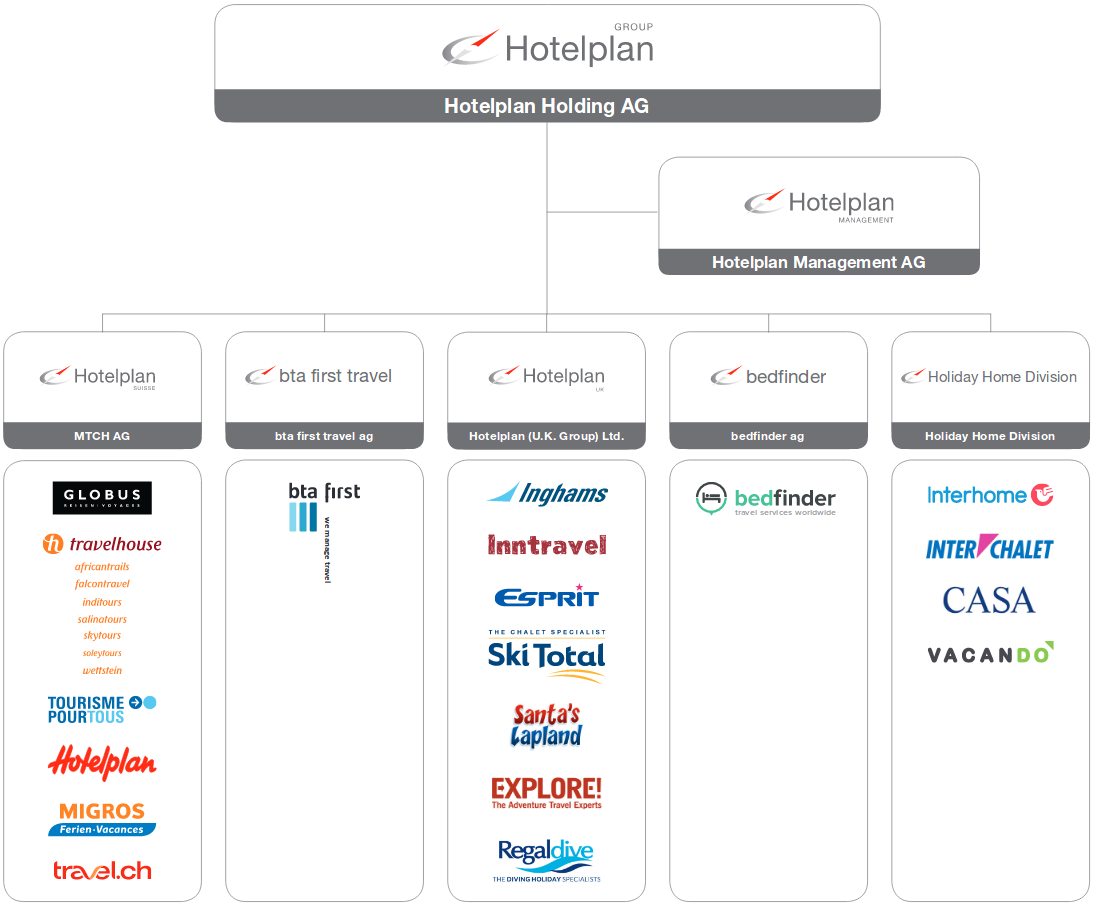
\includegraphics[width=0.7\textwidth]{images/organisationsstruktur}
	\caption{Organisationsstruktur der Hotelplan Group}
	\label{fig:einleitung:organisationsstruktur:1}
\end{figure}

In der \cref{fig:einleitung:organisationsstruktur:2} werden die Marken der verschiedenen \glspl{sbu} aufgeführt.
\begin{table}[h] 
	\caption{Markenaufstellung der Hotelplan Management AG}
	\centering
	\rowcolors{1}{tablebodycolor}{tablerowcolor}
	\label{fig:einleitung:organisationsstruktur:2}
	\begin{tabular}{ | c | c | c |} 
		\hline 		
		\rowcolor{tableheadcolor}
		\bfseries \gls{sbu} & \bfseries Marke & \bfseries Portal \\ \hline 
		Hotelplan Managment AG & Hotelplan Management & \href{http://www.hotelplan.com}{www.hotelplan.com} \\ \hline 
		MTCH AG & Globus Reisen & \href{http://www.globusreisen.ch}{www.globusreisen.ch} \\ \hline 
		MTCH AG & Travelhouse & \href{http://www.travelhouse.ch}{www.travelhouse.ch} \\ \hline 
		MTCH AG & Tourisme pour Tous & \href{http://www.tourismepourtous.ch/}{www.tourismepourtous.ch} \\ \hline 
		MTCH AG & Hotelplan & \href{http://www.hotelplan.ch}{www.hotelplan.ch} \\ \hline 
		MTCH AG & Migros Ferien & \href{http://www.migros-ferien.ch}{www.migros-ferien.ch} \\ \hline 
		MTCH AG & Travelwindow & \href{http://www.travel.ch}{www.travel.ch} \\ \hline 
		bta first travel ag & bta first & \href{http://www.btafirst.com}{www.btafirst.com} \\ \hline 
		Hotelplan UK & Inghams & \href{http://www.inghams.co.uk}{www.inghams.co.uk} \\ \hline 
		Hotelplan UK & Inntravel & \href{http://www.inntravel.co.uk}{www.inntravel.co.uk} \\ \hline 
		Hotelplan UK & Esprit & \href{http://www.esprit-holidays.co.uk}{www.esprit-holidays.co.uk} \\ \hline 
		Hotelplan UK & Ski Total & \href{http://www.skitotal.com}{www.skitotal.com} \\ \hline 
		Hotelplan UK & Santa's Lapland & \href{http://www.santaslapland.com}{www.santaslapland.com} \\ \hline 
		Hotelplan UK & Explore & \href{http://www.explore.co.uk}{www.explore.co.uk} \\ \hline 
		Hotelplan UK & Regaldive & \href{http://www.regal-diving.co.uk}{www.regal-diving.co.uk} \\ \hline 
		bedfinder ag & Bedfinder & \href{http://www.bedfinder.com}{www.bedfinder.com} \\ \hline 
		Holiday Home Division & Interhome & \href{http://www.interhome.ch}{www.interhome.ch} \\ \hline 
		Holiday Home Division & Interchalet & \href{http://www.interchalet.de}{www.interchalet.de} \\ \hline 
		Holiday Home Division & Casa & \href{http://casa.interchalet.de}{casa.interchalet.de} \\ \hline 
		Holiday Home Division & Vacando & \href{http://www.vacando.ch}{www.vacando.ch} \\ \hline 
	\end{tabular}
\end{table}

\section{Ziel der Arbeit}
\label{sec:einleitung:ziel}
Das Ziel der Arbeit ist es, Interhome eine Plattform zur Verfügung zu stellen, damit neue Informationen aus den Buchungsdaten extrahiert werden können (Knowledge Discovery). Dafür wird entweder ein bestehendes Programm verwendet oder eine eigene Lösung entwickelt. Es soll möglich sein, zum Beispiel eine folgende Frage zu beantworten: „Was für Objekte werden im Winter am meisten in Zermatt gebucht?“. Eine mögliche Antwort wäre: „Objekte welche unter CHF500 kosten und maximal 200 Meter von einem Skilift entfernt sind“.
Dies sollte Interhome ermöglichen, ihre Marketing Strategie zu verbessern und gezielter Objekte einzukaufen.

Um solche Fragen zu beantworten werden die Buchungsdaten von Interhome (Objekt, Zeitraum, Passagiere, etc.) verwendet und mit weiteren Daten (Geolocation, Wetterinformation) angereicht. 
Auf dem Endprodukt soll ein Mitarbeiter von Interhome in der Lage sein, ein Abfrage zu generieren, welche aus einem oder mehreren Attribute besteht. Die Applikation analysiert daraufhin die Daten mit Techniken des Data Mining, um eine Liste von Attributen zurück zu liefern, welche für die in der Abfrage aufgeführten Attributen am meisten Buchungen generieren. Die Elemente in der Antwort sollten gewichtet sein um das Resultat besser zu interpretieren.

Um dies besser zu veranschaulichen sollte hier ein Beispiel gemacht werden. Dazu ist in der \cref{fig:einletung:ziel:1} eine Datenmenge aufgeführt. Die ersten 9 Spalten sind Rohdaten und das Wetter (letzte Spalte) muss zusätzlich angereichert werden.

\begin{table}[h] 
	\caption{Beispielhafte angereicherte Buchungsdaten}
	\centering
	\rowcolors{1}{tablebodycolor}{tablerowcolor}
	\label{fig:einletung:ziel:1}
	\begin{tabular}{ | c | c | c | c | c | c | c | c | c | c |} 
		\hline 
		\rowcolor{tableheadcolor}
		\multicolumn{8}{|c|}{\bfseries Objektdaten} & \multicolumn{2}{c|}{\bfseries Kundendaten} \\ \hline
		
		\rowcolor{tableheadcolor}
		\bfseries \rotatebox{90}{ID} & \bfseries \rotatebox{90}{Ortschaft} & \bfseries \rotatebox{90}{Preis (CHF)} & \bfseries \rotatebox{90}{Tiere erlaubt} & \bfseries \rotatebox{90}{Grill vorhanden} & \bfseries \rotatebox{90}{Balkon vorhanden} & \bfseries \rotatebox{90}{Distanz zum Meer (m)} & \bfseries \rotatebox{90}{Distanz zum Skilift (m)} &  
		
		\bfseries \rotatebox{90}{Ortschaft} & \bfseries \rotatebox{90}{Wetter} \\ \hline 
		
		1 & Zermatt & 230 & \checkmark &  &  &  & 150 & Bern & Sonne \\ \hline 
		2 & Cannes & 450 & & \checkmark & \checkmark & 700 & &  Grindelwald & Schnee \\ \hline 
		3 & Zermatt & 2301 & \checkmark & \checkmark &  & 350 &  &  Mallorca & Regen \\ \hline 
		4 & Zermatt & 879 & \checkmark & & \checkmark &  & 350  & Nizza & Regen \\ \hline 
		5 & Zermatt & 149 & \checkmark &  & \checkmark &  & 500 & Zürich & \\
		6 & Cannes & 873 &  & \checkmark &  & 80 &  &  Mallorca & Regen \\ \hline 
		7 & Zermatt & 620 & \checkmark & \checkmark &  &  &  &  Zürich & Regen \\ \hline 
	\end{tabular}
\end{table}

Als Beispiel möchte das Marketing wissen, was gebucht wird wenn es regnet. Die Anfrage  lautet "`Wetter = Regen"'. Dies passt auf die Elemente mit den IDs 3, 4, 6 und 7 zu. Das Resultat der Datenanalyse \cref{fig:einletung:ziel:1} ist in diesem Fall "`Ortschaft = Zermatt, Tiere erlaubt = \checkmark, in 3/4 Buchungen"'. Oder in Worten: "`In 75\% der selektieren Buchungen wurden Objekte in Zermatt gebucht, in welchen Haustiere erlaubt sind."'. 

Die Daten können schlussendlich weiterverwendet werden, um gezielter Werbung an die Kunden zu bringen. Im obigen Beispiel könnte man durch die IP-Adresse des Users auf der Webseite von Interhome den ungefähren Ort herausfinden wo dieser wohnt. Durch weitere bestehende Services kann zusätzlich das momentane Wetter des Benutzers ermittelt werden. Ist es dort zur Zeit am regnen, kann dem Kunden Objekte in Zermatt angezeigt werden, in welchen Haustiere erlaubt sind.


\section{Abgrenzung}
\label{sec:einleitung:abgrenzung}
Dieses Kapitel beschreibt sämtliche Projektabgrenzungen, welche für dieses Projekt definiert
wurden.

\subsection{Zeitliche Abgrenzung}
Für diese Arbeiten geltet die zeitliche Vorgabe der \gls{zhaw} von 6 Monaten mit einem Arbeitsaufwand von 360 Stunden.
Der Start der Arbeit beginnt mit der Abnahme der Aufgabenstellung, welche am 04.11.2016 stattfand.
Demnach endet die Arbeit am 04.05.2017.

\subsection{Sachliche Abgrenzung}
Ziel der Arbeit ist es, eine Plattform zu schaffen auf welcher die Buchungsdaten von Interhome exploriert werden können. Dazu müssen die Daten aus dem Irent extrahiert und mit Techniken des Data Mining analysiert werden. Schlussendlich wird das Resultat bewertet, sodass entschieden werden kann ob es sich für einen produktiven Einsatz eignet.

Nicht beinhaltet in der Arbeit ist die Verbesserung der Marketing Strategie. Dies sollte durch das Projekt ermöglicht werden, ist jedoch nicht Teil davon. Zusätzlich könnte die Plattform nützlich sein, um personalisierte Werbung auf der Webseite von Interhome zu schalten. Dies ist jedoch auch nicht im Umfang der Arbeit enthalten.

\subsection{Projektbeteiligte}
\begin{table}[H] 
	\caption{Projektbeteiligte}
	\centering
	\rowcolors{1}{tablebodycolor}{tablerowcolor}
	
	\begin{tabular}{ | c | c | c | c |} 
		\hline 
		\rowcolor{tableheadcolor}
		\bfseries Beschreibung & 
		\bfseries Firma/Institution & 
		\bfseries Personen \\ \hline 
		Auftraggeber & Hotelplan Management AG & Christian Kiser \\ \hline 
		Projektleitung & Hotelplan Management AG & Simon Lang\\ \hline 
		Projektbetreuerin &  \gls{zhaw} & Dr. Ruxandra Domenig \\ \hline 
		Experte & \gls{zhaw} & Christioph Burkhardt \\ \hline 
	\end{tabular} 
\end{table}

\section{Vorgehen}
\label{sec:einletung:vorgehen}
Nachfolged wird das Vorgehen für die Analyse der Daten und die Umsetzung des Prototypen beschrieben.

Zuerst wird in der Recherche (siehe \cref{sec:recherche} \nameref{sec:recherche}) die Daten beschafft, welche im Rahmen dieser Arbeit zu untersuchen sind. Für das Data Mining werden verschiedene Techniken aufgeführt, welche sich für die Analyse eignen könnten. Zusätzlich werden noch existierende wissenschaftliche Arbeiten gesucht welche sich mit derselben Thematik auseinandersetzen. Zum Abschluss werden noch Programme evaluiert, welche für das Data Mining eingesetzt werden können.

Das zweite Kapitel widmet sich der Anforderungsanalyse (siehe \cref{sec:anforderungsanalyse} \nameref{sec:anforderungsanalyse}). Darin werden die Anforderungen an die Data Mining Techniken beschrieben, welche im Kapitel Recherche erläutert wurden. Zusätzlich werden Die Buchungsdaten analysiert und zuletzt die Voraussetzungen definiert, welche die Plattform für das Knowledge Discovery zu erfüllen hat.

Nachdem die Anforderungen festgelegt wurden wird ein Konzept (siehe \cref{sec:konzept} \nameref{sec:konzept}) erstellt. Dieses legt fest, welche Data Mining Techniken in der Arbeit verwendet werden. Zusätzlich werden folgende Punkte im Bezug an die Platform für das Knowledge Discovery definiert:
\begin{itemize}
	\item Wird ein bestehendes Programm verwendet oder eine eigene Implementation.
	\item Design und Funktionalität der Plattform.
	\item Testcases der Plattform.
\end{itemize}

Anschliessend startet das Proof of Concept (siehe \cref{sec:proofofconcept} \nameref{sec:proofofconcept}). Darin müssen zuerst die Daten für die Analyse vorbereitet werden. Danach wird die Plattform aufgesetzt oder implementiert.

Zum Abschluss werden die Testcases aus dem Konzept ausgewertet und ein Fazit gezogen.

\section{Grobplanung}
In der \cref{fig:einleitung:projektablaufplan} \nameref{fig:einleitung:projektablaufplan} ist der Projektablaufplan dargestellt.
\begin{sidewaysfigure}[h]
	\centering
	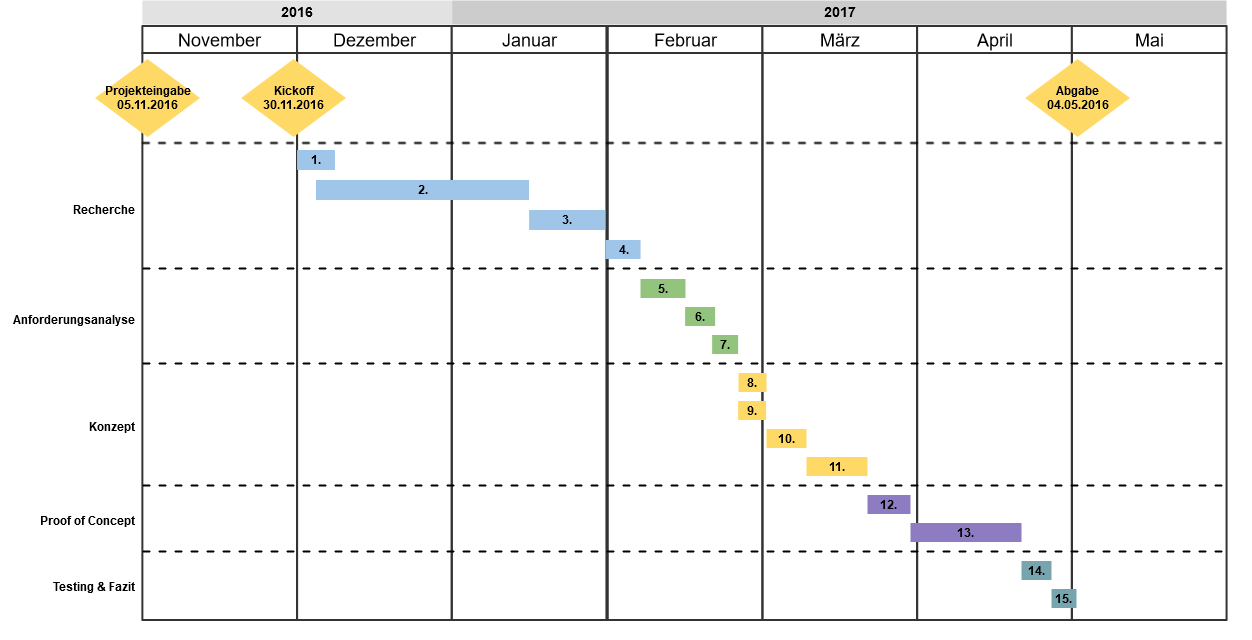
\includegraphics[width=1\textwidth]{images/projektablaufplan}
	\caption{Projektablaufplan}
	\label{fig:einleitung:projektablaufplan}
\end{sidewaysfigure}
\\\\
{\parindent0pt % disables indentation for all the text between { and }
Nachfolgend die Beschreibung der einzelnen Arbeitsschritte des Projektplanes.\\

Recherche:\\
1. Beschaffung der Buchungsdaten für die Auswertung.\\
2. Evaluation von verschiedenen Techniken des Data Mining, welche für die Auswertung der Daten verwendet werden können.\\
3. Vorhandene wissenschaftliche Arbeiten suchen, welche sich mit einer ähnlichen Problemstellung auseinandersetzen.\\
4. Evaluation von verschiedenen Programmen für die Auswertung und Darstellung der Daten.\\

Anforderungsanalyse:\\
5. Beschreibung der Vorgehensweisen, welche in wissenschaftlichen Arbeiten gefunden wurden und sich für die Problemstellung eignen. \\
6. Analyse der Buchungsdaten für die Auswertung.\\
7. Anforderungen an das Programm für die Auswertung und Darstellung der Daten.\\

Konzept:\\
8. Definition einer Vorgehensweise für die Datenanalyse.\\
9. Festlegen ob ein Programm für die Auswertung und Darstellung der Daten verwendet wird oder eine eigene Implementation.\\
10. Design und Funktionalität des Programmes definieren.\\
11. Definition der Testcases an das Programm.\\

Proof of Concept:\\
12. Vorbereitung der Daten für die Auswertung.\\
13. Erstellung oder Verwendung eines Programmes für die Analyse und Darstellung der Daten.\\

Testing \& Fazit\\
14. Auswertung der Testcases.\\
15. Einschätzung ob das Programm live für Interhome eingesetzt werden kann.
}

\section{Begriffsdefinition}
\label{sec:einletung:begriffsdefinition}
In der Arbeit werden durchgehend einige Begriffe verwendet welche hier erläutert werden. Für ein besseres Verständnis wird zuerst noch der Aufbau eines Objektes von Interhome aufgezeigt.

\cref{fig:einletung:begriffsdefinition:2} zeigt ein Objekt von Interhome wie es auf der Webseite \href{https://www.interhome.ch/de}{www.interhome.ch} gezeigt wird. Rot hinterlegt ist die Identifikation des Appartments. Diese wird ID oder im Interhome Jargon auch NREF genannt. Die grundlegenden Infos wie der Name des Objektes, wo es liegt, wie viele Sterne es hat, etc. ist im grünen Bereich ersichtlich. Die Preise und allfällige Aktionen sind im blauen Kasten und weitere Charakteristiken des Objektes zuunterst im gelben Bereich aufgeführt. Die Bilder werden in Analyse der Daten nicht verwendet weshalb sie nicht näher erläutert werden.
\begin{figure}[h]
	\centering
	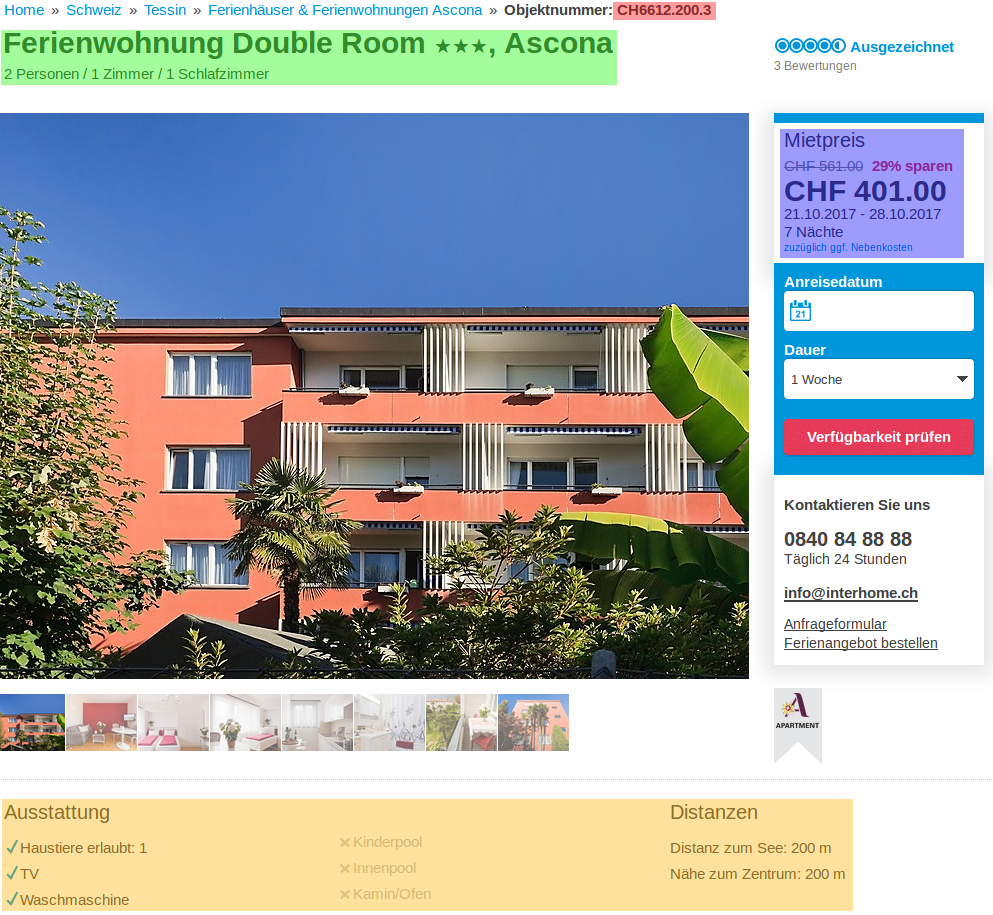
\includegraphics[width=1\textwidth]{images/interhome-object}
	\caption{Erklärung eines Interhome Objektes.}
	\label{fig:einletung:begriffsdefinition:2}
\end{figure}

Die zu erklärenden Begriffe sind in der \cref{fig:einletung:begriffsdefinition:1} aufgeführt. Diese werden im Text sowie in Formeln verwendet, weshalb zusätzlich zur Erklärung noch eine Variable definiert wurde.

\begin{table}[H] 
	\caption{Begriffsdefinition}
	\centering
	\rowcolors{1}{tablebodycolor}{tablerowcolor}
	\label{fig:einletung:begriffsdefinition:1}
	\begin{tabular}{ | c | C{2.5cm} | p{10cm} |} 
		\hline 
		\rowcolor{tableheadcolor}
		\bfseries Var & 
		\bfseries Begriff & 
		\bfseries Beschreibung \\ \hline 
		$A$ & Attribut & Ein Feld mit einem Wert. 1-n Attribute bilden eine Instanz. Beispiele:\
			\begin{itemize}
			\item ID: 5
			\item Distanz bis zum Meer: Nahe / Fern
			\item Sauna vorhanden: \checkmark
			\end{itemize} \\ \hline 
		$I$ & Instanz & Zusammenfassung von Attributen. 0-n Instanzen bilden eine Datenmenge. Nachfolgend wird ein Beispiel gezeigt, wie ein Objekt von Interhome vereinfacht aufgebaut sein könnte. Alle Attribute zusammen bilden eine Instanz.\
			\begin{itemize}
			\item ID: CH1000.400.1
			\item Preis (CHF): 500
			\item Sauna vorhanden: \checkmark
			\end{itemize} \\ \hline 
		$D$ & Datenmenge & In dieser Arbeit ist damit die Gesamtheit aller Buchungen von Interhome zu verstehen. Im folgenden Beispiel sind die Instanzen als Tupel dargestellt in der Form (ID, Preis, Anzahl Zimmer). Alle zusammen bilden die Datenmenge.\
			\begin{itemize}
			\item (CH1000.400.1, CHF500, 5)
			\item (CH1000.400.2, CHF340, 2)
			\end{itemize}\\ \hline 
		%$K$ & Konzept & Hypothesen über die Daten. \ z.B. Wenn jemand Bier kauft, dann meistens auch Windeln. \\ \hline 
		$A^c$ & Kategorische Attribute & Attribute welche eine endliche Anzahl von Ausprägungen annehmen können. In dieser Arbeit haben kategorische Attribute keine Reihenfolge. Z.B.: \
			\begin{itemize}
			\item Saune vorhanden: \checkmark, \ding{55}
			\item Distanz bis zum Meer: Nahe, Fern
			\end{itemize} \\ \hline
		$A^n$ & Numerische Attribute & Attribute welche eine reele Zahl $\mathbb{R}$ annehmen können.\\ \hline
		& i-Attributmenge & Eine Menge mit i Attributwerten. Z.B.:
			\begin{itemize}
			\item 1-Attributmenge: { (ID, 5) }
			\item 2-Attributmenge: { (ID, 5), (Preis, CHF500)}
			\end{itemize}\\ \hline 
	\end{tabular} 
\end{table}
\chapter{Recherche}
\label{sec:recherche}
\todo{desc}


\section{Datenbeschaffung}
\label{sec:recherche:datenbeschaffung}
Als erstes wurden die Daten für die Auswertung beschafft. Diese mussten aus dem \gls{irent} extrahiert werden. Dies musste von einer anderen Abteilung erledigt werden da nur Sie Zugriff auf die Export-Funktion des System haben. Da die Buchungen Kundendaten enthalten, können Sie nicht veröffentlicht werden.

Die Daten liegen im Windows Excel Format vor. Es sind total 133'001 Datensätze mit jeweils 153 Felder. Die Zellen A-U sind Informationen im Bezug auf die Buchungen, alle anderen (V-EW) beziehen sich auf das Objekt selber. Die Felbeschreibungen sind im \cref{app:feldbeschreibungen} \nameref{app:feldbeschreibungen} aufgeführt.

\section{Prozess des Data Mining}
\label{sec:recherche:dataminingtechniken}
Unter Data Mining versteht man die Anwendung von statistischen Methoden auf grossen Datenmengen mit dem Ziel, neue Erkenntnisse zu gewinnen.

Data Mining sieht folgende Schritte vor:
\begin{enumerate}
	\item Datenbeschaffung
	\item Daten vorbereiten
	\item Methoden zur Gewinnung von Informationen anwenden
	\item Überprüfung der Resultate
\end{enumerate}

Schritt 1 ist die Beschaffung der Daten, welche analysiert werden sollen (siehe \cref{sec:recherche:datenbeschaffung} \nameref{sec:recherche:datenbeschaffung}). 

Die Vorbereitung der Daten Bereinigt, Transformiert und Reduziert Informationen und wird im \cref{sec:recherche:dataminingtechniken:datenvorbereiten} \nameref{sec:recherche:dataminingtechniken:datenvorbereiten} beschrieben.

Der dritte Punkt ist das eigentliche Datengewinnung. Dabei werden Methoden des Data Mining auf die Daten angewendet. Mögliche Vorgehensweisen werden im \cref{sec:recherche:dataminingtechniken:disziplinen} \nameref{sec:recherche:dataminingtechniken:disziplinen} beschrieben.

Beim letzten Schritt werden die Resultate überprüft. Ist das Resultat nicht zufriedenstellend, so werden Punkt 2-4 wiederholt.

\subsection{Daten vorbereiten}
\label{sec:recherche:dataminingtechniken:datenvorbereiten}

Danach müssen die Daten vorbereitet werden. Dies umfasst die Bereinigung, Transformation sowie Reduktion von Informationen\footcite{feature_selection_2017-01-04}. Bei ersteren werden Messfehler behoben, fehlende Felder ergänzt oder Duplikate entfernt. Die Transformation wandelt Werte um damit sie für die Berechnung besser geeignet sind. Zum Beispiel können Wertebereiche in Intervalle aufgeteilt werden. Bei letzteren werden Instanzen der Datengrundlage entfernt, wodurch die Berechnungszeit verkürzt wird, oder Attribute von allen Instanzen entfernt, da deren Entropie zu gering ist. Weiteres hierzu im \cref{sec:proofofconcept:datenvorbereitung} \nameref{sec:proofofconcept:datenveorbereitung}. 


\subsection{Disziplinen im Data-Mining}
\label{sec:recherche:dataminingtechniken:disziplinen}
Die folgenden Methoden geben eine Übersicht über die gängigsten Techniken wider. Später wird im \cref{sec:konzept:vorgehensweise} \nameref{sec:konzept:vorgehensweise} eine Methode ausgewählt und genauer beschrieben. 

\subsubsection{Association rule learning}
Bei Association rule learning (Assoziationsanalyse) handelt es sich um \gls{supervisedlearning} wobei Korrelationen zwischen Attributen aufgedeckt werden. Bei einer Warenkorbanalyse kann dadurch erkannt werden, welche Produkte die Kunden oft zusammen eingekaufen.

Der Prozess in der Assoziationsanalyse besteht aus zwei Schritten. Zuerst werden häufig auftretende Attributkombinationen gesucht, aus welchen anschliessend Regeln generiert werden\footcite{association_rule_learning_2017-01-05}.

Im Falle einer Warenkorbanalyse könnte eine Regeln die Form "Samstags wenn ein Kunde Käse und Brot kauft, dann kauft er auch Liquor". Oder im Falle von Interhome "Wenn ein Kunde eine Ferienwohnung mit Pool am Meer bucht, dann besitzt das Objekt auch eine Klimaanlage".

\subsubsection{Classification}
\label{sec:recherche:dataminingtechniken:disziplinen:classification}
Das Ziel der Classification (Klassifikation) ist es, eine Instanz einer Klasse zuzuweisen. Dies könnte die Kreditwürdigkeit eines Kunden sein. Die Klassen sind dabei vordefiniert, wodurch es um ein \gls{supervisedlearning} handelt.

Es gibt verschiedene Techniken für die Zuweisung einer Instanz zu einer Klasse. Es können Entscheidungsregeln, Bayes-Klassifikatoren, neurale Netze und weitere verwendet werden\todo{cite}. Entscheidungsregeln können als Bäume dargestellt werden und sind visuell einfach verständlich.

\begin{figure}[H]
	\centering
	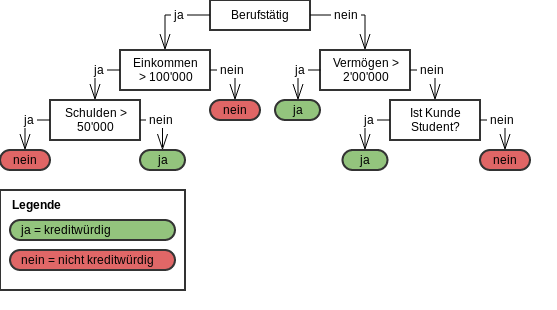
\includegraphics[width=0.8\textwidth]{images/decision_tree.png}
	\caption{Entscheidungsbaum für die Kreditwürdigkeit eines Kunden.}
	\label{fig:recherche:dataminingtechniken:disziplinen:classification}
\end{figure}

\cref{fig:recherche:dataminingtechniken:disziplinen:classification} zeigt einen Entscheidungsbaum, welcher von oben nach unten durchlaufen wird. Die Quadrate sind Entscheidungen, und bei den Ovalen handelt es sich um Zuweisungen zu der Klasse "`kreditwürdig"'.

% Evt. noch was schreiben über Training- und Testdaten

\subsubsection{Regression}
Bei der Regresseion wird von einer abhängiger Variable Y auf eine unabhängige Grösse X zurückgeschlossen\todo{korrekt?}. Man spricht dann von einer Regression von Y auf X. Dabei werden bestehende Daten auf einem Koordinatensystem aufgetragen und eine Funktion definiert oder gesucht, welche die Messungen möglichst genau annähert. Für eine gegebene abhängige Variable kann somit die unabhängige Grösse errechnet werden\todo{cite}. 

\cref{fig:recherche:dataminingtechniken:disziplinen:regression} zeigt das Resultat einer linearen Regression.

\begin{figure}[H]
	\RawFloats
	\centering
	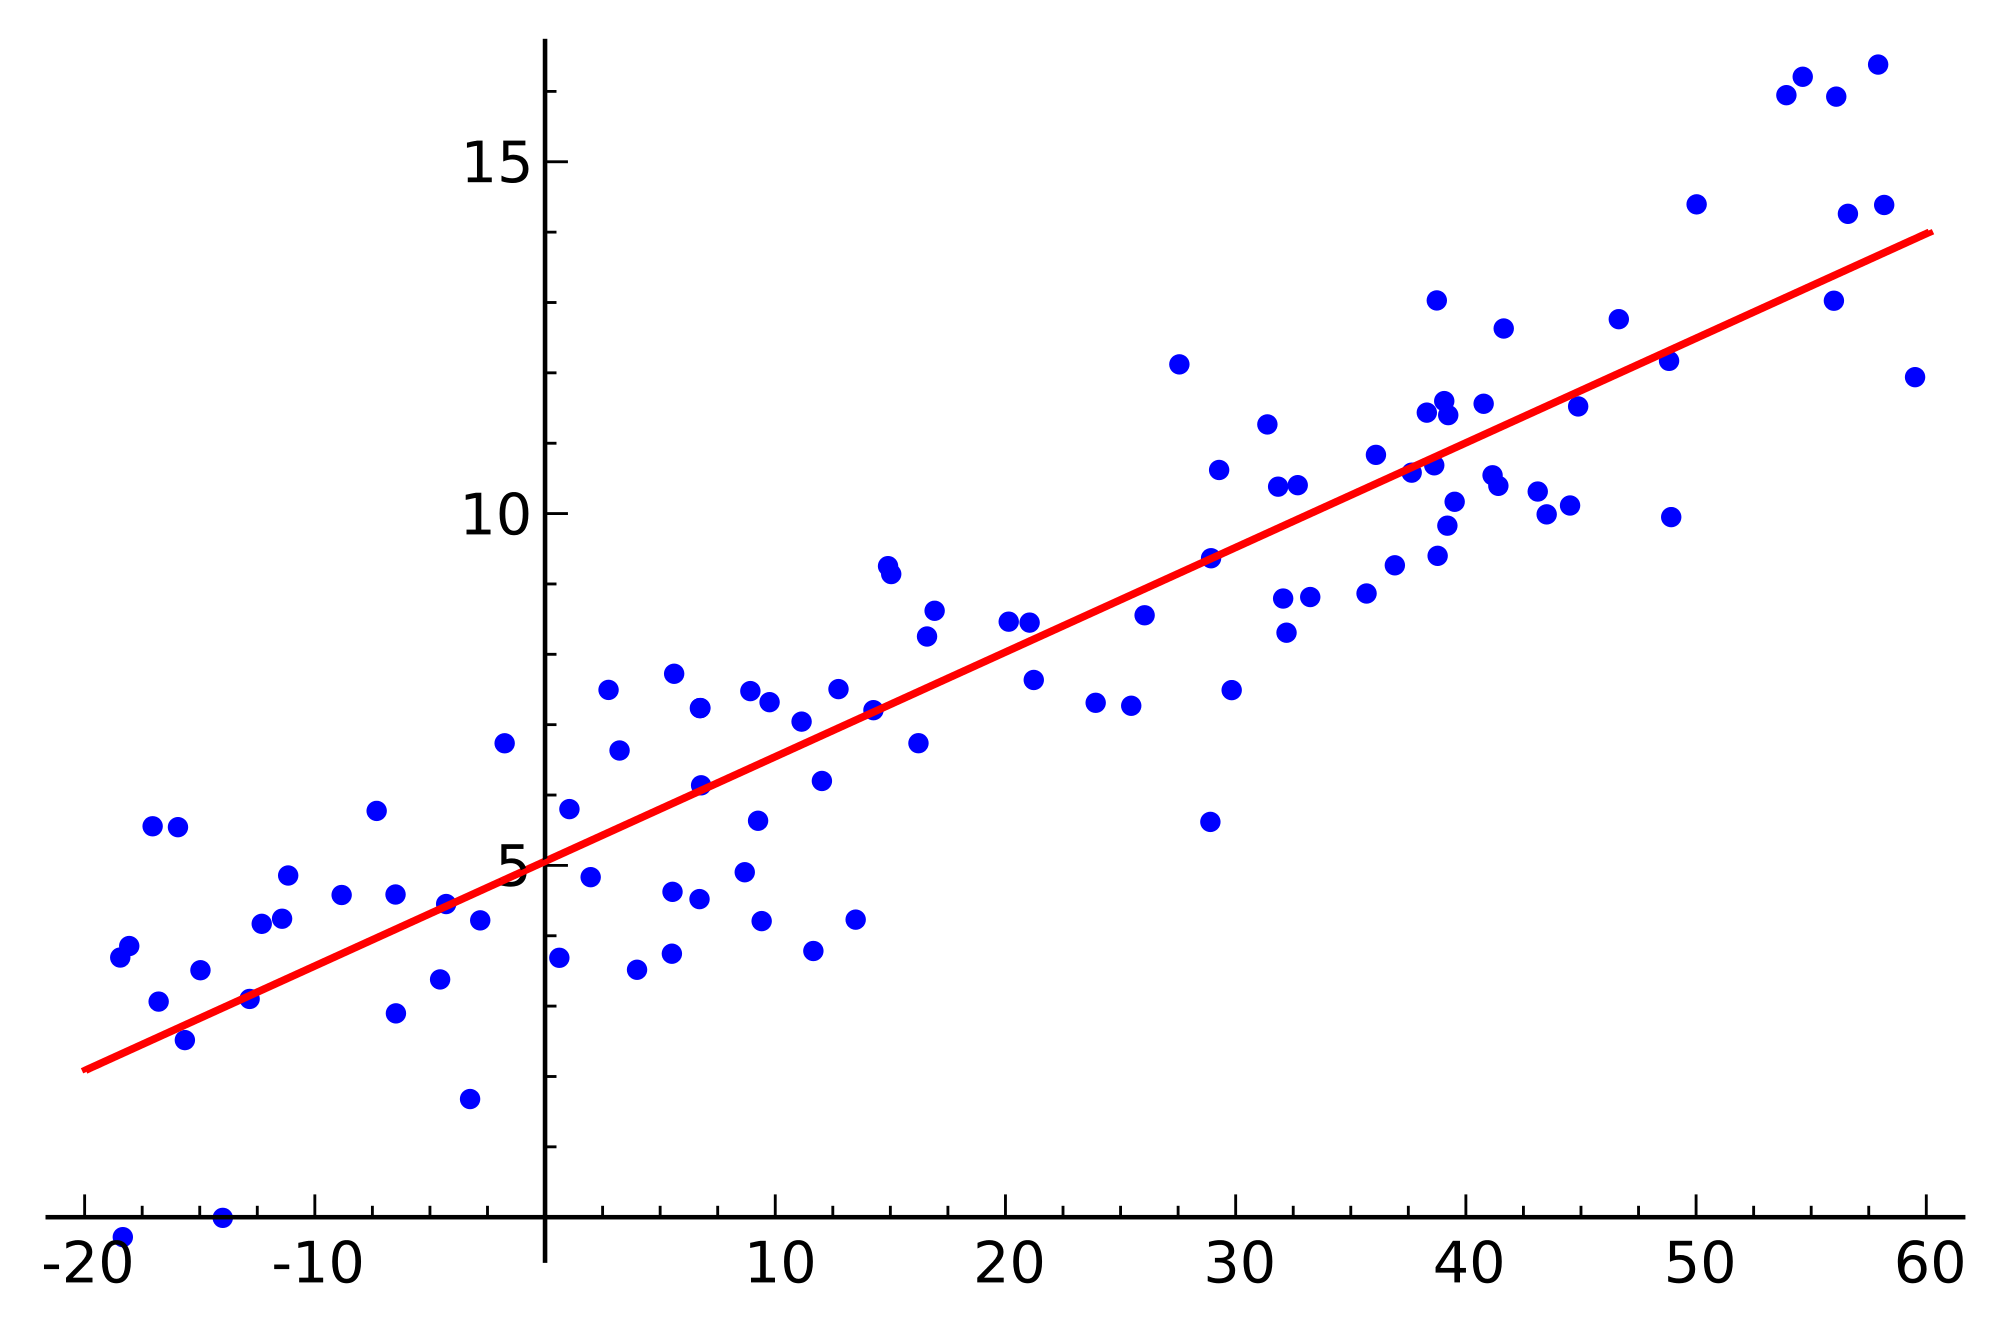
\includegraphics[width=0.8\textwidth]{images/Linear_regression.png}
	\caption{Gerade einer linearen Regression durch eine Punktwolke}
	\source{\cite{Linear_regression_2017-01-08}}
	\label{fig:recherche:dataminingtechniken:disziplinen:regression}
\end{figure}

\subsubsection{Cluster analysis}
\label{sec:recherche:dataminingtechniken:disziplinen:clusteranalysis}
Die Cluster analysis (Clusteranalyse) weist, ähnlich zur \nameref{sec:recherche:dataminingtechniken:disziplinen:classification}, den Instanzen eine Klasse zu. Jedoch sind diese zu beginn nicht bekannt, wodurch es sich um ein \gls{unsupervisedlearning} handelt.

In \cref{fig:recherche:dataminingtechniken:disziplinen:clusteranalysis} sind Punkte in einem Koordinatensystem eingetragen. Diese werden bei der Clusteranalyse in mehrere Gruppen unterteilt, welche die Klassen abbilden. Im Gegensatz zur \nameref{sec:recherche:dataminingtechniken:disziplinen:classification} haben diese jedoch keine weitere Bedeutung, sondern geben nur an dass sie ähnlich zu allen anderen Instanzen im selben Cluster sind. Je nach Verfahren ist es unterschiedlich, wie viele Klassen gebildet werden oder ob die Anzahl vorgegeben ist\todo{cite}.
\begin{figure}[H]
	\RawFloats
	\centering
	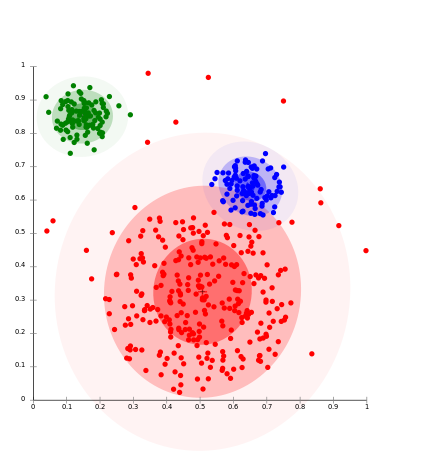
\includegraphics[width=0.8\textwidth]{images/clusteranalysis.png}
	\caption{Koordinatensystem für eine Cluster analysis}
	\source{\cite{Cluster_analysis_2017-01-08}}
	\label{fig:recherche:dataminingtechniken:disziplinen:clusteranalysis}
\end{figure}

Eingesetzt wird die Clusteranalyse zum Beispiel für die Erkennung von Kundengruppen oder zur  Zusammenfassung und Vergleich gleichartiger Produkten\footcite{einsatzgebiet_clusteranalyse}.


\subsubsection{Collaborative Filtering}
Beim Collaborative Filtering (kollaboratives Filtern) wird zu einer Instanz ähnliche Objekte gesucht. Die Ähnlichkeit wird durch Bewertung von anderen Kunden errechnet. 

\begin{table}[H] 
	\caption{Begriffsdefinition}
	\centering
	\rowcolors{1}{tablebodycolor}{tablerowcolor}
	\label{fig:recherche:dataminingtechniken:disziplinen:collaborativefiltering}
	
	\begin{tabular}{ | l | c | c | c | c |} 
		\hline 
		\rowcolor{tableheadcolor}
		\bfseries & 
		\bfseries Maria & 
		\bfseries Sandro & 
		\bfseries Urs & 
		\bfseries Heidi \\ \hline 
		\textbf{Pulp Fiction} & - & - &  & + \\ \hline 
		\textbf{The Matrix} & + & + & + & - \\ \hline 
		\textbf{American Hustle} & - & + &  & + \\ \hline 
		\textbf{12 Monkeys} & + & + & - & \cellcolor{yellow!75}? \\ \hline 
	\end{tabular} 
\end{table}

Die Zeilen in der \cref{fig:recherche:dataminingtechniken:disziplinen:collaborativefiltering} sind Instanzen und die Spalten zeigen Bewertungen der Kunden. Minus steht für eine negative und Plus für eine positive Bewertung. Es ist auch möglich das ein Benutzer eine Instanz nicht bewertet. Mittels kollaborativen Filtern kann nun abgeschätzt werden, ob ein Benutzer eine Instanz positiv oder negativ Bewertet\todo{cite}.

\section{Wissenschaftliche Arbeiten}
\todo{}

\section{Programmevaluation}
Auf dem Markt gibt es diverse Data Mining Programme von welchen hier einige vorgestellt werden.

Zwingend notwendig ist es, dass das Programm gratis ist, sowie unter den Betriebsystemen Windows sowie Linux lauffähig ist. 

%http://thenewstack.io/six-of-the-best-open-source-data-mining-tools/

\subsection{RapidMiner Studio}
RapidMiner, früher YALE (Yet Another Learning Environment) wurde von der Technischen Universität Dortmund entwickelt und bietet eine kostenlose Version an, welche auf 10'000 Datensätze und einen logischen Prozessor beschränkt ist. Es gibt jedoch für Studenten eine Version mit welcher beliebig Grosse Daten bearbeitet werden können. Die Applikation ist in Java geschrieben und somit auf allen gängigen Betriebssystemen lauffähig\footcite{RapidMiner_Studio_2017-01-14}.

RapidMiner Studio bietet für eine grosse Anzahl an Algorithmen fertige Bausteine an, welche verwendet werden können. Alle unter \cref{sec:recherche:dataminingtechniken:disziplinen} \nameref{sec:recherche:dataminingtechniken:disziplinen} aufgeführten Methoden sind in der Applikation als Operatoren implementiert und können durch einige klicks verwendet werden. Eine Auflistung aller Operatoren ist in der RapidMiner Dokumentation aufgeführt: \url{http://docs.rapidminer.com/studio/operators/}

\subsection{WEKA}
\gls{weka} ist ein in Java entwickeltes Programm der University of Waikato, New Zealand. Veröffentlicht wurde die Software unter der \gls{acr:gnugpl} und ist somit frei verfüg- und modifizierbar\footcite{Weka_2017-01-14}.

WEKA beherscht Classification, Clustering, Regression und Associating Algorithmen und deckt somit alle  im \cref{sec:recherche:dataminingtechniken:disziplinen} aufgeführten Disziplinen ab\footcite{Weka_Doc_2017-01-14}\footcite{Weka_Regression_2017-01-14}.



% Eigener Beitrag: Beschreibung, Begründung, Aufzeigung, Methode, Fazit

\chapter{Anforderungsanalyse}
\label{sec:anforderungsanalyse}

\section{Algorithmen}
\label{sec:anforderungsanalyse:algorithmen}
Dieser Abschnitt erläutert die Anforderungen welche an die Algorithmen gestellt werden.

\subsection{Komplexität}
\label{sec:anforderungsanalyse:algorithmen:komplexitaet}
Die Algorithmen sollten maximal ein super-lineares Wachstum ($\mathcal{O}(n\,log\,n)$) aufweisen. Diese Einschränkung ermöglicht die Erkundung der Daten im Programm ohne lange Wartezeiten zu generieren\todo{apriori O(n log n)?}.

\subsection{Mixed data types}
\label{sec:anforderungsanalyse:algorithmen:mixed-data-types}
Da die Buchungen von Interhome numerische (z.B. Anzahl Personen, Geolocations) und kategorische Daten (z.B. Aircondition vorhanden?, Objekttyp) beinhalten, müssen die Algorithmen in der Lage sein mit beiden Datentypen umgehen zu können.

\subsection{Resultat des Algorithmus}
\label{sec:anforderungsanalyse:algorithmen:resultat}
Ein Algorithmus muss Attribute als Resultat zurückliefern, damit die Fragenstellungen aus Kapitel 1\todo{cref} beantwortet werden können. Alternativ können auch Gruppen von Buchungen ausgegeben werden, in welchen anschliessend die Häufigkeiten der Attribute nachgezählt werden müssen. Auf jeden Fall müssen schlussendlich Attribute und deren Häufigkeiten eruiert werden können.

Zusätzlich muss ein Algorithmus selbständig Muster erkennen können, da bislang noch keine Informationen zu den Daten vorhanden sind. Es wird demnach ein \gls{unsupervisedlearning} durchgeführt.

\section{Programm}
\label{sec:anforderungsanalyse:programm}
Im \cref{sec:recherche:programmevaluation} wurden zwei Programme für das Data Mining vorgestellt. Hier werden die Anforderungen aufgelistet, welche diese Programme zu erfüllen haben, damit sie im weiteren Verlauf dieser Arbeit verwendet werden können.

\subsection{Lizenzen}
\label{sec:anforderungsanalyse:programm:lizenzen}
Die Applikation sollte kostenlos einsetzbar sein. Sie benötigt demnach eine der folgenden Lizenzmodellen:
\begin{itemize}
\item OpenSource. Software kann verwendet und angepasst werden (siehe \url{https://opensource.org/licenses}).
\item Freeware. Software kann verwendet, jedoch nicht angepasst werden.
\item Studenten Lizenz. Software kann als Student kostenlos eingesetzt werden.
\end{itemize}

\subsection{Betriebsystem}
\label{sec:anforderungsanalyse:programm:betriebsystem}
Die Entwicklung wird privat auf einem Linux Rechner durchgeführt, und Zeitweise auch bei der Arbeit auf Windows Computern welche von Hotelplan Management AG bereitgestellt werden.
Demnach ist es nötig, dass die Software unter Linux sowie auch Windows gestartet werden kann.

\subsection{Funktionsumfang}
\label{sec:anforderungsanalyse:programm:funktionsumfang}
Da der Datenbestand 133'001 Einträge umfasst, muss die Plattform und das Lizenzmodel diese Anzahl an Items unterstützen.

Zusätzlich muss das Programm die im \cref{sec:recherche:dataminingtechniken:disziplinen} \todo{fix cref} beschriebenen Techniken beherrschen.

\section{Funktionsumfang}
Das Programm muss für die Gewinnung neues Wissens aus der bisherigen Buchungen von Interhome gestaltet werden. Dazu sollen Algorithmen evaluiert werden welche folgende beispielhaften Fragestellungen beantworten können:
\begin{enumerate}
\item Welche Attribute werden im Winter wenn schneit in der Schweiz gebucht?
\item Welche Häuser im Tessin mit Sicht auf einen See werden am meisten gebucht?
\end{enumerate}

Als Antwort sollte der Algorithmus eine Liste von Attributen zurückliefern. Auf die obigen Beispiele könnte dies folgendes sein:
\begin{enumerate}
\item Objekte in Süditalien mit einem Pool.
\item Luxushäuser mit einem Grill und 3 Zimmern.
\end{enumerate}

Zusätzlich sollte nachvollziehbar sein, wieso der Algorithmus diese Attribute gewählt hat. Jede Eigenschaft sollte demnach mit einer Anzahl oder einer Prozentzahl versehen sein. Zum Beispiel:
\begin{enumerate}
\item Sütitalien (223 von 319) und Pool (150 von 319)
\item Luxushäuser (53\%), Grill (35\%) und 3 Zimmer (32\%)
\end{enumerate}
\chapter{Konzept}
\label{sec:konzept}

\section{Analyse der Buchungsdaten}
\todo{...}

\section{Einschränkung der Data Mining Disziplinen}
\label{sec:konzept:disziplinauswahl}
Ziel dieser Arbeit ist es, Attribute von Objekten zu eruieren, welche in einer Gruppe von Buchungen oft vorkommen\todo{cref zu Kapitel 1}. Nachfolgend wird anhand dieser Aufgabenstellungen entschieden, welche Disziplinen im Data Mining (siehe \cref{sec:recherche:dataminingtechniken:disziplinen} \nameref{sec:recherche:dataminingtechniken:disziplinen}) sich dazu eignen. Als Grundlage der Entscheidung gelten die Anforderungen welche an die Algorithmen gestellt wurden (siehe \cref{sec:anforderungsanalyse:algorithmen} \nameref{sec:anforderungsanalyse:algorithmen}).

\subsection{Association rule learning}
\label{sec:konzept:disziplinauswahl:association}
Mittels Association rule learning (siehe \cref{sec:recherche:dataminingtechniken:disziplinen:association} \nameref{sec:recherche:dataminingtechniken:disziplinen:association}) lassen sich aus allen selektierten Buchungen die Häufigkeiten von Attributkombinationen herausfinden. Dadurch kann die Fragestellung beantwortet werden.


\subsection{Classification}
\label{sec:konzept:disziplinauswahl:classification}
Bei der Classification handelt es sich um ein \gls{supervisedlearning} (siehe \cref{sec:recherche:dataminingtechniken:disziplinen:classification} \nameref{sec:recherche:dataminingtechniken:disziplinen:classification}). Deshalb sind vorab Klassen zu definieren welche den Objekten zugewiesen werden. Diese Informationen sind jedoch noch nicht vorhanden, weshalb in den Anforderungen (siehe \cref{sec:anforderungsanalyse:algorithmen:resultat} \nameref{sec:anforderungsanalyse:algorithmen:resultat}) ein \gls{unsupervisedlearning} Algorithmus vorausgesetzt wurde. Deshalb eignet sich die Classification für diese Aufgabenstellung nicht.

\subsection{Regression}
\label{sec:konzept:disziplinauswahl:regression}
Regression Algorithmen suchen eine Formel, damit man von einer abhängiger Variable auf unabhängige Grössen schliessen kann (siehe \cref{sec:recherche:dataminingtechniken:disziplinen:regression} \nameref{sec:recherche:dataminingtechniken:disziplinen:regression}). Damit kann man bei den Interhome Daten für neue Buchungen Attribute voraussagen. zum Beispiel wenn man die Kreditwürdigkeit von Kunden überprüfen möchte auf Basis von alten Buchungen.

Diese Algorithmen eignen sich jedoch nicht für diese Arbeit, da weder Attribute noch Gruppen von Buchungen zurückgeliefert werden (siehe \cref{sec:anforderungsanalyse:algorithmen:resultat} \nameref{sec:anforderungsanalyse:algorithmen:resultat}).

\subsection{Cluster analysis}
\label{sec:konzept:disziplinauswahl:clusteranalysis}
Das Resultat einer Cluster analysis sind Gruppen (Clusters) von Buchungen, die untereinander ähnlich, und zu allen anderen Gruppen möglichst unähnlich sind (siehe \cref{sec:recherche:dataminingtechniken:disziplinen:clusteranalysis} \nameref{sec:recherche:dataminingtechniken:disziplinen:clusteranalysis}). Da die Instanzen innerhalb des Clusters ähnlich zueinander sind, ist zu erwarten dass eine Häufigkeitszählung der Attribute innerhalb der Clusters aufzeigt, welche Eigenschaften besonders oft miteinander gebucht werden. Unter Berücksichtigung dieser Annahme eignen sich diese Algorithmen für die Beantwortung der Fragestellung.

\subsection{Collaborative Filtering}
\label{sec:konzept:disziplinauswahl:collaborativefiltering}
Collaborative Filtering werden für recommender systems eingesetzt um dem Benutzer Instanzen vorzuschlagen die er auch mögen könnte. Grundlage für diese Entscheidungen sind seine bisherigen Interaktionen mit dem System verglichen mit denen von anderen Benutzern. Dadurch könnte bei den Interhome Daten Objekte vorgeschlagen werden die der Kunde auch mögen könnte. Es werden jedoch keine Attribute oder Instanzgruppen gebildet, womit die Anforderung \cref{sec:anforderungsanalyse:algorithmen:resultat} nicht erfüllt sind.


\section{Algorithmenauswahl}
\label{sec:konzept:algorithmenauswahl}
Im \cref{sec:konzept:disziplinauswahl} wurden die Disziplinen auf Association rule learning und Cluster analysis eingeschränkt und im \cref{sec:recherche:algorithmen} die einzusetzenden Algorithmen beschrieben. Nachfolgend wird beschrieben wieso jene Abläufe ausgewählt wurden.

\subsection{Apriori}
Das Association rule learning besteht aus zwei Schritten. Zuerst werden mittels des Apriori Algorithmus häufige Attributkombinationen gesucht und anschliessend Regeln aufgestellt um Korrelationen zwischen gemeinsam auftretenden Eigenschaften aufzuzeigen.
Der zweite Schritt wird nicht benötigt, da die Regeln für die Aufgabenstellung dieser Arbeit nicht benötigt werden.

Es gibt Alternativen zum Apriori Algorithmus. Dies sind zum Beispiel der AprioriTid oder AprioriHybrid. Diese generieren die identischen Resultate und unterscheiden sich nur in der Laufzeit. Der AprioriTid kann zu beginn der Häufigkeitszählung bessere Leistung aufzeigen, ist jedoch langsamer gegen dessen Ende. Der AprioriHybrid verwendet zu Beginn der Apriori, und am Schluss den AprioriTid\footcite{association_rule_learning_2017-01-05}. 

Es ist noch unklar, welcher Algorithmus die besseren Laufzeiten aufweist. Zum Schluss oder nach der Arbeit kann in einer Vertiefung der AprioriTid oder der AprioriHybrid eingesetzt werden um die Leistungen der Algorithmen zu vergleichen. Im ersten Schritt wird der Apriori benutzt um zu analysieren ob die Resultate brauchbare Informationen liefern.

\subsection{Clustering}
\label{sec:konzept:algorithmenauswahl:clustering}
Es gibt diverse Algorithmen welche sich verschiedene Problemstellungen annehmen. Unterteilen lassen sich diese in vier Gruppen:
\begin{itemize}
	\item Partitioning
	\item Hierarchical
	\item Density-based
	\item Grid-mased
\end{itemize}
Nicht alle Algorithmen lassen sich eindeutig einer Gruppe zuweisen. Jedoch hilft diese Auflistung eine Übersicht über die Verfahren zu geben\footcite{data_mining_concepts_and_techniques}.

Für die Auswahl eines Algorithmus müssen die Charakteristiken der Daten bekannt sein, wie diese zum Beispiel verteilt (z.B. Kugel-, Kreis-, S-Förmig) oder wie viele Cluster sinnvoll sind. Diese sind bislang jedoch noch bekannt.
Partitioning- und Hierarchical-Vorgehensweisen benötigen zur Berechnung der Clustern deren Anzahl. Bei ersteren kann diese anhand der Elbow-Method berechnet werden\footcite{elbow_method}. Bei Hierarchischen Clustern müsste man dies jedoch für jeden Ast ermittelt. Da die Laufzeit von solchen Algorithmen bereits $\mathcal{O}(k^2)$ beträgt ist diese Vorgehensweise nicht praktikabel\footcite{complexity_hierarchical_clustering} (siehe \cref{sec:anforderungsanalyse:algorithmen:komplexitaet} \nameref{sec:anforderungsanalyse:algorithmen:komplexitaet}). Grid-based Methoden unterteilen den Datenraum in ein Netz wodurch die Clusters erzeugt werden. Unterstützt werden dabei nur numerische Daten weshalb sich diese Gruppe nicht eignet (weitere Forschung in dem Bereich ist jedoch im Gange\footcite{sting_categorical_data}).
Aus diesen Gründen werden in dieser Arbeit ein Vertreter aus der Partitioning (k-prototype) und der Density-based (DBSCAN) Gruppen umgesetzt.


\subsubsection{Distanzmessung}
\label{sec:konzept:algorithmenauswahl:clustering:distanzmessung}
Um die Resultate der Algorithmen zu vergleichen wird eine einheitliche Funktion $d$ zur Distanzmessung definiert.
Dazu eignet sich zum Beispiel die quadratische euklidische Distanz wie sie in der \cref{eq:recherche:clusteranalysis:1} aufgezeigt wird.

\begin{equation} \label{eq:recherche:clusteranalysis:1}
d(I_i, I_j) = \sum_{k=1}^{m} (A_{ik} - A_{jk})^2
\end{equation}

$A_{ik}$ ist das k-te Attribute der Instanz $i$. 
Diese Distanzmessung eignet sich nur für numerische Attribute.
Da die Interhome Daten jedoch hauptsächlich aus kategorischen Attirbuten bestehen, wird  eine erweiterte Funktion zur Messung der Entfernung verwendet, welche im Artikel zum k-prototype Algorithmus von Zhexue Huang vorgeschlagen wird\footcite{clustering_numeric_and_categorical_values}.
Dabei handelt es sich um eine Fusion der quadratischen euklidischen- und der Hamming-Distanz\footcite{data_mining_concepts_and_techniques}.

\begin{equation} \label{eq:recherche:clusteranalysis:2}
d(I_i, I_j) = \sum_{k=1}^{m} (A^n_{ik} - A^n_{jk})^2 + \gamma \sum_{k=1}^{m} \delta(A^c_{ik}, A^c_{jk})
\end{equation}

$A^n_{ik}$ und $A^c_{ik}$ stehen für die numerischen ($A^n$) beziehungsweise kategorischen ($A^c$) Attribute $k$ der Instanz $i$. 
$\gamma$ ist das Gewicht mit welcher die numerischen und kategorischen Daten verglichen werden.
$\delta$ ist definiert als:

\begin{equation} \label{eq:recherche:clusteranalysis:3}
\delta(p,q)= 
\begin{cases}
1,				& \text{if } p \neq q\\
0,              & \text{otherwise}
\end{cases}
\end{equation}

Dadurch erhalten Instanzen mit vielen Übereinstimmungen eine kleinere Distanz als wenn Attribute unterschiedliche Werte aufweisen.

\subsubsection{k-prototypes als partitionierender Algorithmus}
\label{sec:konzept:algorithmenauswahl:clustering:kprototypes}
Bei den partitionierenden Algorithmen sind die bekanntesten Vetreter der k-means und der k-medoids. Beide funktionieren nur mit numerischen Daten, weshalb eine alternative mit dem k-prototypes eruiert wurde. 

\subsubsection{DBSCAN als density-based Algorithmus}
\label{sec:konzept:algorithmenauswahl:clustering:dbscan}



%Die Umsetzung in diesem Projekt wird zweistufig durchgeführt. Als erstes gibt der User eine Abfrage ein, für welche anschliessend eine eine Liste von häufig auftretenden Attributen gesucht werden soll (siehe \cref{sec:einletung:ziel} \nameref{sec:einletung:ziel}). Die Abfrage schränkt dabei den Datenbestand ein. Dafür kann der erste Schritt des \nameref{sec:recherche:dataminingtechniken:disziplinen:association} (\cref{sec:recherche:dataminingtechniken:disziplinen:association}) eingesetzt werden. Für die Analyse der Restmenge eignet sich die \nameref{sec:recherche:dataminingtechniken:disziplinen:clusteranalysis} (\cref{sec:recherche:dataminingtechniken:disziplinen:clusteranalysis}), da zu Beginn die Klassen noch nicht bekannt sind. Dadurch fällt \nameref{sec:recherche:dataminingtechniken:disziplinen:classification} (\cref{sec:recherche:dataminingtechniken:disziplinen:classification}) weg. Die \nameref{sec:recherche:dataminingtechniken:disziplinen:regression} (\cref{sec:recherche:dataminingtechniken:disziplinen:regression}) eignet sich nicht, da dadurch nur numerische Werte vorausgesagt werden können, in dieser Arbeit jedoch Klassen vergeben werden müssen. \nameref{sec:recherche:dataminingtechniken:disziplinen:collaborativefiltering} (\cref{sec:recherche:dataminingtechniken:disziplinen:collaborativefiltering}) versucht durch Kundenbewertungen ähnliche Objekte vorzuschlagen. Dies kann für einen Recommender eingesetzt werden, jedoch nicht für die Auffindung von häufigen Attributen.

% Assoziationsanalyse
%Als erstes werden Attributkombinationen (Mengen von Attributen) in der Datenbasis gesucht, welche häufig auftauchen. Dies wird durch den A-priori Algorithmus (oder Abwandlungen dadurch) erreicht. Zu Beginn wird eine mindestens Prozentzahl definiert, wie oft ein Attributmenge auftauchen muss, der sogenannte Minimal-Support. Anschliessend werden für alle 1-elementigen Mengen überpüft, ob sie den . Danach werden diese um ein Attribut erweitert und es wird erneut gezählt.  Wird dieser Wert nicht erreicht, wird die Menge als uninteressant eingestuft und nicht weiter verfolgt. 

\subsection{Einschränkung des Datenbestandes}
Im ersten Schritt wird der Datenbestand durch die Auswahl von Attributen durch den Benutzer eingeschränkt. 

%Dafür eignet sich die Häufigkeitszählung des \nameref{sec:recherche:dataminingtechniken:disziplinen:association} (\cref{sec:recherche:dataminingtechniken:disziplinen:association}), welche in diesem Abschnitt genauer beschrieben wird.







%\subsection{complete-linkage/farthest-neighboor clustering}
%Eine Vertreter der hierarchical Cluster Algorithmen ist complete-linkage/farthest-neighbor clustering. Es handelt sich dabei um eine bottom-up Strategie, welche für jede Instanz einen eigenen Cluster erstellt und diese anschliessend zu grösseren Gruppen zusammenfasst. anhand volgender Formel Fusioniert. 
%\begin{equation}
%D(C_i, C_j) = \max_{p \in C_i, p' \in C_j} d(p, p')
%\end{equation}
\chapter{Proof of Concept}
\label{sec:proofofconcept}

% PHP/XEDUB installation: https://ubuntuforums.org/showthread.php?t=525257
%						  https://www.youtube.com/watch?v=OlcsQ8TCU3A
%	> sudo add-apt-repository ppa:ondrej/php
%	> sudo apt-get update
%	> sudo apt-get apache2
% 	> sudo apt-get install php7.1-dev php-pear php7.1-mbstring php7.1-cgi	  			// old... > sudo apt-get install php5-dev php-pear
%	> sudo apt-get install libapache2-mod-php7.0
% 	> sudo pecl install xdebug
% 	> find / -name 'xdebug.so' 2> /dev/null
% 	/usr/lib/php5/20060613/xdebug.so
% 	> sudo gedit /etc/php/7.1/apache2/php.ini		
%		[xdebug]
%		zend_extension=/usr/lib/php/20160303/xdebug.so
%		xdebug.default_enable=1
%		xdebug.idekey=PHPSTORM
%		xdebug.remote_enable=1
%		xdebug.remote_port=9000
%		xdebug.remote_connect_back=1

% Enabling error msg. Set "`display_errors = On"' in:
%	> sudo gedit /etc/php/7.1/apache2/php.ini	

% Change document root:
% 	> sudo gedit /etc/apache2/sites-available/000-default.conf
%	> sudo gedit /etc/apache2/apache2.conf
% 	> sudo /etc/init.d/apache2 restart

% Installing grunt (as npm package):
%	> npm init
%	> npm install grunt --save-dev
%	create Gruntfile and update package.json according to: https://gruntjs.com/getting-started and http://www.wearecube.ch/from-less-to-css-with-grunt-js/
%	> npm install
%	> grunt
%					// > grunt watch &				// grunt watch will be stoped when the commandline closes

% installing composer/twig:
% 	download to project root: https://getcomposer.org
% 	> php composer-setup.php --filename=composer
%	create composer.json in project root. content:
% 		{
%			"require": {
%   			"twig/twig": "1.*",
%			    "twbs/bootstrap": "3.3.7"
%  			}
%		}
%	> php composer.phar install 		or			php composer.phar update
%	> sudo chown www-data:www-data bookinganalyzerimpl/compilation_cache/

% https://nikic.github.io/2011/12/12/How-big-are-PHP-arrays-really-Hint-BIG.html
% installing redis
%	> sudo pecl install redis
%	Adding "extension=redis.so" to php.ini
%	  	> sudo gedit /etc/php/7.1/apache2/php.ini	
%	  	> sudo gedit /etc/php/7.1/cli/php.ini	
% 	> sudo /etc/init.d/apache2 restart
%
%	> wget http://download.redis.io/releases/redis-3.2.8.tar.gz
%	> tar xzf redis-3.2.8.tar.gz
%	> cd redis-3.2.8
%	> make
% 	> ~/programs/redis-3.2.8/src/redis-server &
% http://www.codeforge.com/article/214557


% Getting bookinganalyzerimpl to run:
% git clone git@github.com:soultemptation/bookinganalyzerimpl.git
% npm install
% grunt
% php composer.phar install

% Remove duplicates:
%			Find duplicates:
%			> egrep -o '^[^@]+' u611a_10_normalized_geocoded.csv > text.csv 	// Get everything before first @
%			> sort text.csv > text_sorted.csv									// Sort it
%			> uniq -d text_sorted.csv > text2_duplicates.csv					// Remove duplicates
% 	> tac u611a_10_normalized_geocoded.csv | sort -k1,1 -r -u -t@ > text5.csv
%	> tac text5.csv > text6.csv
%	Move last line of text6.csv to the beginning

\section{Datenvorbereitung}
\label{sec:proofofconcept:datenvorbereitung}

% Feature selection
% https://en.wikipedia.org/wiki/Feature_selection
% http://dollar.biz.uiowa.edu/~street/research/dmoc.pdf
% http://www.jmlr.org/papers/volume3/guyon03a/guyon03a.pdf

\subsection{RapidMiner Prozess für die Datenvorbereitung}
\label{sec:konzept:rapidminer}

Die Datenvorbereitung (data preprocessing) wird mit dem Programm RapidMiner durchgeführt.
Zuerst werden die Daten aus dem \gls{csv} File geladen. Anschliessend die Attribute gemäss \cref{fig:recherche:attributeinschraenkung:2} eingeschränkt sowie die Diskretisierung entsprechend \cref{fig:recherche:datenvorbereitung:1} und \ref{fig:recherche:datenvorbereitung:2} durchgeführt.

\cref{fig:recherche:rapidminer:1} zeigt den Prozess im RapidMiner Studio. In \ref{fig:recherche:rapidminer:1:1} wird der Hauptprozess gezeigt. Zusätzlich sind die Operatoren "`Generate ID"' und "`Write CSV"' vorhanden. Ersterer generiert eine neue ID. Da im Schritt "`Select Attributes"' keine Kundenspezifischen Daten ausgewählt werden, sind die Informationen nacher voll anonymisiert und können auch veröffentlicht werden. Der letzte Schritt schreibt das Resultat in ein \gls{csv} File damit es nachher weiterverwendet werden kann.

\cref{fig:recherche:rapidminer:1:2} ist ein Unterprozess welcher die Diskretisierung des Preises und der Distanzen vornimmt. Im \cref{sec:recherche:datenvorbereitung} wird beschrieben dass nicht alle Bereich der zu diskretierenden Attribute verwendet werden soll (z.B. Distanzen >499 werden nicht berücksichtigt). Dies kann mit den "`Discretize"' Operatoren in RapidMiner nicht abgebildet werden. Deshalb werden alle Werte diskretiert und die zu ignorierenden nachher entfernt.

\cref{fig:recherche:rapidminer:1:3} zeigt den Unterprozess für die Ersetzung von Attributwerten. Zuerst werden, wie im \cref{sec:recherche:datenbeschaffung} beschrieben, "`X"' Werte von kategorischen Feldern mit "`1"' ersetzt und leere mit "`0"'. Danach werden die nicht zu verwendenden diskretierten Werte der Preise und Distanzen entfernt.

\begin{figure}[htb]
	\begin{subfigure}[t]{1\textwidth}
		\centering
		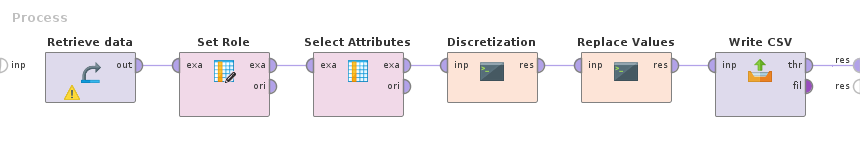
\includegraphics[width=1\textwidth]{images/rapidminer-process}
		\caption{Hauptprocess}
		\label{fig:recherche:rapidminer:1:1}
	\end{subfigure} \\
	\begin{subfigure}[t]{0.5\textwidth}
		\centering
		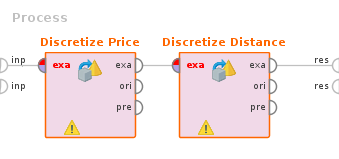
\includegraphics[width=1\textwidth]{images/rapidminer-process-discretization}
		\caption{Subprocess für die Diskretisierung}
		\label{fig:recherche:rapidminer:1:2}
	\end{subfigure}
	\begin{subfigure}[t]{0.8\textwidth}
		\centering
		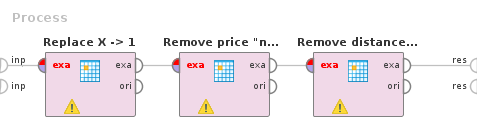
\includegraphics[width=1\textwidth]{images/rapidminer-process-replace-values}
		\caption{Subprocess für die Ersetzung von Attributwerten}
		\label{fig:recherche:rapidminer:1:3}
	\end{subfigure}
	\caption{RapidMiner Prozess für die Vorbereitung der Daten}
	\label{fig:recherche:rapidminer:1}
\end{figure}

\chapter{Testing \& Fazit}
\label{sec:testingfazit}

\section{Mögliche Erweiterungen/Verbesserungen}
Diskretiesierungsschritte \cref{sec:recherche:datenvorbereitung} nach Häufigkeitsanalyse.
Z.b. die Preise plotten -> man sieht ein peek bei CHF1000/Buchung. +/- 1/3 vom Peek sind die normalen Preise. Darunter Budget, darüber Luxury

\gls{optics} einsetzen um $\epsilon$ bei \gls{dbscan} zu eliminieren.

Hierarchical clustering einsetzen. Allerdings weniger performant und deshalb schlecht fürs explorieren geeignet.

\appendix
\chapter{Feldbeschreibungen}
\label{app:feldbeschreibungen}
Nachfolgend werden die Felder der Daten beschrieben.

Es gibt dabei folgende Datentypen:
\begin{itemize}
\item integer: geordnete Ganzzahlen $\mathbb{Z}$
\item date: Datum im Format yyyy-mm-dd (y = year, m = month, d = day)
\item categorical: Limitierte Liste von ungeordneten Werten
\item boolean: Attribut kann zwei Werte, "`wahr"' oder "`falsch"', annehmen. 
\item string: Beliebiger ungeordneter Text.
\item float: geordnete reelle Zahl $\mathbb{R}$
\end{itemize}

\rowcolors{1}{tablebodycolor}{tablerowcolor}
\begin{longtable}{ | c | c | c | L{7.5cm} | } 
	\hline 
	\rowcolor{tableheadcolor}
	\bfseries Zelle & \bfseries Name & \bfseries Datentyp & \bfseries Beschreibung \\ \hline 
	
	\rowcolor{tableheadcolor}
	\multicolumn{4}{|c|}{\textbf{Buchungsdaten}} \\ \hline
	A & RESNRDIS & integer & Eindeutige Buchungsnummer \\ \hline 
	B & RESINSDATE & date & Erstellungsdatum der Buchung \\ \hline 
	C & BOOKSTA & categorical & Status der Buchung \\ \hline 
	D & SELCURR & categorical & Währung \\ \hline 
	E & PRICES & integer & Preis \\ \hline 
	F & SONR & categorical & Sales Office Nummer \\ \hline 
	G & MAINSONR & categorical & Main Sales Office Nummer \\ \hline 
	H & BOOKLANG & categorical & Sprache der Benutzers \\ \hline 
	I & NREF & categorical & Nummer des gebuchten Objekts \\ \hline 
	J & RESBEGDATE & date & Startdatum des Aufenthaltes \\ \hline 
	K & RESENDDATE & date & Enddatum des Aufenthaltes \\ \hline 
	L & REPAX & integer & Anzahl Passagiere \\ \hline 
	M & READULT & integer & Anzahl Erwachsene \\ \hline 
	N & RECHILD & integer & Anzahl Kinder \\ \hline 
	O & REBABY & integer & Anzahl Babies \\ \hline 
	P & CUTITLE & categorical & Anrede des Kunden \\ \hline 
	Q & CUNAME & string & Name des Kunden \\ \hline 
	R & CUSTRAS & string & Strasse des Kunden \\ \hline 
	S & CUCNTRY & categorical & Land des Kunden \\ \hline 
	T & CUZIP & integer & Postleitzahl des Kunden \\ \hline 
	U & CUORT & string & Ortschaft des Kunden \\ \hline 
	
	\rowcolor{tableheadcolor}
	\multicolumn{4}{|c|}{\textbf{Objektdaten}} \\ \hline
	V & OBGEOLAT & float & Breitengrad des Objekts \\ \hline 
	W & OBGEOLONG & float & Längengrad des Objekts \\ \hline 
	X & OBSTRAS & string & Strasse des Objekts \\ \hline 
	Y & OBCNTRY & categorical & Land des Objekts \\ \hline 
	Z & OBZIP & integer & Postleitzahl des Objekts \\ \hline 
	AA & OBORT & string & Ortschaft des Objekts \\ \hline 
	AB & PAX & string & Anzahl möglicher Gäste \\ \hline 
	AC & QUAL & string & Sterne Bewertung des Objekts \\ \hline 
	AD & ROOMS & string & Anzahl Zimmer \\ \hline 
	AE & BEDROOMS & string & Anzahl Schlafzimmer \\ \hline 
	AF & BRAND & categorical & Provider des Objekts. A = Villa Vacant, B = Bungalow.Net, C = Interchalet, DAC = Dan Center, D = Sol og Strang, E = DanCenter, F = Belvilla, FER = Feratel, G = Adagio, H = Hotelpac, I = Interhome, J = Just France, JAS = Jassu Travel, L = Lomarengas, M = HR Special Residence, NFM = Norddeich Ferienwohnungen Maus GmbH, O = Roompot, P = Topic Travel, Q = Aquadelta, R = Resortquest, S = TOMAS, T = Tui Wolters, V = Vacando, W = PO for IH, Y = Centerparcs, Z = Sunpars, IL = Interhome Light, TAB = Total Accommodation Booking System, APA = Apartments Apart, PVI = Portvil, AMA = Interhome, SPR = Swisspeak Resorts\\ \hline 
	AG & ACCOMTYPE & categorical & Typ des Objekts\\ \hline 
	AH & PETS & boolean & Haustiere erlaubt? \\ \hline 
	AI & CHOUSE & categorical & A = Apartment (Wohnung), H = ) \\ \hline 
	AJ & HOUSETYPE & categorical & Typ des Hauses ??? \\ \hline 
	AK & DIWATER & integer & Distanz zum Wasser (m) \\ \hline 
	AL & DISKI & integer & Distanz zum Skigebiet (m) \\ \hline 
	AM & DIPUBT & integer & Distanz zum öffentlichen Verkehr (m) \\ \hline 
	AN & DIGOLF & integer & Distanz zum Golfplatz (m) \\ \hline 
	AO & CNATURE & boolean & Naturbelassene Umgebung \\ \hline 
	AP & CTRANQUILI & boolean & Ruhige Umgebung \\ \hline 
	AQ & CBATHANDSH & boolean & Bad oder eine Dusche im Objekt \\ \hline 
	AR & CAIRCOND & boolean & Aircondition im Objekt\\ \hline 
	AS & CCENTRAL & boolean & Objekt liegt zentral gelegen \\ \hline 
	AT & CSUNNY & boolean & Umgebung des Objekts ist sonnig \\ \hline 
	AU & CFENCED & boolean & Objekt ist umzäunt \\ \hline 
	AV & CGARDEN & boolean & Objekt besitzt einen Garten \\ \hline 
	AW & CPOOL & boolean & Objekt besitzt einen Pool \\ \hline 
	AX & CPPOOL & boolean & Objekt besitzt einen privaten Pool \\ \hline 
	AY & CHEATED & boolean & Objekt besitzt einen geheizten Pool \\ \hline 
	AZ & CSAFEPOOL & boolean & Objekt besitzt einen sicheren Pool \\ \hline 
	BA & CCHILDPOOL & boolean & Objekt besitzt einen kindersicheren Pool \\ \hline 
	BB & CTENNIS & boolean & Objekt besitzt einen Tennisplatz \\ \hline 
	BC & CBBQ & boolean & Objekt besitzt einen Grill \\ \hline 
	BD & CRECEPTION & boolean & Objekt besitzt eine Rezeption \\ \hline 
	BE & CRESTAURAN & boolean & Objekt besitzt ein Restaurant \\ \hline 
	BF & CSAUNA & boolean & Objekt besitzt eine Saune \\ \hline 
	BG & CFITNESS & boolean & Objekt besitzt ein Fitness \\ \hline 
	BH & CMASSAGE & boolean & Massagen können bezogen werden \\ \hline 
	BI & CJACUZZI & boolean & Objekt besitzt ein Jacuzzi \\ \hline 
	BJ & CBILLARD & boolean & Objekt besitzt einen Billiardtisch \\ \hline 
	BK & CTABLETENN & boolean & Objekt besitzt einen Tischtennis Tisch \\ \hline 
	BL & CELEVATOR & boolean & Objekt besitzt einen Lift \\ \hline 
	BM & CWASHMACHI & boolean & Objekt besitzt eine Waschmaschine \\ \hline 
	BN & CDRYER & boolean & Objekt besitzt einen Trockner \\ \hline 
	BO & CCHANGELIN & boolean & Es gibt einen Service um die Bettwäsche zu wechseln \\ \hline 
	BP & CCLEANING & boolean & Es gibt einen Reinigungsservice \\ \hline 
	BQ & CMAIDENSER & boolean & Es gibt einen Aufräumservice \\ \hline 
	BR & CFRESHBREA & boolean & Frisches Brot kann in nächster Umgebung bezogen werden \\ \hline 
	BS & CBREAKFAST & boolean & Es kann in nächster Umgebung gefrühstückt werden \\ \hline 
	BT & CHALFBOARD & boolean & Es wird halbpension angeboten \\ \hline 
	BU & CPARKING & boolean & Es gibt einen Parkplatz \\ \hline 
	BV & CDISHWASHE & boolean & Objekt besitzt einen Geschirrspühler \\ \hline 
	BW & CFIREPLACE & boolean & Objekt besitzt ein Cheminée \\ \hline 
	BX & SCTV & boolean & Objekt besitzt einen Fernseher \\ \hline 
	BY & SCBALCONY & boolean & Objekt besitzt ein Balkon \\ \hline 
	BZ & SCFREEZER & boolean & Objekt besitzt einen Tiefkühler \\ \hline 
	CA & SCNOSMOKE & boolean & Im Objekt darf nicht geraucht werden \\ \hline 
	CB & CSNATURECO & boolean & Naturbelassene Umgebung im Sommer \\ \hline 
	CC & CWNATURECO & boolean & Naturbelassene Umgebung im Winter \\ \hline 
	CD & CBATHSEA & boolean & In der Umgebung kann im Mehr gebadet werden \\ \hline 
	CE & CBATHLAKE & boolean & In der Umgebung kann in einem See gebadet werden \\ \hline 
	CF & CMOUNTLAKE & boolean & In der Umgebung kann in einem Bergsee gebadet werden \\ \hline 
	CG & CSRESTRELA & boolean & ??? \\ \hline 
	CH & CWRESTRELA & boolean & ??? \\ \hline 
	CI & CMETROPOLI & boolean & Objekt liegt in einer Metropole \\ \hline 
	CJ & CHIKINGMOU & boolean & In der Umgebung kann kann in den Bergen gewandert werden \\ \hline 
	CK & CHIKINGPLA & boolean & In der Umgebung kann  \\ \hline 
	CL & CNORDICWAL & boolean & In der Umgebung kann im Flachland gewandert werden \\ \hline 
	CM & CSACTFUNSP & boolean & In der Umgebung kann im Sommer Aktivsport betrieben werden \\ \hline 
	CN & CWACTFUNSP & boolean & In der Umgebung kann im Winter Aktivsport betrieben werden \\ \hline 
	CO & CENTERPARK & boolean & In der Umgebung kann gibt es ein Vergnügungspark \\ \hline 
	CP & CBIKINGMOU & boolean & In der Umgebung kann in den Bergen Fahrrad gefahren werden \\ \hline 
	CQ & CBIKINGPLA & boolean & In der Umgebung kann im Flachland Fahrrad gefahren werden \\ \hline 
	CR & CSAILING & boolean & In der Umgebung kann kann gesegelt werden \\ \hline 
	CS & CSURFING & boolean & In der Umgebung kann man surfen \\ \hline 
	CT & CWINDSURF & boolean & In der Umgebung kann windsurfen \\ \hline 
	CU & CSNIGHTLIF & boolean & In der Umgebung gibt es Nachtleben im Sommer \\ \hline 
	CV & CWNIGHTLIF & boolean & In der Umgebung gibt es Nachtlegen im Winter \\ \hline 
	CW & CSSENIOR & boolean & Objekt ist im Sommer seniorentauglich \\ \hline 
	CX & CWSENIOR & boolean & Objekt ist im Winter seniorentauglich \\ \hline 
	CY & CSFAMILY & boolean & Objekt ist im Sommer familientauglich \\ \hline 
	CZ & CWFAMILY & boolean & Objekt ist im Winter familientauglich \\ \hline 
	DA & CSIDYLIC & boolean & Objekt ist im Sommer idyllisch \\ \hline 
	DB & CWIDYLIC & boolean & Objekt ist im Winter idyllisch \\ \hline 
	DC & CHISTORIC & boolean & Objekt liegt in einer historischen Umgebung \\ \hline 
	DD & CWINEDINE & boolean & ??? \\ \hline 
	DE & CSUITHOMO & boolean & ??? \\ \hline 
	DF & CTYPVILLAG & boolean & Objekt liegt in einem Dorf \\ \hline 
	DG & CCOVERPARK & boolean & ??? \\ \hline 
	DH & CTYPRUSTIC & boolean & Objekt ist rustikal eingerichtet \\ \hline 
	DI & CTYPCOMFOR & boolean & Objekt ist konfortabel eingerichtet \\ \hline 
	DJ & CTYPLUXUR & boolean & Objekt ist luxuriös eingerichtet \\ \hline 
	DK & CTYPMODERN & boolean & Objekt ist modern eingerichtet \\ \hline 
	DL & CTYPHISTOR & boolean & Objekt ist historisch eingerichtet \\ \hline 
	DM & AIRPORT1 & categorical & IATA Code des nächsten Flughafen \\ \hline 
	DN & DIAIRPORT1 & integer & Distanz bis zum nächsten Flughafen (km) \\ \hline 
	DO & CROSSSKIIN & boolean & In der Umgebung kann Crossski gefahren werden \\ \hline 
	DP & ICERINK & boolean & In der Umgebung gibt es eine Eisbahn \\ \hline 
	DQ & SKIAREA & boolean & In der Umgebung gibt es ein Skigebiet \\ \hline 
	DR & SNOWBOARD & boolean & In der Umgebung kann Snowboard gefahren werden \\ \hline 
	DS & TOBOGGAN & boolean & In der Umgebung kann man Rodeln \\ \hline 
	DT & WINTERWALK & boolean & In der Umgebung kann man im Winter wandern \\ \hline 
	DU & OUTDPOOL & categorical & Objekt besitzt einen aussen Pool \\ \hline 
	DV & INDPOOL & boolean & Objekt besitzt einen innen Pool \\ \hline 
	DW & DVDPLAYER & boolean & Objekt besitzt einen DVD Player \\ \hline 
	DX & PTENNIS & boolean & Objekt besitzt einen privaten Tennisplatz \\ \hline 
	DY & SOLARIUM & boolean & Objekt besitzt ein Solarium \\ \hline 
	DZ & DICENTER & integer & Distanz bis zum Zentrum (m) \\ \hline 
	EA & DISEA & integer & Distanz bis zum Meer (m) \\ \hline 
	EB & DILAKE & integer & Distanz bis zum See (m) \\ \hline 
	EC & CRESIDENCE & boolean & Objekt ist eine Residenz \\ \hline 
	ED & CPTENNIS & boolean & Objekt besitzt einen privaten Tennisplatz \\ \hline 
	EE & CHORSE & boolean & In der Umgebung kann man reiten \\ \hline 
	EF & CVIEWSEA & boolean & Objekt besitzt eine Aussicht auf das Meer \\ \hline 
	EG & INTERNET & boolean & Objekt besitzt Internet \\ \hline 
	EH & CHILDPGRND & boolean & Objekt besitzt einen Kinderspielplatz \\ \hline 
	EI & CISLAND & boolean & Objekt liegt auf einer Insel \\ \hline 
	EJ & CVIEWMOUNT & boolean & Objekt besitzt eine Aussicht auf die Berge \\ \hline 
	EK & CVIEWCNTRY & boolean & Objekt besitzt eine Aussicht auf das Flachland \\ \hline 
	EL & CVIEWLAKE & boolean & Objekt besitzt eine Aussicht auf einen See \\ \hline 
	EM & CBATH & boolean & Objekt besitzt ein Bad \\ \hline 
	EN & CSHOWER & boolean & Objekt besitzt eine Dusche \\ \hline 
	EO & CCARPORT & boolean & ??? \\ \hline 
	EP & CSGARAGE & boolean & ??? \\ \hline 
	EQ & CCGARAGE & boolean & ??? \\ \hline 
	ER & CGOLFCOURS & boolean & In der Umgebung gibt es einen Golfplatz \\ \hline 
	ES & CWELLNESS & boolean & In der Umgebung gibt es ein Wellness \\ \hline 
	ET & CMICROWAVE & boolean & Objekt besitzt eine Mikrowelle \\ \hline 
	EU & COVEN & boolean & Objekt besitzt einen Ofen \\ \hline 
	EV & CPHONE & boolean & Objekt besitzt ein Telefon \\ \hline 
	EW & CTERRACE & boolean & Objekt besitzt eine Terasse \\ \hline 
	\caption{Attributbeschreibung}
\end{longtable} 

\chapter{Testdatenquellen}
\label{app:testdatenquellen}

%\num[round-mode=places,round-precision=7]{}
\csvstyle{myTableStyle}{tabular=|c|c||c|c|c|c|c|c||c|c|,
	separator=semicolon,
	table head=\hline \rowcolor{tableheadcolor} \multicolumn{2}{|c||}{General} & \multicolumn{6}{c||}{Categorical} & \multicolumn{2}{c|}{Numerical} \\\hline
	\rowcolor{tableheadcolor} \rotatebox{90}{id} & \rotatebox{90}{NREF} & \rotatebox{90}{Distanz zum Wasser} & \rotatebox{90}{Distanz zum ÖV} & \rotatebox{90}{Distanz zum Meer} & \rotatebox{90}{Wochenpreis} & \rotatebox{90}{Haustiere erlaubt} & \rotatebox{90}{Aircondition vorhanden} & \rotatebox{90}{Anzahl Zimmer} & \rotatebox{90}{Anzahl Schlafzimmer} \\ ,
	late after line=\\,
	late after last line=\\\hline,
	head to column names}


\section{TC1: 2 gleiche Distanzattribute}
\label{app:testdatenquellen:1}

\csvreader[myTableStyle]%
{testcases/data-apriori-2-entries--2-distances.csv}
{}
{\id & \NREF & \DIWATER & \DIPUBT & \DISEA & \weeklyprice & \PETS & \CAIRCOND & \ROOMS & \BEDROOMS}

\section{TC2: 2 gleiche Binärattribute}
\label{app:testdatenquellen:2}

\csvreader[myTableStyle]%
{testcases/data-apriori-2-entries--2-binary-attributes.csv}
{}
{\id & \NREF & \DIWATER & \DIPUBT & \DISEA & \weeklyprice & \PETS & \CAIRCOND & \ROOMS & \BEDROOMS}

\section{TC3: 2 gleiche numerische Attribute}
\label{app:testdatenquellen:3}

\csvreader[myTableStyle]%
{testcases/data-apriori-2-entries--2-numeric-attributes.csv}
{}
{\id & \NREF & \DIWATER & \DIPUBT & \DISEA & \weeklyprice & \PETS & \CAIRCOND & \ROOMS & \BEDROOMS}

\section{TC4: 1 numerisches und 1 Binärattribut}
\label{app:testdatenquellen:4}

\csvreader[myTableStyle]%
{testcases/data-apriori-2-entries--1-numeric-1-binary-attribute.csv}
{}
{\id & \NREF & \DIWATER & \DIPUBT & \DISEA & \weeklyprice & \PETS & \CAIRCOND & \ROOMS & \BEDROOMS}

\section{TC5: 2 gleiche Distanzattribute mit einem Binärfilter}
\label{app:testdatenquellen:5}

\csvreader[myTableStyle]%
{testcases/data-apriori-2-entries--binary-filter--2-distances.csv}
{}
{\id & \NREF & \DIWATER & \DIPUBT & \DISEA & \weeklyprice & \PETS & \CAIRCOND & \ROOMS & \BEDROOMS}

\section{TC6: 2 gleiche Distanzattribute mit einem Distanzfilter}
\label{app:testdatenquellen:6}

\csvreader[myTableStyle]%
{testcases/data-apriori-2-entries--distance-filter--2-distances.csv}
{}
{\id & \NREF & \DIWATER & \DIPUBT & \DISEA & \weeklyprice & \PETS & \CAIRCOND & \ROOMS & \BEDROOMS}

\section{TC7: 2 gleiche Distanzattribute mit einem numerischen Filter}
\label{app:testdatenquellen:7}

\csvreader[myTableStyle]%
{testcases/data-apriori-2-entries--number-filter--2-distances.csv}
{}
{\id & \NREF & \DIWATER & \DIPUBT & \DISEA & \weeklyprice & \PETS & \CAIRCOND & \ROOMS & \BEDROOMS}

\section{TC8: 2 gleiche Distanz- und 1 binäres Attribut}
\label{app:testdatenquellen:8}

\csvreader[myTableStyle]%
{testcases/data-apriori-3-entries--2-distances-1-binary.csv}
{}
{\id & \NREF & \DIWATER & \DIPUBT & \DISEA & \weeklyprice & \PETS & \CAIRCOND & \ROOMS & \BEDROOMS}

\section{TC9: Zwei Menten mit einmal 2 Distanzen und einmal 1 numerischen und 1 Binärattritbut}
\label{app:testdatenquellen:9}

\csvreader[myTableStyle]%
{testcases/data-apriori-3-entries-two-sets--2-distances--1-number-1-binary.csv}
{}
{\id & \NREF & \DIWATER & \DIPUBT & \DISEA & \weeklyprice & \PETS & \CAIRCOND & \ROOMS & \BEDROOMS}

\section{TC10: 2 Clusters mit jeweils 5 Elementen}
\label{app:testdatenquellen:10}

\csvreader[myTableStyle]%
{testcases/data-cluster-2-entries--2-clusters--5-and-5--0-distance.csv}
{}
{\id & \NREF & \DIWATER & \DIPUBT & \DISEA & \weeklyprice & \PETS & \CAIRCOND & \ROOMS & \BEDROOMS}

\section{TC11: 1 Cluster mit 1 Element und 1 Cluster mit 9 Elementen}
\label{app:testdatenquellen:11}

\csvreader[myTableStyle]%
{testcases/data-cluster-2-entries--2-clusters--9-and-1--0-distance.csv}
{}
{\id & \NREF & \DIWATER & \DIPUBT & \DISEA & \weeklyprice & \PETS & \CAIRCOND & \ROOMS & \BEDROOMS}

\section{TC12: 2 Cluster mit kleinen Unterschieden}
\label{app:testdatenquellen:12}

\csvreader[myTableStyle]%
{testcases/data-cluster-minor-differences-2-entries--2-clusters--5-and-5--0-distance.csv}
{}
{\id & \NREF & \DIWATER & \DIPUBT & \DISEA & \weeklyprice & \PETS & \CAIRCOND & \ROOMS & \BEDROOMS}



\chapter{Klassendiagramme}
\label{app:klassendiagram}
Nachfolgend werden die Klassendiagramme präsentiert. Die Erklärung dazu ist im \cref{sec:proofofconcept:klassenstruktur} zu finden.
\begin{figure}[H]
	\centering
	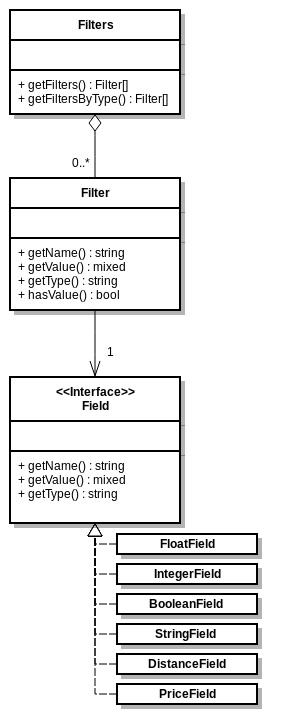
\includegraphics[width=0.5\textwidth]{images/diagram-class-filters}
	\caption{Klassendiagramm der Filter und Felder Datenmodelle}
	\label{fig:proofofconcept:klassenstruktur:5}
\end{figure}
\begin{figure}[H]
	\centering
	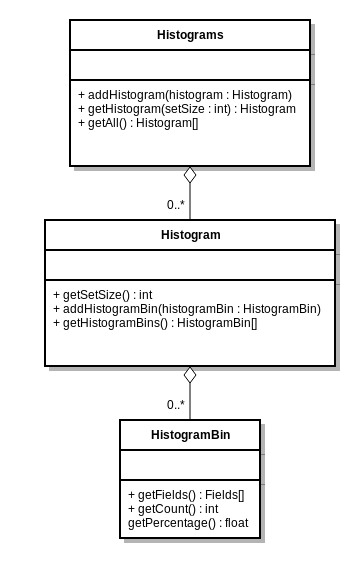
\includegraphics[width=0.6\textwidth]{images/diagram-class-Histograms}
	\caption{Klassendiagramm der Histogram-Modelle}
	\label{fig:proofofconcept:klassenstruktur:6}
\end{figure}
\begin{sidewaysfigure}[H]
	\centering
	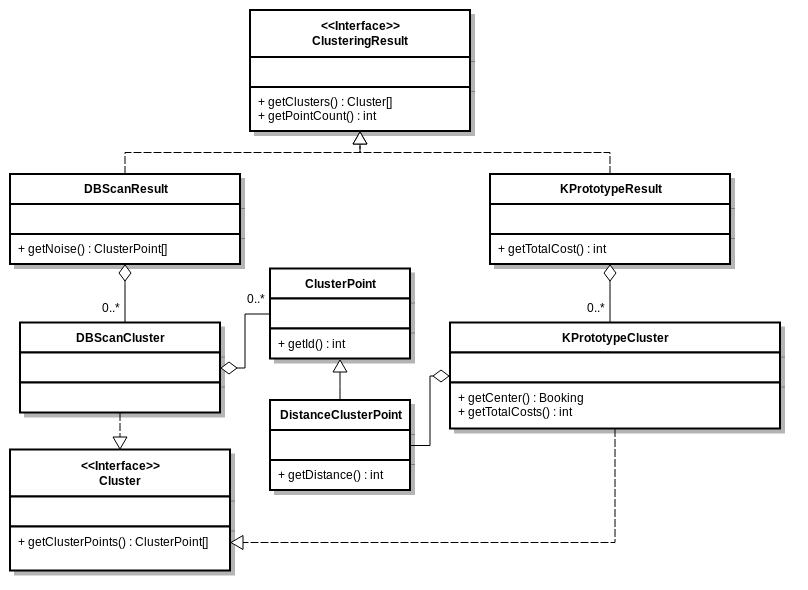
\includegraphics[width=1\textwidth]{images/diagram-class-clusters}
	\caption{Klassendiagramm der Clusterresultate}
	\label{fig:proofofconcept:klassenstruktur:7}
\end{sidewaysfigure}
\begin{figure}[H]
	\centering
	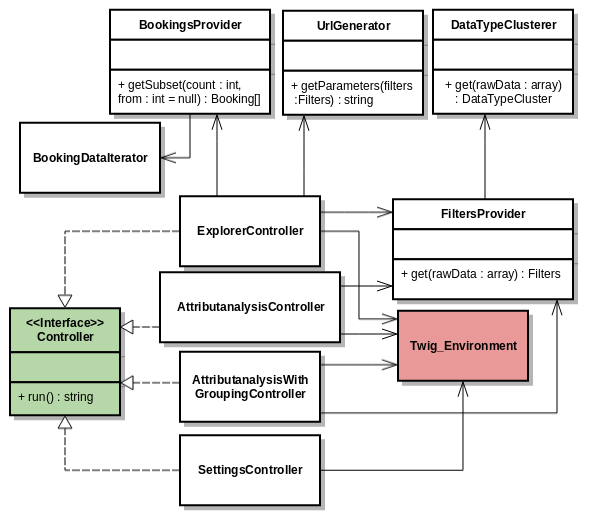
\includegraphics[width=1\textwidth]{images/diagram-class-Controller}
	\caption{Klassendiagramm der Controller}
	\label{fig:proofofconcept:klassenstruktur:1}
\end{figure}
\begin{sidewaysfigure}[H]
	\centering
	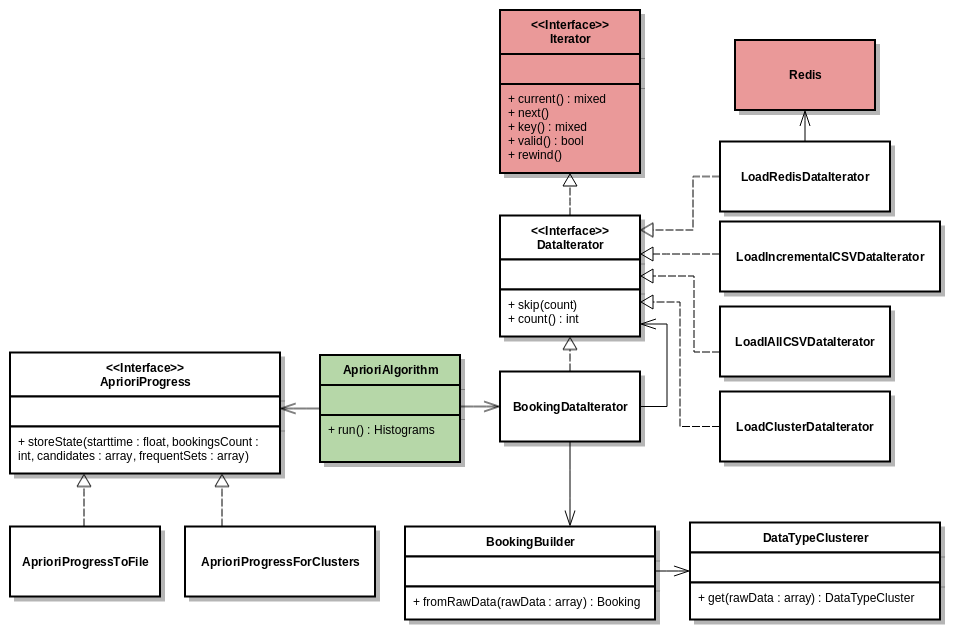
\includegraphics[width=1\textwidth]{images/diagram-class-AprioriAlgorithm}
	\caption{Klassendiagramm des Apriori Alogorithmus}
	\label{fig:proofofconcept:klassenstruktur:2}
\end{sidewaysfigure}
\begin{figure}[H]
	\centering
	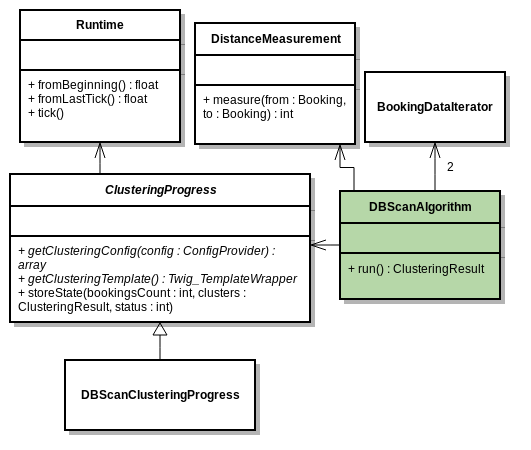
\includegraphics[width=1\textwidth]{images/diagram-class-DBScanAlgorithm}
	\caption{Klassendiagramm des DBScan Alogorithmus}
	\label{fig:proofofconcept:klassenstruktur:3}
\end{figure}
\begin{figure}[H]
	\centering
	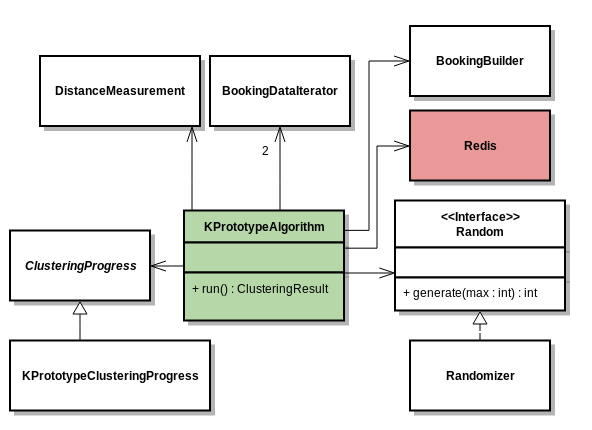
\includegraphics[width=1\textwidth]{images/diagram-class-KPrototypeAlgorithm}
	\caption{Klassendiagramm des KPrototype Alogorithmus}
	\label{fig:proofofconcept:klassenstruktur:4}
\end{figure}

\chapter{Ansichten des Programms}
Nachfolgend werden Ansichten des Programms aufgezeigt, die in der Proof of Concept Phase umgesetzt wurden.
\label{app:pocansichten}
\begin{figure}[H]
	\RawFloats
	\centering
	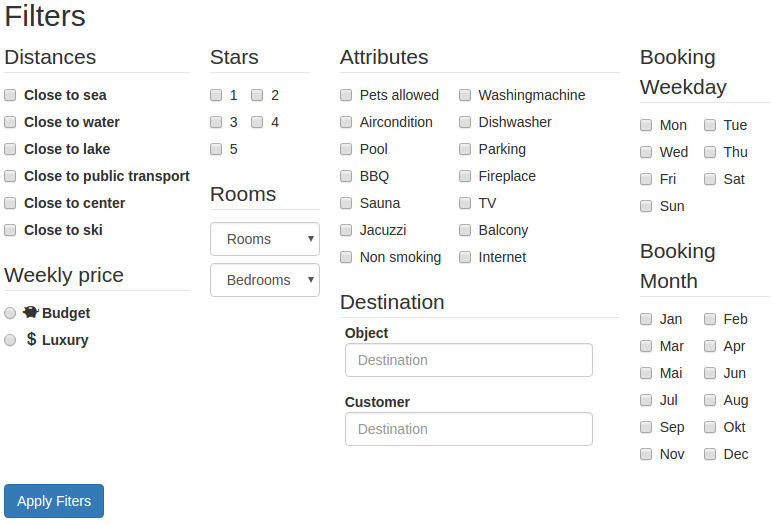
\includegraphics[width=1\textwidth]{images/program-filters}
	\caption{Ansichten des Programms: Filters}
\end{figure}
\begin{figure}[H]
	\RawFloats
	\centering
	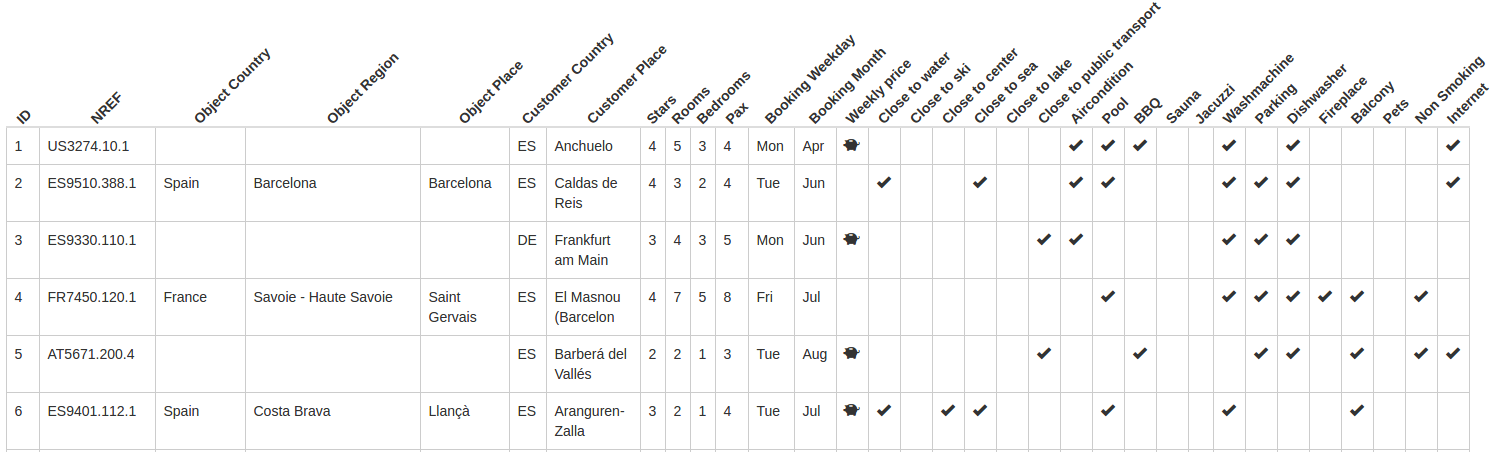
\includegraphics[width=1\textwidth]{images/program-explore-results}
	\caption{Ansichten des Programms: Stammdaten einsehen}
\end{figure}
\begin{figure}[H]
	\RawFloats
	\centering
	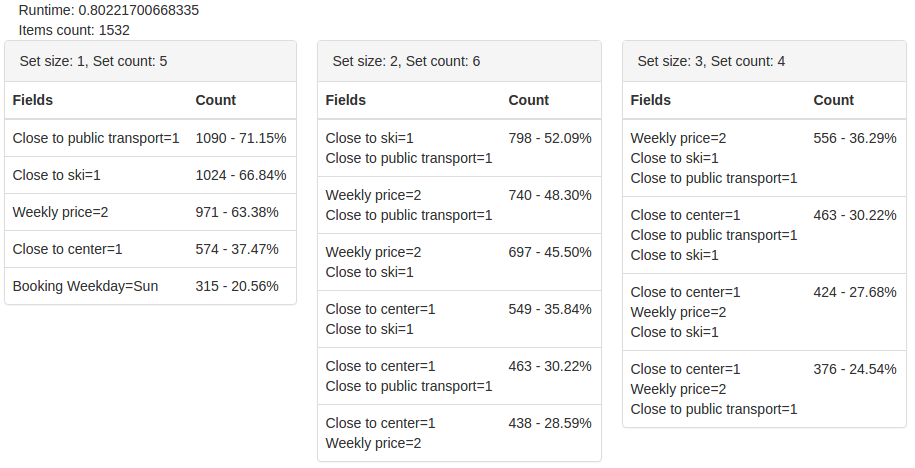
\includegraphics[width=1\textwidth]{images/program-apriori-results}
	\caption{Ansichten des Programms: Resultat einer Apriori Analyse}
\end{figure}
\begin{figure}[H]
	\RawFloats
	\centering
	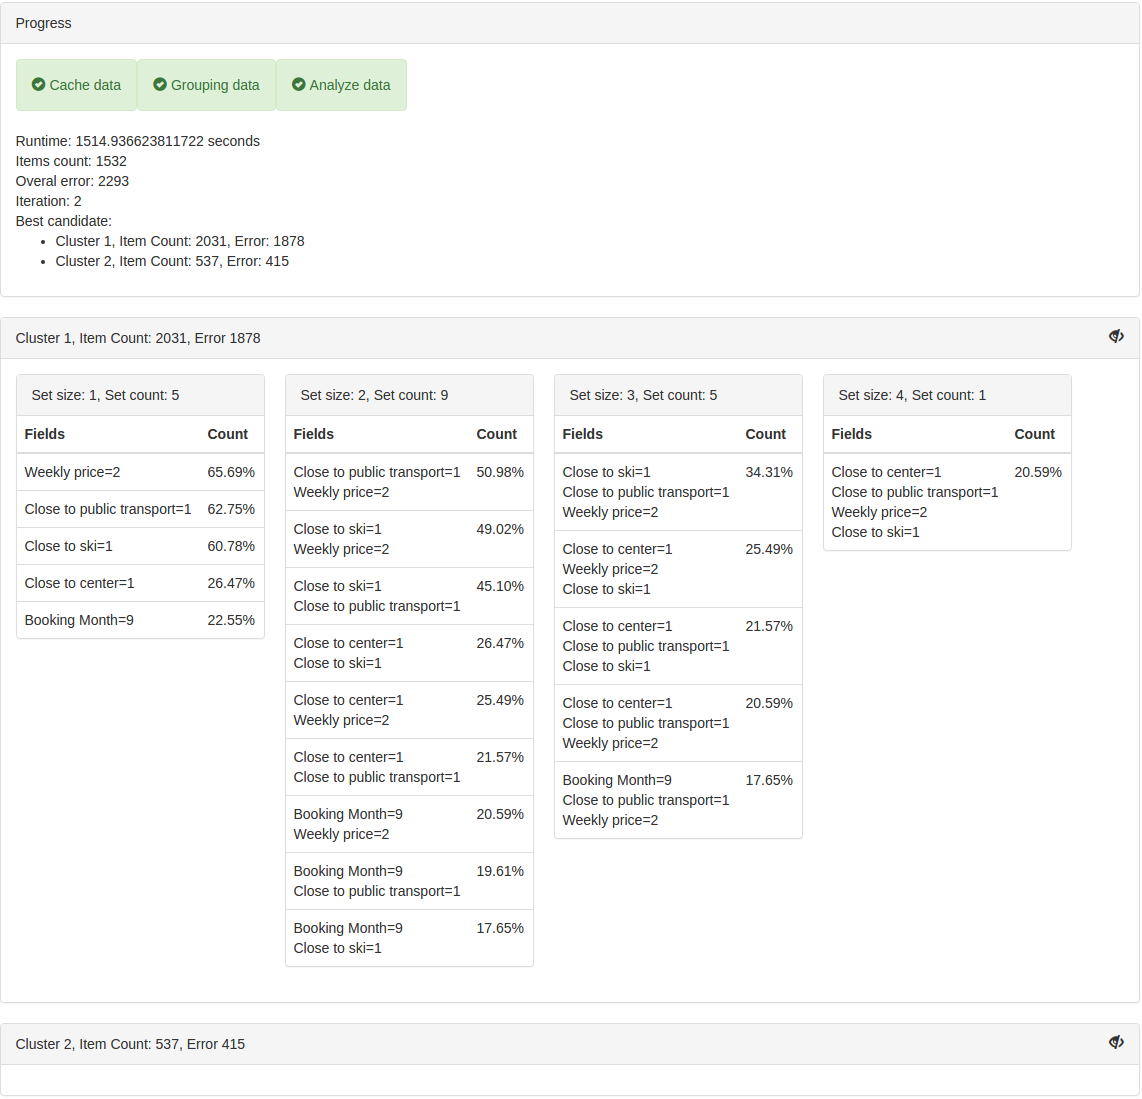
\includegraphics[width=1\textwidth]{images/program-kprototype-results}
	\caption{Ansichten des Programms: Resultat einer k-prototype Analyse}
\end{figure}
\begin{figure}[H]
	\RawFloats
	\centering
	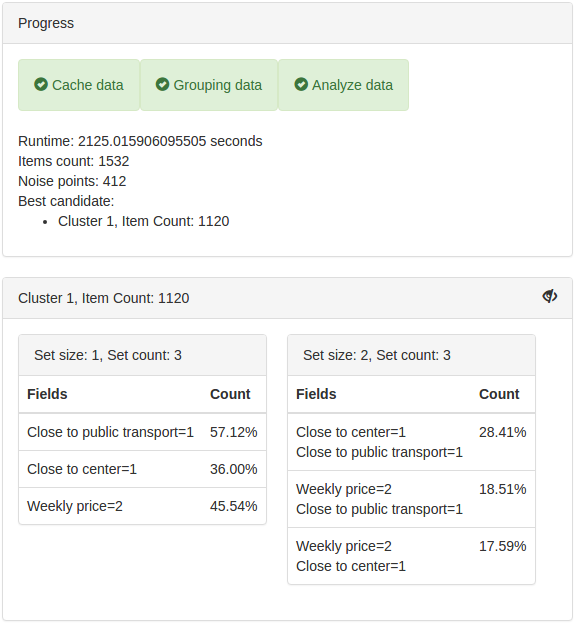
\includegraphics[width=0.8\textwidth]{images/program-dbscan-results}
	\caption{Ansichten des Programms: Resultat einer DBSCAN Analyse}
\end{figure}
\begin{figure}[H]
	\RawFloats
	\centering
	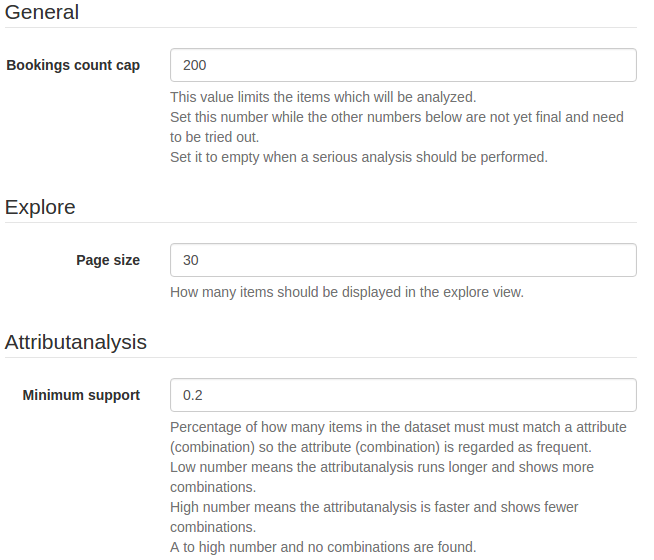
\includegraphics[width=1\textwidth]{images/program-settings}
	\caption{Ansichten des \textbf{Programms}: Ausschnitt der Ansicht "`Algorithmen konfigurieren"'}
\end{figure}



% % !TeX encoding=utf8
% !TeX spellcheck = en-US

\chapter{Experiments}

% remove this line once you start adding your real content.
% !TeX encoding=utf8
% !TeX program = pdflatex
% !TeX spellcheck = en-US

% LaTeX Tutorial for the latexthesistemplate
% based on 
% - https://pangea.stanford.edu/computing/unix/formatting/latexexample.php
% - http://sip.clarku.edu/tutorials/TeX/
% and extended and modified by Matthias Pospiech

\ifcsdef{cs}{}{\newcommand{\cs}[1]{\texttt{\textbackslash{}#1}\relax}}%

% Define colors in case they are not available because style.tex was 
% not loaded
% table colors 
\colorlet{tablebodycolor}{white!100}
\colorlet{tablerowcolor}{gray!10}
\colorlet{tablesubheadcolor}{gray!30}
\colorlet{tableheadcolor}{gray!25}

\section{LaTeX Typesetting By Example}
\label{sec:example:tutorial}
This section demonstrates a basic set of LaTeX formatting commands and shows how they look like in this template. For comparison of the typeset output with the input document refer to the code listing starting on page \pageref{sec:example:code}.

The content presented here is based on similar text by Phil Farrell\footnote{\url{https://pangea.stanford.edu/computing/unix/formatting/latexexample.php}} and Harvey Gould\footnote{\url{http://sip.clarku.edu/tutorials/TeX/}}.
For further reading on the possibilities of this template please refer to the documentation: \path{TemplateDocumentation.pdf}.

% ~~~~~~~~~~~~~~~~~~~~~~~~~~~~~~~~~~~~~~~~~~~~~~~~~~~~~~~~~~~~~~~~~~~~~~~~~
\subsection{Plain Text}
\label{sec:example:PlainText}
\index{example!text}

Type your text in free-format; lines can be as long
or as short as you wish.
        You can indent         or space out
        your input 
            text in 
                any way you like to highlight the structure
        of your manuscript and make it easier to edit.
LaTeX fills lines and adjusts spacing between words to produce an
aesthetically pleasing result.

Completely blank lines in the input file break your text into
paragraphs.
Several command exist to change the font for a single character, word, or set of words. Simply enclose the word and within braces of the formating command, 
\emph{like this}.
A font changing command not enclosed in braces, like the change to \bfseries 
bold here, keeps that change in effect until the end of the document or
until countermanded by another font switch, like this change back to 
\normalfont the default font. 

% ~~~~~~~~~~~~~~~~~~~~~~~~~~~~~~~~~~~~~~~~~~~~~~~~~~~~~~~~~~~~~~~~~~~~~~~~~
\subsection{Font shapes}
\label{sec:example:FontShapes}
\index{example!font shapes}

The default font in the template is Latin Modern (lmodern). It includes \textit{italics}, \textbf{boldface}, \textsl{slanted}, \textsc{small caps} and \texttt{monospaced} fonts as well as the corresponding sans serif variants  of the same font family \textsf{sans serif}, \textsf{\textit{italics}}, \textsf{\textbf{boldface}} and \textsf{\textsl{slanted}}. Note that for other fonts not all font shapes may be available. 

% ~~~~~~~~~~~~~~~~~~~~~~~~~~~~~~~~~~~~~~~~~~~~~~~~~~~~~~~~~~~~~~~~~~~~~~~~~
\subsection{Quotation and Citations}
\label{sec:example:QuoteCite}
\index{example!quote}
\index{example!cite}
%
LaTeX provides the \enquote{quote} and \enquote{quotation} environments for typesetting quoted material or any other text that should be slightly indented 
and set off from the normal text.

However, if the text shall not just be indented but rather be a real quotation with a citation of the origin, then the commands \enquote{enquote} for inline quotes and \enquote{blockquote} for multi line quotes are more appropriate. The first is used to highlight the commands in this section and the latter in the following text, which is a direct quotation from the documentation of the package
 \emph{csquotes}: 
%
\blockquote[(csquotes.pdf)]{This command determines the length of the text. 
If the length exceeds a certain threshold, the text will be 
typeset in display mode, i. e., as a block quotation. 
If not, \cs{blockquote} will behave like \cs{textquote}. 
Depending on the threshold type option, the threshold may be based on the number
of lines required to typeset the text or on the number of words in the text.}

The standard command for citations is \texttt{\textbackslash{}cite} which may have a prenote argument for adding a page number or something similar. To show how a citation is typeset we cite here a book about LaTeX \cite[59]{companion}. Further commands such as \cs{parencite} \parencite{companion} and \cs{textcite} \textcite{companion} allow a different typeset of the citation. The resulting bibliography is printed out on \cpageref{sec:bibliography}. Refer to the biblatex manual for further details on citation commands and modifications on the printout and the section on biblatex in the template documentation.

% ~~~~~~~~~~~~~~~~~~~~~~~~~~~~~~~~~~~~~~~~~~~~~~~~~~~~~~~~~~~~~~~~~~~~~~~~~
\subsection{References}
\label{sec:example:references}
\index{example!references}

So far, in this text chapter and section headings, paragraphs (\cref{sec:example:PlainText}), font changes (\cref{sec:example:FontShapes}) and citations (\cref{sec:example:QuoteCite}) were demonstrated ad in this section the use of references. Not that here the command \texttt{\textbackslash{}cref} was used instead of the standard \cs{ref}.

The following sections show lists, tables and math.

% ~~~~~~~~~~~~~~~~~~~~~~~~~~~~~~~~~~~~~~~~~~~~~~~~~~~~~~~~~~~~~~~~~~~~~~~~~
\subsection{Lists}
\label{sec:example:lists}
\index{example!lists}
%
LaTeX has three types of lists with the environment names \emph{itemize}, \emph{enumerate} and \emph{description}. All lists have a separation between each item, to improve the reading of item texts spanning several lines. 
This item text can contain multiple paragraphs. These paragraphs are appropriately spaced and indented according to their position in the list.

\begin{itemize}
\item 
The \enquote{itemize} sets off list items with \emph{bullets}, like this.
%
\item Of course, lists can be nested, each type up to at least four levels.
One type of list can be nested within another type.
%
  \begin{itemize}
  \item Nested lists of the same type will change style of numbering 
  or \emph{bullets} as needed.
  \end{itemize}
\end{itemize}
%
\begin{enumerate}
\item The \enquote{enumerate} environment numbers the list elements.

This is a new paragraph in the item text, which is not intended as in the 
normal text but separated from the previous paragraph.
%
\item The enumeration scheme changes with each nesting level
  \begin{enumerate}
  \item as shown in this nested enumerated list item.
  \end{enumerate}
\end{enumerate}  
%
Don't forget to close off all list environments with the 
appropriate \verb+\end{...}+ command.
Indenting \verb+\begin{...}+, \verb+\item+, and \verb+\end{...}+
commands in the input document according to their nesting level can help 
clarify the structure.

% ~~~~~~~~~~~~~~~~~~~~~~~~~~~~~~~~~~~~~~~~~~~~~~~~~~~~~~~~~~~~~~~~~~~~~~~~~
\subsection{Tables}
\label{sec:example:tables}
\index{example!tables}
%
Tables are a little more difficult. One can achieve even the most complex and fancy layout, even spanning over multiple pages, but the code to create these tables is not necessarily the best readable one.

Table \ref{tab:Computers} is a very simple table showing data lined up in columns, where each column width is automatically calculated by LaTeX.
Notice that the tabular is centered with \cs{centering} and printed in a a smaller font to achieve a clear distinction to the normal text. The title is created above the tabular with \cs{captionabove}.

\begin{table}[hb]
\centering
\small\renewcommand{\arraystretch}{1.4}  
\captionabove{Numbers of Computers in the department, By Type.}
\label{tab:Computers}
\begin{tabular}{lr}
\hline
Mac (Apple)    & 2  \\
Windows XP, 7  & 60 \\
Linux (Server) & 10 \\
\hline
\end{tabular}
\end{table}

\Cref{tab:IsingModel} on \cpageref{tab:IsingModel} demonstrate the creation of a pleasant appearing table, which helps to read the table without attracting to much attention by the use of shaded colors. The caption uses the additional short caption in square brackets \texttt{[ ]}, which is used in the list of tables, see \cpageref{sec:lot}.

\begin{table}[ht]
\centering
\small\renewcommand{\arraystretch}{1.4}  
\rowcolors{1}{tablerowcolor}{tablebodycolor}
%
\captionabove[Mean-field predictions for the critical temperature of the Ising model]{Comparison of the mean-field predictions for the critical temperature of the Ising model with exact results and the best known estimates for different spatial dimensions $d$ and lattice symmetries.}
\label{tab:IsingModel}
%
\begin{tabularx}{0.5\textwidth}{lXXX}
\hline
\rowcolor{tableheadcolor}
lattice & $d$ & $q$ & $T_\text{mf}/T_c$ \\
\hline
square  & 2 & 4 & 1.763 \\
%
triangular & 2 & 6 & 1.648 \\
%
diamond & 3 & 4 & 1.479 \\
%
simple cubic & 3 & 6 & 1.330 \\
%
bcc & 3 & 8 & 1.260 \\
%
fcc & 3 & 12 & 1.225 \\
\hline
\end{tabularx}
\end{table}

The design and creating of complex tables is shown in much greater detail in the documentation of this template.

% ~~~~~~~~~~~~~~~~~~~~~~~~~~~~~~~~~~~~~~~~~~~~~~~~~~~~~~~~~~~~~~~~~~~~~~~~~
\subsection{Mathematical Equations}
\label{sec:example:math}
\index{example!math}

Simple equations, like $x^y$ or $x_n = \sqrt{a + b}$ can be typeset right
in the text line by enclosing them in a pair of single dollar sign symbols.
Don't forget that if you want a real dollar sign in your text, like \$2000,
you have to use the \verb+\$+ command.

A more complicated equation should be typeset in \emph{displayed math} mode using \texttt{\textbackslash{[} ... \textbackslash{]}}, like this:
%
\[
z \left( 1 \ +\  \sqrt{\omega_{i+1} + \zeta -\frac{x+1}{\Theta +1} y + 1} 
\ \right)
\ \ \ =\ \ \  1
\]
%
The \texttt{equation} environment displays your equations, and automatically
numbers them consecutively within your document, like this:
%
We can give an equation a label so that we can refer to it later.
\begin{equation}
  \label{eqn:ising}
  E = -J \sum_{i=1}^N s_i s_{i+1} ,
\end{equation}
Equation~\eqref{eqn:ising} expresses the energy of a configuration
of spins in the Ising model.\footnote{It is necessary to process (typeset) a
file twice to get the counters correct.}

For more complex formulas it may be necessary to do some fine tuning by adding small amounts of horizontal spacing, 
\begin{verbatim}
 \, small space       \! negative space
\end{verbatim}
as is done in eq.~\eqref{eqn:GreenTheorem}.
\begin{equation}
  \underset{\mathcal{G}\quad}\iiint\!
  \left[u\nabla^{2}v+\left(\nabla  u,\nabla  v\right)\right]\mathrm{d}^{3}V
  =\underset{\mathcal{S}\quad}\oiint  u\,\frac{\partial v}{\partial n}
  \,\,\mathrm{d}^{2}A
  \label{eqn:GreenTheorem}
\end{equation}
We also can also align several equations
\begin{align}
  \dot{q}_i & = \frac{\partial H}{\partial p_i} \\
  \dot{p}_i & = -\frac{\partial H}{\partial q_i} 
\end{align}
number them as subequations
\begin{subequations}
\begin{align}
  \dot{q}_i & = \frac{\partial H}{\partial p_i} \\
  \dot{p}_i & = -\frac{\partial H}{\partial q_i} 
\end{align}
\end{subequations}
or with only a single number
\begin{equation}
\begin{aligned}
  \dot{q}_i & = \frac{\partial H}{\partial p_i} \\
  \dot{p}_i & = -\frac{\partial H}{\partial q_i} 
\end{aligned}
\end{equation}
Many further possibilities of displaying equations exist. 

% ~~~~~~~~~~~~~~~~~~~~~~~~~~~~~~~~~~~~~~~~~~~~~~~~~~~~~~~~~~~~~~~~~~~~~~~~~
\subsubsection{Common Greek letters}
\label{sec:example:math:greekletters}
These commands may be used only in math mode. Only the most common
letters are included here.
%
\[\alpha, \beta, \gamma, \Gamma, \delta,\Delta,
\epsilon, \zeta, \eta, \theta, \Theta, \kappa,
\lambda, \Lambda, \mu, \nu, \xi, \Xi, \pi, \Pi,
\rho, \sigma, \tau, \phi, \Phi, \chi, \psi, \Psi,
\omega, \Omega\]

% ~~~~~~~~~~~~~~~~~~~~~~~~~~~~~~~~~~~~~~~~~~~~~~~~~~~~~~~~~~~~~~~~~~~~~~~~~
\subsection{Literal text}
\label{sec:example:verbatim}
\index{example!verbatim}
%
It is desirable to print program code exactly as it is typed in a
monospaced font. Use \cs{begin\{lstlisting\}} and
\cs{end\{lstlisting\}} as in the following example:

\begin{lstlisting}
double y0 = 10; // example of declaration and assignment statement
double v0 = 0;  // initial velocity
double t = 0;   // time
double dt = 0.01; // time step
double y = y0;
\end{lstlisting}
%
Two styles are defined in this template: \texttt{lstStyleCpp} and \texttt{lstStyleLaTeX}.

A complete file can be printed with listings using the 
command \cs{lstinputlisting}, see \cref{sec:example:code} for an example.
% ~~~~~~~~~~~~~~~~~~~~~~~~~~~~~~~~~~~~~~~~~~~~~~~~~~~~~~~~~~~~~~~~~~~~~~~~~
\subsection{Figures}
\label{sec:example:figures}
\index{example!figures}
%
Figures with captions are included in the \texttt{figure} environment in order to position the graphic inside the text. The size should be given in relation to natural text size. It is recommended to use a percentage value of the \cs{textwidth}. This size should not exceed 80\,\%  of the text width.

\begin{figure}[htb]
  \centering
  \includegraphics[width=0.4\textwidth]{images/testimage.png}
  \caption[Test image for television]{Test image for television (Origin of the image: \url{http://de.wikipedia.org/wiki/Testbild}).}
  \label{fig:example:figure}
\end{figure}

All possibilities of grouping pictures side by side, on top or in matrices can be realized. Each subfigure is created in the same way as a graphic inside a figure, just enclosed by a figure environment, as shown in \cref{fig:example:subfigures}.

\begin{figure}[htb]
  \begin{subfigure}[b]{.45\linewidth}
    \centering
    \includegraphics[width=0.5\linewidth]{images/testimage.png}
    \caption{The first subfigure.}
    \label{fig:example:subfigures:a}
  \end{subfigure}%
  \begin{subfigure}[b]{.45\linewidth}
    \centering
    \includegraphics[width=0.5\linewidth]{images/testimage.png}
    \caption{The second subfigure.}
    \label{fig:example:subfigures:b}
  \end{subfigure}
  \caption{Demonstration of the \emph{subfigure} environment inside a figure environment}
  \label{fig:example:subfigures}
\end{figure}
%
For complex subfigure constructs and correct alignment of the subcaption the \texttt{floatrow} provides powerful commands. 

% ~~~~~~~~~~~~~~~~~~~~~~~~~~~~~~~~~~~~~~~~~~~~~~~~~~~~~~~~~~~~~~~~~~~~~~~~~
\subsection{Index}
\label{sec:example:index}
\index{example!index}
%
An index is easy to create with LaTeX, but should only be done if the time is available to do it right, since it requires substantial work to create an index which is really useful for the reader.

A word is added to the index with the command \cs{index\{word\}} and these indexed words can be grouped with \cs{index\{group!word\}}. Within this document some index commands are inserted below the section headers of this tutorial for the purpose of demonstrating the indexing. The resulting index is displayed on page~\pageref{sec:Index}. 
% ~~~~~~~~~~~~~~~~~~~~~~~~~~~~~~~~~~~~~~~~~~~~~~~~~~~~~~~~~~~~~~~~~~~~~~~~~
\clearpage
\subsection{Code}
\label{sec:example:code}

\ifcsdef{lstStyleLaTeX}{%
  \lstinputlisting[style=lstStyleLaTeX,%nolol=true,%
     caption={LaTeX Typesetting By Example}, label=lstLaTeXExample]  
  {content/template/latextutorial.tex}
}{}  



%%% -- end of main content

% show all biblatex entries
\nocite{*}

% set title
\renewcommand\bibname{Quellenverzeichnis}

% -- bibliography --
% (must be placed _before_ appendix)
\IfPackageLoaded{biblatex}{
  \cleardoublepage
  \IfDefined{phantomsection}{\phantomsection}\label{sec:bibliography}
  \printbibliography[%
    heading=bibintoc, % (bibintoc, bibnumbered)
  ]
}% end of bibliography


%% -- List of Listings --
% _Remove_ if no listing with caption is defined
% \IfDefined{lstlistoflistings}{\cleardoublepage\lstlistoflistings}

% --- Appendix --- --- --- --- --- --- ---
% \cleardoublepage
% \appendix
% Add `Appendix` to TOC
% \addcontentsline{toc}{part}{\appendixname}
% must be _input_, otherwise the TOC entry is at the wrong place
% \input{content/Z-Appendix.tex}

% -- only in phd thesis --->
% \input{content/Z-Publications.tex}
% \input{content/Z-CV.tex}
% <------------------------

%% -- Index --
% _Remove_ Index unless you really want to invest a large amount
% of time and effort to create a good index!
\IfDefined{printindex}{%
  \cleardoublepage\IfDefined{phantomsection}{\phantomsection}\label{sec:index}%
  \printindex%
}% end of index

% add todo list (remove for final document!)
% \input{content/Z-Todo.tex}

%%% document END %%%%%%%%%%%%%%%%%%%%%%%%%%%%%%%%%%%%%%%%%%%%%%%%%%%%%%%%%%%
\end{document}
%%%%%%%%%%%%%%%%%%%%%%%%%%%%%%%%%%%%%%%%%%%%%%%%%%%%%%%%%%%%%%%%%%%%%%%%%%%%
